\documentclass[12pt, %
openright, 
oneside, %
%twoside, %TCC: Se seu texto tem mais de 100 páginas, descomente esta linha e comente a anterior
a4paper,    %
%english,   %
brazil]{facom-ufu-abntex2}

\usepackage{nameref}
\usepackage{graphicx}
\usepackage{subcaption}
\usepackage{minted}
\usepackage{float}
\graphicspath{{figuras/}{pictures/}{images/}{./}} % where to search for the images

\newcommand{\blue}[1]{\textcolor{blue}{#1}}
\newcommand{\red}[1]{\textcolor{red}{#1}}

\usepackage[utf8]{inputenc}

% Definindo json
\usepackage{listingsutf8}
\usepackage{xcolor}

\usepackage{afterpage}

\usepackage{amssymb}
\usepackage{amsfonts}

% Pseudocódigo =====================================================================================================
\usepackage[linesnumbered,ruled,vlined]{algorithm2e} % Inclua isso no preâmbulo

% Definindo um estilo personalizado
\SetKwComment{Comment}{$\triangleright$\ }{} % Define o estilo dos comentários
\SetKwInput{KwInput}{Input}                % Define o comando para Input
\SetKwInput{KwOutput}{Output}              % Define o comando para Output
\SetKwInput{KwData}{Data}                  % Define o comando para Data
\SetKwInput{KwResult}{Result}              % Define o comando para Result

\SetAlgoNlRelativeSize{-1}                 % Tamanho relativo dos números das linhas
\SetNlSty{textbf}{\color{gray}}{}          % Estilo dos números das linhas (negrito e cor cinza)

\SetAlgoNlRelativeSize{0}                  % Tamanho padrão do texto do pseudocódigo
\SetAlCapNameFnt{\small}                   % Tamanho da fonte do título do algoritmo
\SetAlCapFnt{\small}                       % Tamanho da fonte do título do algoritmo
\SetAlCapHSkip{0pt}                        % Espaçamento após o título do algoritmo
\IncMargin{-\parindent}                    % Ajusta a margem

\renewcommand{\algorithmcfname}{Algoritmo}

% Redefine as palavras-chave padrão para português (opcional)
\SetKw{KwRet}{Retorna}
\SetKwInOut{KwData}{Dados}
\SetKwInOut{KwResult}{Resultado}
\SetKw{KwTo}{a} % Define a palavra-chave 'to' como 'a'
\SetKw{KwWhile}{Enquanto} % Redefine a palavra 'While' para 'Enquanto'
\SetKw{KwPara}{para}
\SetKw{KwIf}{se}
\SetKw{KwSenao}{senão}
\SetKw{KwEnd}{fim}
\SetKw{KwRetorna}{retorna}
\SetKw{KwLeia}{leia}
\SetKw{KwEscreva}{escreva}
\SetKw{KwE}{e}
\SetKw{KwOu}{ou}
\SetKw{KwNao}{não}
\SetKw{KwVerdadeiro}{verdadeiro}
\SetKw{KwFalso}{falso}
% Pseudocódigo =====================================================================================================

\colorlet{punct}{red!60!black}
\definecolor{background}{HTML}{EEEEEE}
\definecolor{delim}{RGB}{20,105,176}
\colorlet{numb}{magenta!60!black}
\lstdefinelanguage{json}{
    basicstyle=\normalfont\ttfamily,
    numbers=left,
    numberstyle=\scriptsize,
    stepnumber=1,
    numbersep=8pt,
    showstringspaces=false,
    breaklines=true,
    frame=lines,
    backgroundcolor=\color{background},
    literate=
     *{0}{{{\color{numb}0}}}{1}
      {1}{{{\color{numb}1}}}{1}
      {2}{{{\color{numb}2}}}{1}
      {3}{{{\color{numb}3}}}{1}
      {4}{{{\color{numb}4}}}{1}
      {5}{{{\color{numb}5}}}{1}
      {6}{{{\color{numb}6}}}{1}
      {7}{{{\color{numb}7}}}{1}
      {8}{{{\color{numb}8}}}{1}
      {9}{{{\color{numb}9}}}{1}
      {:}{{{\color{punct}{:}}}}{1}
      {,}{{{\color{punct}{,}}}}{1}
      {\{}{{{\color{delim}{\{}}}}{1}
      {\}}{{{\color{delim}{\}}}}}{1}
      {[}{{{\color{delim}{[}}}}{1}
      {]}{{{\color{delim}{]}}}}{1},
}

\usepackage{tabularx}
\usepackage{xurl} %Para permitir que URLs estejam em múltiplas linhas

\autor{Artur Azeredo Santos Servian} %TCC
\data{2025}
\orientador{Prof. Dr. Luciano Vieira Lima} %TCC
%\coorientador{Algum?} %TCC

% ---
% Informações de dados para CAPA e FOLHA DE ROSTO
% ---

\titulo{Automação Inteligente de Processos para evitar fraudes analógicas, digitais e os Deep Fakes das LLMs Generativas} %TCC

\hypersetup{pdfkeywords={palavra 1}{palavra 2}{palavra 4}{palavra 4}{palavra 5}} %TCC

\begin{document} 
\frenchspacing 

% ----------------------------------------------------------
% ELEMENTOS PRÉ-TEXTUAIS
% ----------------------------------------------------------
%\pretextual
\imprimircapa
\imprimirfolhaderosto


% ---
% Inserir folha de aprovação
% ---
%
% \includepdf{folhadeaprovacao_final.pdf} %TCC: depois de aprovado o trabalho, descomente esta linha e comente o próximo bloco para incluir scan da folha de aprovação.
%
\begin{folhadeaprovacao}

  \begin{center}
    {\ABNTEXchapterfont\large\imprimirautor}

    \vspace*{\fill}\vspace*{\fill}
    {\ABNTEXchapterfont\bfseries\Large\imprimirtitulo}
    \vspace*{\fill}
    
    \hspace{.45\textwidth}
    \begin{minipage}{.5\textwidth}
        \imprimirpreambulo
    \end{minipage}%
    \vspace*{\fill}
   \end{center}
    
   Trabalho aprovado. \imprimirlocal, 12 de Maio de 2025: %TCC:

   \assinatura{\textbf{\imprimirorientador} \\ Orientador}  
   \assinatura{\textbf{Prof. Dr. José dos Reis Vieira de Moura Júnior} \\ Membro da Banca}% \\ Convidado 1} %TCC:
   \assinatura{\textbf{Me. Thales Oliveira Lima} \\ Membro da Banca}% \\ Convidado 2} %TCC:
   %\assinatura{\textbf{Professor} \\ Convidado 3}
   %\assinatura{\textbf{Professor} \\ Convidado 4}
      
   \begin{center}
    \vspace*{0.5cm}
    {\large\imprimirlocal}
    \par
    {\large\imprimirdata}
    \vspace*{1cm}
  \end{center}
  
\end{folhadeaprovacao}
% ---


%%As seções dedicatória, agradecimento e epígrafe não são obrigatórias.
%%Só as mantenha se achar pertinente.

% ---
% Dedicatória
% ---
%\begin{dedicatoria}
%   \vspace*{\fill}
%   \centering
%   \noindent
%   \textit{Dedico a \lipsum[10]}  %TCC:
%   \vspace*{\fill}
%\end{dedicatoria}
% ---

% ---
% Agradecimentos
% ---
\begin{agradecimentos}
Este Projeto de Fim de Curso marca o início do fim de uma jornada cansativa e muito desafiadora. A faculdade pública molda seus estudantes em todos os aspectos possíveis. Por variadas vezes, bati de frente com as diversas dificuldades que o curso traz. Definitivamente não é fácil. No entanto, sempre reforcei para mim mesmo que desistir não é uma opção. Sempre reforcei que os meus sonhos (sonhos que criei a partir de experiências na UFU, inclusive) passam diretamente pelo Bacharelado em Engenharia Mecatrônica. Com muito esforço, tenho conseguido prosseguir nessas etapas finais.

Agradeço à minha mãe por sempre ter colocado um degrau a mais na escada da minha carreira. Mesmo quando as realidades pareciam limitadas, ela sempre abriu a porta e me mostrou que havia um caminho a mais para se seguir. E isso se refletiu em mim como uma obsessão, uma determinação infindável por atingir objetivos antes impensáveis.

Pai, vovó, Edmar: a família vai ter seu primeiro membro formado em universidade pública! Obrigado por terem cuidado tão bem de mim desde a infância, cada um da sua forma.

Um beijo pro Pedrinho também, meu irmãozinho, e que eu consiga ajudar ele a conquistar a carreira que ele quiser quando chegar a hora.

Agradeço à Madu, minha namorada, por ter sido minha companhia diária mesmo enquanto eu estava distante.

Vamos! Novas etapas virão por aí.
\end{agradecimentos}
% ---

% ---
% Epígrafe
% ---
%\begin{epigrafe}
%    \vspace*{\fill}
%	\begin{flushright}
%		\textit{``Alguma citação que ache conveniente? \lipsum[10]''} %TCC:
%	\end{flushright}
%\end{epigrafe}
% ---



\begin{resumo} %TCC:
 Os \textit{marketplaces} são shoppings virtuais que reúnem ofertas de produtos e serviços de diferentes vendedores. Dentre essas plataformas, o Mercado Livre se destaca pelo seu alto número de vendas no Brasil. Nos últimos anos, os brasileiros passaram a fazer cada vez mais compras \textit{on-line} e com isso a quantidade de perguntas acerca dos produtos aumentou em larga escala, dificultando a operação dos lojistas nos \textit{marketplaces}.

 Este trabalho visa apresentar um método de classificação de texto por meio de inteligência artificial para responder as perguntas dos clientes de lojistas do Mercado Livre de forma automatizada. Para isso, dados provenientes do Mercado Livre foram coletados, rotulados, pré-processados e usados para treinar diferentes transformadores, modelos de inteligência artificial de aprendizado profundo que podem ser usados para classificar textos.

 A partir dos resultados, notou-se que os modelos treinados são capazes de classificar corretamente a maioria das perguntas quanto ao atributo de produto a que elas se referem e, com isso, responder a dúvida do cliente. Também foi possível perceber que o procedimento de aglutinação de classes melhorou consideravelmente o desempenho dos modelos treinados, pois diminuiu a incidência de situações em que perguntas poderiam ser classificadas em mais de um atributo ao mesmo tempo.

 \vspace{\onelineskip}
    
 \noindent
 \textbf{Palavras-chave}: Resolução de Dúvidas, Comércio Eletrônico, Classificação de Texto, Transformadores. %TCC:
\end{resumo}

% ---
% inserir lista de ilustrações
% ---
\pdfbookmark[0]{\listfigurename}{lof}
\listoffigures*
\cleardoublepage
% ---

% ---
% inserir lista de tabelas
% ---
\pdfbookmark[0]{\listtablename}{lot}
\listoftables*
\cleardoublepage
% ---



% ---
% inserir lista de abreviaturas e siglas
% ---
% \begin{siglas} %TCC:
%   \item[Eq.] Equação
% \end{siglas}
% ---

%% ---
%% inserir lista de símbolos, se for adequado ao trabalho. %TCC:
%% ---
%\begin{simbolos}
%  \item[$ \Gamma $] Letra grega Gama
%  \item[$ \Lambda $] Lambda
%  \item[$ \zeta $] Letra grega minúscula zeta
%  \item[$ \in $] Pertence
%\end{simbolos}
%% ---

% ---
% inserir o sumario
% ---
\pdfbookmark[0]{\contentsname}{toc}
\tableofcontents*
\cleardoublepage
% ---





% ----------------------------------------------------------
% ELEMENTOS TEXTUAIS
% ----------------------------------------------------------
\textual


% ----------------------------------------------------------
% Introdução
% ----------------------------------------------------------
\chapter[Introdução]{Introdução}
A invenção da \textit{World Wide Web} em 1989 mudou para sempre os hábitos das pessoas. A tecnologia cresceu rapidamente durante a década de 1990, e fontes como a pesquisa publicada por John Quarterman \cite{quarterman} e a União Internacional de Telecomunicações da ONU \cite{onu} relataram que o número de usuários da Internet cresceu de 2,62 milhões de pessoas em 1990 para 414 milhões de pessoas no ano 2000.

Esse cenário de rápido crescimento da Internet motivou empreendedores como Jeff Bezos a buscarem oportunidades nessa área. Inicialmente, ele criou um comércio totalmente online (ou seja, um \textit{e-commerce}) que vendia apenas livros, atuando como intermediário entre as editoras e os leitores \cite{loja_de_tudo}. Assim surgiu a \textit{Amazon}\footnote{\url{https://www.amazon.com}}. Na mesma época, concorrentes como o \textit{EBay}\footnote{\url{https://www.ebay.com/}}, plataforma que permitia que qualquer pessoa vendesse produtos (novos ou usados) num sistema de leilão \cite{manual_usuario}, também se destacavam nos Estados Unidos.

Após fazerem uma pós-graduação em administração de negócios na \textit{Stanford University}, nos Estados Unidos, dois argentinos resolveram se basear no modelo de sucesso do \textit{EBay} e criar um site de vendas de produtos através de leilões, levando a experiência de fazer compras em sites como o \textit{EBay} à Argentina e posteriormente ao Brasil \cite{manual_usuario}. Dessa forma, o Mercado Livre\footnote{\url{https://www.mercadolivre.com.br}} surgiu em 1999.

Quando os investidores dos Estados Unidos descobriram a Internet, eles a adotaram com devoção e uma bolha (chamada de Bolha PontoCom) começou a inflar. Os capitalistas de risco que investiam nos novos sites fornecedores de diferentes tipos de produtos, como o \textit{Pets.com}, de rações para animais, não necessariamente acreditavam que a Internet era a melhor maneira de vender comida para animais de estimação, mas sabiam que, se não financiassem essas empresas, seus concorrentes iriam financiá-las \cite{dot.con}. Essas novas empresas eram avaliadas em milhões de dólares a mais do que corporações tradicionais, como a Sears (loja de departamentos) e a Disney. Após maus resultados, muitas dessas novas empresas faliram.

Ao observar o cenário financeiro desfavorável do ano 2000, a \textit{Amazon} iniciou a modalidade de \textit{marketplace}, ou seja, passou a dispor de vários pequenos comerciantes em sua plataforma. Com isso, o seu catálogo de produtos tornou-se ainda maior, cativando o foco do cliente final no \textit{website} \cite{loja_de_tudo}. Percebendo a movimentação que a \textit{Amazon} fez para se proteger da crise, o Mercado Livre também decidiu se tornar um agregador de pequenas lojas \cite{manual_usuario}, se assemelhando ao seu concorrente estadunidense.

Com o passar do tempo, grandes lojas e os seus altos volumes de vendas passaram a fazer parte do Mercado Livre. A companhia passou a investir cada vez mais para buscar a liderança no setor e os esforços têm provocado resultado: no segundo trimestre de 2022, por exemplo, o volume bruto de mercadorias foi de US\$ 8,551 bilhões, o que representa um aumento de 21,7\% em relação ao mesmo período do ano anterior \cite{ml_report}. Ainda de acordo com o Relatório do Segundo Trimestre de 2022 do Mercado Livre, considerando apenas o Brasil, a receita em dólares aumentou 53\% ponderando os mesmos períodos \cite{ml_report}.

O rápido crescimento em número de clientes demonstrado pelas plataformas de \textit{e-commerce} trouxe consigo uma demanda cada vez maior por atendimento. Ao perguntar desde questões relacionadas à compatibilidade do produto anunciado com um outro item, até questões sobre o frete e tempo de entrega do produto, os clientes demonstram precisar de orientação para concluir a compra. De fato, uma pesquisa feita nos Estados Unidos concluiu que 99\% dos consumidores leem o campo de Perguntas e Respostas pelo menos ocasionalmente \cite{qna_survey}.

Um levantamento divulgado pelo grupo Ebit \cite{ebit} mostra que a quantia gasta em reais nos \textit{e-commerces} disponíveis no Brasil subiu 41\% entre os anos de 2019 e 2020, o que indica uma crescente adesão dos consumidores brasileiros ao \textit{e-commerce}. Essa grande demanda por atendimento preocupa os lojistas, que querem vender sem ter custos altos na resolução de perguntas. Surge uma solução: o uso de algoritmos e modelos de aprendizado de máquina, um campo de estudo em recente popularização. Líderes de novas empresas de tecnologia da informação perceberam que grande parcela das perguntas dos clientes de \textit{e-commerces} possuem respostas com métodos padronizados de se encontrar, pois já foram perguntadas por outras pessoas ou porque se referem a atributos daquele produto que já foram descritos pelo lojista ou pelo fabricante. Essas empresas de tecnologia da informação passaram então a fornecer serviços de inteligência artificial \cite{ai_in_ecommerce}, atendendo à nova demanda do mercado.

A depender das características da pergunta feita pelo cliente, um algoritmo diferente de aprendizado de máquina deve ser usado. Em \cite{df}, o modelo proposto responde a uma nova pergunta com a resposta dada por um atendente real a uma pergunta similar feita anteriormente. Ele usa aprendizado de máquina para classificar pares de perguntas como similares ou não similares, onde um elemento do par é uma nova pergunta ainda não respondida e o outro elemento do par é uma pergunta respondida existente na base de dados. No entanto, o método proposto em \cite{df} não é capaz de resolver o problema apresentado neste trabalho, pois para ser aplicado no problema seria preciso ter uma grande base de dados com pergunta e resposta sobre cada atributo de cada produto disponível no Mercado Livre, o que é custoso em termos financeiros e de trabalho humano. 

Em \cite{kg}, o modelo proposto responde a perguntas, usualmente sobre compatibilidade entre dois produtos, recuperando informações em um grafo de conhecimento. Ele usa aprendizado de máquina na etapa que consiste em aprimorar esse grafo de conhecimento, pois a recuperação de informações é feita a partir de pares de perguntas e respostas sobre compatibilidade escritas de forma não estruturada, e se faz necessário fornecer esses pares a um modelo de aprendizado de máquina para que sejam estruturados no formato adequado ao grafo de conhecimento \cite{kg}. Entretanto, a solução proposta não é capaz de responder as perguntas que este trabalho responde, pois ela consegue responder apenas questões relacionadas à compatibilidade entre dois produtos, e não questões relacionadas a outros atributos.

Este estudo propõe um novo método de resolução de perguntas de clientes e aplica-o em um cenário real. Para isso, técnicas da área de classificação de texto serão aplicadas em uma base de dados de perguntas sobre diferentes atributos de produtos do Mercado Livre. Após aplicar técnicas de processamento de linguagem natural e classificação de texto, será possível entender a qual atributo uma determinada pergunta se refere, e assim poder respondê-la recuperando o valor do atributo em uma tabela preenchida pelo lojista.

O trabalho desenvolvido foi uma solução realizada e aplicada na empresa GoBots como estágio do curso de graduação em Engenharia Mecatrônica.

\section{Objetivos}
\subsection{Objetivo geral}
O objetivo deste trabalho é propor um método de resolução de perguntas de clientes relacionadas a atributos específicos de um determinado produto para plataformas de \textit{e-commerce} atuantes no Brasil. Esse método é baseado em Classificação de Texto, mais especificamente Classificação de Perguntas, e será treinado a partir de uma base de dados de perguntas reais e aumentadas em Português.

Para chegar ao melhor modelo possível, foram avaliadas diferentes formas e ferramentas de pré-processamento de texto, de representação vetorial de texto (\textit{encoding}) e de classificação de texto. Esses componentes formarão uma \textit{pipeline} que classificará perguntas em atributos como ``cor'', ``marca'', ``tamanho'', entre outros. Ao final, os resultados desses experimentos em um conjunto de novas perguntas são discutidos.

\subsection{Objetivo específico}
\begin{itemize}
    \item Construção de uma base de dados rotulada em relação aos atributos de 1419 perguntas divididas em 28 ou 40 classes, sendo estas classes os atributos mais empregados na descrição dos produtos do Mercado Livre. 
    \item A base de dados é privada e pertence à empresa \textit{GoBots Soluções Inteligentes LTDA}.
    \item Teste de dois diferentes algoritmos de classificação de texto (BERT refinado em Português e \textit{DIETClassifier}), escolhendo o que se destaca mais com base em métricas conhecidas da literatura. A escolha dos algoritmos foi baseada em trabalhos anteriores da empresa GoBots, na qual este projeto foi desenvolvido.
    \item Estudo de caso da implementação da solução em um \textit{e-commerce} específico, o Mercado Livre, importante para avaliar se a solução seria útil também em outras empresas semelhantes brasileiras de \textit{e-commerce}. 
\end{itemize}

\section{Organização do Trabalho}
Os outros capítulos deste trabalho estão organizados da seguinte forma:
\begin{itemize}
    \item \textbf{Capítulo \ref{cap-revisao-bibliografica} --- Revisão Bibliográfica:} aprofunda a importância da resolução de perguntas dos clientes no atual contexto do \textit{e-commerce}, assim como explica os conceitos de Processamento de Linguagem Natural que serão usados no decorrer do trabalho. O capítulo também apresenta trabalhos relacionados considerando a aplicação ou a língua dos dados nos quais foram treinados.
    \item \textbf{Capítulo \ref{cap-desenvolvimento} --- Método para Avaliação de Classificadores Treinados na Base de Dados do Mercado Livre:} descreve cada um dos passos percorridos para treinar os diferentes modelos de Classificação de Texto apresentados, desde a definição das classes e coleta de dados até o uso da plataforma de treinamento em si, bem como apresenta a forma como foi feita a avaliação dos modelos.
    \item \textbf{Capítulo \ref{cap-resultados} --- Resultados:} compara as métricas encontradas para os modelos experimentados em diferentes situações, analisando pontos positivos e negativos de acordo com a capacidade deles em classificar perguntas quanto a atributos.
    \item \textbf{Capítulo \ref{cap-conclusao} --- Conclusão:} resume os resultados encontrados e as análises feitas, assim como levanta pontos a serem aprimorados em trabalhos futuros.
\end{itemize}



% ----------------------------------------------------------
% Revisão Bibliográfica
% ----------------------------------------------------------
\chapter{Revisão Bibliográfica}
\label{cap-revisao-bibliografica}
%TCC:
Este capítulo conta com uma introdução geral ao tema, apresentando o contexto e o problema que será tratado neste trabalho, bem como trabalhos relacionados e bibliografia de apoio.

A Seção \ref{demanda} discorre sobre a transformação digital nos meios de pagamento, correlacionando com seus riscos, e a necessidade de sistemas que assegurem a integridade dos dados e usuários.

A Seção \ref{mercado} aborda o mercado global de sistemas de Antifraude, levantando suas necessidades e motivações e trazendo um apanhado geral de soluções já existentes. Além disso, traz alguns exemplos de aplicações e empresas que, no papel de cliente, buscam empregar antifraude em suas soluções.

A Seção \ref{classificação} apresenta a tarefa de classificação de texto, que está relacionada ao objetivo deste trabalho, definindo como ela funciona e descrevendo possíveis aplicações. Além disso, especifica dificuldades dessa tarefa quando aplicada ao contexto de responder perguntas sobre atributos de perguntas no Mercado Livre.

A Seção \ref{etapas_classificação} explica as variadas etapas que precisam ser seguidas para que seja implementado um modelo de Aprendizado Profundo, que vão desde as etapas que usam métodos clássicos de pré-processamento de texto na área de Processamento de Linguagem Natural (PLN) até etapas que se valem do atual estado da arte que já se consolidou na literatura, como os modelos Transformadores para classificação de texto.

A Seção \ref{relacionados} faz um levantamento de trabalhos relacionados que também implementam classificação de texto, e que são semelhantes ao proposto neste trabalho, considerando o contexto em que são utilizados ou a língua dos exemplos disponíveis em sua base de dados.

\section{Demanda de Antifraude}
\label{demanda}
Com a popularização dos \textit{smartphones} e o advento da \textit{internet}, bancos tradicionais e chamados bancos digitais (sem existência de agência fisíca) passarm a adotar aplicativos para facilitar a gestão de contas, transferências e pagamentos. Essa mudança de comportamento tem sido vista entre os brasileiros: cada vez mais eles passaram a utilizar os meios digitais para operações bancárias, pagamentos e compras \textit{on-line}. De acordo com Rodrigo Mulinari, diretor da Federação Brasileira de Bancos (FEBRABAN), cerca de 70\% das operações bancárias foram feitas via celular, no período de 2019 a 2023, e, neste mesmo período, houve um aumento de 251\% deste uso \cite{febraban2024}.

Um fator que contribuiu para o aumento destes números foi a implementação do Pix, no final do ano de 2020, um método de pagamentos instantâneo que pode ser utilizado em todo o país \cite{febraban2024}.

No entando, o crescimento de transações financeiras \textit{online} tem atraído a atenção de golpistas e indivíduos mal-intencionados, que empregam diversas estratégias para ludibirar vítimas e apropiar-se de seus recursos financeiros ou dados sensíveis. Segundo a pesquisa \cite{datasenado}, golpes digitais atingem cerca de 24\% da população brasileira.

Visando evitar que terceiros utilizem contas bancárias de seus usuários, os bancos adotam ferramentas de Antifraude, que detectam e previnem golpes digitais, assegurando que os dados de seus clientes sejam tratados com segurança e confiabilidade e garantindo que a transação seja legítima do dono da conta.

A segurança em transações online e verificação de identidade requer o uso de diversas ferramentas tecnológicas robustas e eficazes. Dentre elas, destacam-se o Liveness, a Documentoscopia e o FaceMatch, cada qual com funcionalidades específicas e complementares. Liveness é um recurso avançado de biometria facial, e não se limita à simples detecção de um rosto. Ele realiza uma análise multifatorial, considerando aspectos como textura da pele, movimentos faciais sutis, reflexos e até mesmo a detecção de máscaras ou imagens impressas. A verificação vai além da mera presença de um rosto, analisando a dinâmica e características únicas de um rosto real e vivo, rejeitando, assim, tentativas de fraude com fotos, vídeos ou máscaras. Documentoscopia: Essa técnica vai além da simples leitura óptica de caracteres (OCR). A Documentoscopia realiza uma análise forense digital aprofundada do documento, verificando a autenticidade e integridade do documento oficial. Isso inclui a análise de diversos elementos de segurança, como: marcas d'água, microimpressões, elementos holográficos, fios de segurança, padrões de impressão, tipos de papel e tintas utilizadas, além da validação dos dados contra o banco de dados do órgão emissor. Qualquer discrepância ou anomalia é detectada, garantindo a validação da identidade do portador. FaceMatch: Este sistema de comparação biométrica facial utiliza algoritmos avançados para comparar a imagem facial do usuário com um banco de dados, buscando por correspondências. A comparação não se limita à semelhança superficial, mas analisa pontos faciais específicos e características geométricas, garantindo alta precisão e minimizando o risco de falsos positivos. Além disso, a base de dados utilizada é constantemente atualizada e protegida contra acessos não autorizados, garantindo a confiabilidade do processo de verificação.

A combinação dessas tecnologias oferece um sistema de segurança multicamadas, assegurando a verificação de identidade robusta e a prevenção de fraudes em ambientes digitais.

\section{O Mercado de Antifraude}
\label{mercado}
Como apresentado anteriormente, soluções de Antifraude são essenciais se tratando de transações financeiras e segurança bancária. Tais soluções podem ser desenvolvidas em setor próprio da empresa financeira, ou pode ser terceirizada por outras empresas. Dentre as grandes referências de Antifraude, podemos destacar Facetec, iProov, Amazon Rekognition. Abaixo, iremos discorrer melhor sobre suas soluções.

\subsection{FaceTec}
\label{facetec}
A FaceTec é uma empresa estadunidense com sede na California, com foco em implementações tecnológicas de segurança e antifraude. A empresa estabeleceu-se como líder global no segmento de verificação biométrica 3D, oferecendo soluções inovadoras para o mercado de antifraude. Especializada em detecção	 de "liveness" (prova de vida) e correspondência tridimensional, a empresa desenvolveu uma plataforma que combina segurança avançada com experiência do usuário otimizada. Seu sistema patenteado ZoOm-in FaceScan\textsuperscript{\textregistered} cria um FaceMap\textsuperscript{\textregistered} 3D a partir de um vídeo-selfie com duração de 2 a 3 segundos, revolucionando processos de verificação de identidade remota \cite{facetec_2025}.

A tecnologia da FaceTec foi concebida especificamente para combater as crescentes ameaças de fraude digital, posicionando-se como uma barreira eficaz contra roubo de identidade, \textit{phishing} e outros vetores de ataque contemporâneos. Sua abordagem baseada em 3D diferencia-se radicalmente das soluções biométricas tradicionais em 2D, oferecendo níveis de segurança significativamente superiores \cite{facetec_2025}.

O diferencial tecnológico da FaceTec reside em seu sistema de criação de FaceMaps 3D, que captura não apenas características faciais superficiais, mas a estrutura geométrica única do rosto do usuário. Este processo envolve: coleta de mais de 100 quadros de vídeo, analisando a distorção de perspectiva conforme o usuário move o rosto; conversão dos dados 2D em um modelo 3D preciso, utilizando algoritmos de IA e visão computacional; armazenamento seguro nos servidores do cliente, não constituindo um \textit{honeypot} biométrico, pois não contêm os dados de liveness necessários para autenticação \cite{facetec_2025}. 

A empresa estabeleceu um sistema de detecção de \textit{liveness} com novos padrões na indústria, sendo certificado pelos laboratórios NIST/NVLAP (National Institute of Standards and Technology/National Voluntary Laboratory Accreditation Program)\cite{nist_nvlap}. Através de uma abordagem multifatorial, analisa reflexos oculares e textura de pele, profundidade e movimento 3D, características fisiológicas humanas impossíveis de replicar com mídias estáticas. Além disso, a empresa mantém um programa de recompensas por vulnerabilidades (\textit{Spoofy Bounty}) desde 2019, que incentiva a comunidade de segurança a divulgar e reportar fraudes, além de reforçar a confiança em sua capacidade de resistir a tentativas de \textit{spoofing}.

Dentre os vetores de ataques conhecidos, a FaceTec se garante em neutralizar efetivamente os seguintes métodos de fraude digital: fotos e vídeos 2D, estáticas ou em movimento; máscaras e réplicas, de papel, cera ou bonecos realistas; \textit{deepfakes} e avatares; injeção de vídeo \cite{facetec_2025}. 

Efetivamente no mercado global e brasileiro, podemos trazer alguns exemplos, como DocCheck, solução da Exato Digital que utiliza o mapeamento 3D  da FaceTec para validação facial e combate a fraudes em operações digitais; e ClearSale, que oferece a tecnologia FaceTec como uma das opções de liveness em sua plataforma de biometria facial para \textit{e-commerce}, bancos e outros setores \cite{exato_digital_doccheck}.

\subsection{iProov}

A iProov também está entre as líderes globais em verificação biométrica de identidade, especializada em soluções antifraude baseadas em tecnologia de \textit{liveness} e autenticação facial. Fundada em 2011 no Reino Unido, a empresa desenvolveu um sistema patenteado que combina biometria facial, iluminação controlada e IA, para assegurar que um indivíduo é "a pessoa certa, uma pessoa real, autenticando-se no momento" \cite{iproov_2025}. Sua atuação abrange setores críticos como serviços financeiros, saúde e viagens.

A empresa utiliza um sistema de verificação facial tridimensional que diferencia seres humanos reais de \textit{deepfakes}, máscaras, fotos estáticas e vídeos pré-gravados. Seu algoritmo de \textit{"Flashmark"} emprega iluminação controlada para detectar reflexos fisiológicos únicos, como textura da pele e movimento ocular. \cite{iproov_2025}

De acordo com dados da própria empresa, novos vetores de ataque tem tido expressivo crescimento, como ataques de câmeras virtuais nativas, \textit{face swap} e síntese de identidades sintéticas via IA generativa. Sendo assim, através de um Sistema de Gerenciamento de Ameaças Ativas (iSOC), a iProov monitora e atualiza continuamente suas defesas. Neste sentido, a empresa elaborou um relatório recente, que alerta para o mercado de "\textit{Crime-as-a-Service}", onde ferramentas de deepfake são comercializadas a criminosos de baixa qualificação, e ataques de injeção de vídeo, que burlam sistemas tradicionais de verificação. \cite{iproov_threat_2025}

Programas de identidade digital governamental,como o UK Digital Identity \& Attributes Trust Framework, utilizam a iProov para verificação remota de documentos (RG, passaporte) com biometria facial, combatendo roubo de identidade e falsificação, e bancos como o UBS (União de Bancos Suíços) adotaram a iProov para textit{onboarding} digital seguro, reduzindo fraudes em abertura de contas e transações de alto valor.

Dentre os destaques e vantagens competitivas da iProov, podemos destacar seu FAR (\textit{False Acceptance Rate}) de 1 em milhão; neutralidade étnica; evitando vieses; e certificações atendendo a padrões internacionais, como: eIDAS, ISO/IEC 30107-3, e FIDO Alliance. \cite{iproov_2025}

\subsection{Amazon Rekognition Face Liveness}

A Amazon Rekognition Face Liveness é uma solução de detecção de vivacidade facial que utiliza Inteligência Artificial e Visão Computacional para combater fraudes em processos de verificação de identidade digital. Desenvolvida pela Amazon Web Services (AWS), a tecnologia é projetada para diferenciar usuários reais de tentativas de \textit{spoofing}.

Bem como as soluções das empresas citadas anteriormente, a solução da Amazon é capaz de detectar vetores de ataques como vídeos pré-gravados, \textit{deepfakes} e máscaras 3D. 

Através de um vídeo-selfie com duração de 2 a 3 segundos, algoritmos de Machine Learning avaliam reflexos faciais, padrões de iluminação e estrutura 3D do rosto. Alguns diferenciais que a solução de \textit{liveness} da Amazon incluem: um score de confiança, onde valores mais altos indicam maior probabilidade de o usuário ser real, podendo haver um ajuste de \textit{threshold} conforme o risco do caso de uso. Outro diferencial é a jornada do usuário, onde luzes coloridas são emitidas na tela, com intuito de observar a reação dos olhos e pele à essas cores. A conformidade com normativas relevantes, como as diretrizes WCAG 2.1 para acessibilidade e o regulamento eIDAS, que atesta um alto nível de segurança, também constitui um diferencial. \cite{aws_ai_cards_2023}

\begin{figure}[htb]
        \centering
        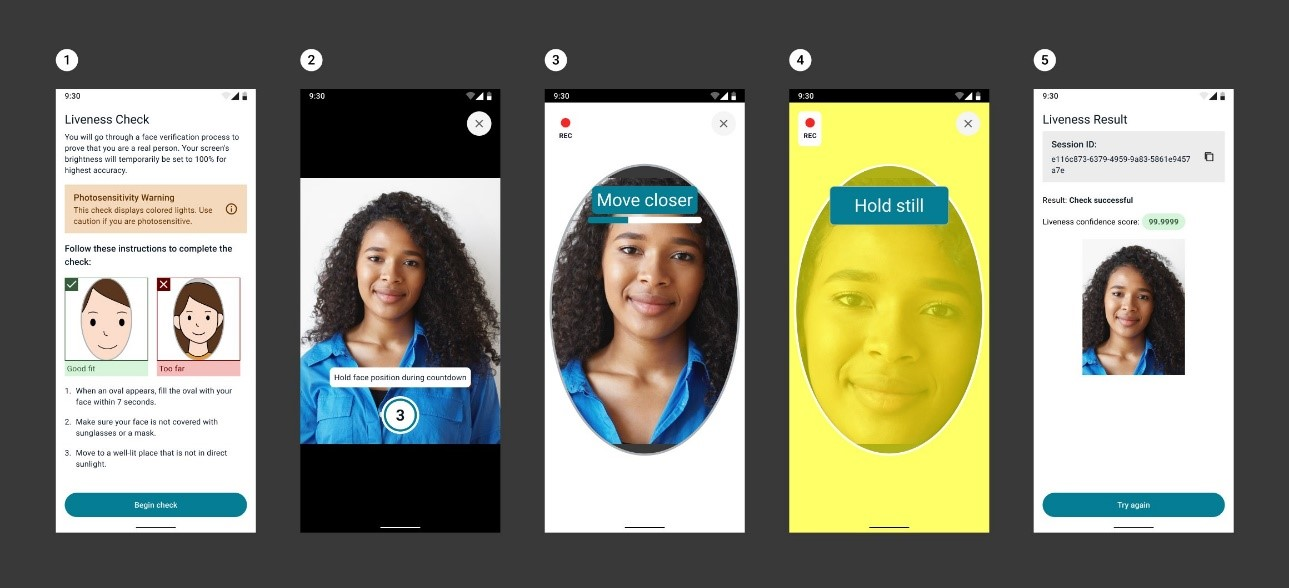
\includegraphics[width=16cm]{figuras/aws_liveness.jpg}
        \caption{Etapas de visualização de tela durante \textit{liveness} desenvolvido pela Amazon.}
        \label{fig:aws_liveness}
\end{figure}

Para assegurar a neutralidade e mitigar vieses discriminatórios, os modelos de ML são treinados com conjuntos de dados (datasets) amplamente diversificados. Essa diversidade abrange variações significativas em tonalidade de pele, faixa etária e identidade de gênero, contribuindo para uma maior equidade na avaliação. \cite{aws_blog_2023}

No mercado de antifraude, a tecnologia encontra diversas aplicações. Em processos de integração digital (\textit{onboarding}), instituições financeiras utilizam a solução para validar a identidade de novos clientes durante a abertura de contas, realizando a comparação biométrica entre a vídeo-selfie e fotografias de documentos oficiais, como carteiras de identidade ou passaportes, frequentemente por meio de interfaces de programação de aplicações (APIs) como a CompareFaces. Adicionalmente, em plataformas de mobilidade urbana, como a Uber, e comércio eletrônico, a tecnologia é implementada para a reautenticação de utilizadores em transações consideradas de alto risco, como transferências bancárias. Setores com restrições etárias, como os de jogos online e tabaco, combinam a detecção de vivacidade com sistemas de estimativa de idade para coibir o acesso de menores. Finalmente, redes sociais e outros serviços digitais empregam esta solução como um substituto avançado para mecanismos de CAPTCHA, exigindo provas de vivacidade para dificultar a proliferação de contas automatizadas (bots) e identidades sintéticas. \cite{aws_rekognition_2023}

\section{Revisão Bibliográfica}
\label{classificação}
O problema a ser estudado neste trabalho, apresentado como classificação de perguntas sobre produtos quanto ao atributo, é definido na literatura como Classificação de Texto (do inglês \textit{Text Classification}). De acordo com a definição apresentada em \cite{survey}, a classificação de texto consiste na seguinte situação: dado um conjunto de instâncias de treino $\mathcal{D} = \{X_1, ..., X_N\}$, onde cada instância $X_i$ é uma sentença textual formada por um conjunto de características (\textit{features}) e está anotada com um valor de classe obtido de um conjunto de k valores discretos indexados como $\{1...k\}$,  treina-se um modelo classificador, que relacionará as características de cada instância de treino a uma das classes. Depois que o treinamento é feito, uma instância de teste, cuja classe é desconhecida, é fornecida ao modelo classificador para que este preveja a classe a qual a instância pertence.

Além de atuar como uma parte integrante de um sistema que responde perguntas de clientes no comércio eletrônico, que é a implementação aqui descrita, a classificação de texto também é muito presente em outros contextos, tais como: obtenção de informações dispostas de forma não estruturada em grandes coleções de documentos \cite{info-retrieval}, filtragem de informações quanto a sua relevância em \textit{streams} de dados \cite{info-filtering}, análise de sentimentos para identificar opinião, sentimento e subjetividade em textos \cite{sentiment-analysis}, sistemas de recomendação que sugerem itens baseados no perfil de interesses do usuário e na descrição do item \cite{recommender-systems}, entre muitos outros \cite{survey2}.

No contexto de resolução de perguntas de clientes reais, a classificação de textos atua para que a pergunta feita seja entendida. Toda pergunta é um questionamento que um cliente possui sobre uma característica de um determinado produto. No contexto deste trabalho, cada classe que o modelo classificador consegue identificar representa uma característica que o produto tem, isto é, representa um atributo do produto. Assim, se um cliente está interessado em saber a marca de uma chave de fenda, ele pergunta "Qual é a marca da chave de fenda?". Esta pergunta, por sua vez, pode ser classificada como uma pergunta sobre o atributo ou classe "marca". Essa forma de responder perguntas encontra diversas dificuldades, que serão discutidas na seção \ref{dificuldades da classificação de perguntas quanto ao atributo}.

\subsection{Detecção de Manipulação de Imagens e Vídeos}
\label{detecção de manipulação de imagens e vídeos}
A crescente sofisticação das ferramentas de edição e geração de imagens e vídeos digitais impulsionou significativamente a necessidade de métodos robustos para a detecção de manipulações. Tais manipulações, que variam desde edições simples até a criação de deepfakes complexos, representam um desafio considerável para a verificação da autenticidade de conteúdo digital, com implicações diretas na disseminação de desinformação e em fraudes. Esta seção aborda as abordagens para a detecção dessas manipulações, iniciando pelas técnicas tradicionais baseadas na identificação de artefatos e inconsistências intrínsecas ao processo de alteração digital.

\subsubsection{Técnicas Tradicionais e Baseadas em Artefatos}

As primeiras abordagens para a detecção de manipulação de imagens frequentemente se concentravam na identificação de anomalias ou "impressões digitais" deixadas pelos processos de edição. Essas técnicas exploram inconsistências que surgem quando um conteúdo digital é alterado, assumindo que o processo de manipulação, por mais sofisticado que seja, introduzirá perturbações detectáveis em relação às características estatísticas de uma imagem autêntica.

\subsubsubsection{Análise de Ruído e Inconsistências Locais}

Um dos pilares da análise forense de imagens digitais é o estudo dos padrões de ruído. Cada dispositivo de captura, seja uma câmera digital ou um scanner, introduz um padrão de ruído idiossincrático, parcialmente devido à Não Uniformidade da Resposta do Fotorreceptor (Photo-Response Non-Uniformity - PRNU). Este padrão, quase como uma impressão digital do sensor, pode ser utilizado para verificar a origem de uma imagem ou para detectar regiões que foram inseridas ou alteradas. A lógica subjacente é que uma manipulação, como a junção de partes de imagens distintas (splicing) ou a cópia de uma região para outra dentro da mesma imagem (copy-move), resultará em uma descontinuidade ou inconsistência nos padrões de ruído. O trabalho de Zhou et al. \cite{zhou2018manipulation} ilustra essa abordagem ao propor uma arquitetura de rede neural de duas vias, onde um dos fluxos é especificamente projetado para analisar as características de ruído da imagem. Este "fluxo de ruído" emprega filtros de Modelos Ricos em Esteganálise (Steganalysis Rich Models - SRM) para extrair descritores de ruído local, com o objetivo de identificar discrepâncias entre as regiões autênticas e as potencialmente manipuladas \cite{zhou2018manipulation}. A premissa é que, mesmo que um falsificador tente aplicar técnicas de pós-processamento para suavizar as transições, as estatísticas de ruído da região adulterada raramente corresponderão perfeitamente às da imagem hospedeira \cite{zhou2018manipulation}.

Embora abordagens mais recentes, como a de Wu et al. \cite{wu2023rethinking}, utilizem técnicas avançadas como aprendizado contrastivo e agrupamento não supervisionado, elas ainda se fundamentam no princípio de que características forenses intrínsecas podem discriminar entre conteúdo original e forjado. Métodos tradicionais frequentemente utilizavam algoritmos de agrupamento (clustering) aplicados a características de ruído extraídas manualmente – como o nível de ruído geral da imagem ou padrões específicos do ruído da câmera – para classificar diferentes blocos ou pixels da imagem como pertencentes a regiões genuínas ou manipuladas \cite{wu2023rethinking}. No entanto, a eficácia dessas técnicas que dependem de características artesanais (hand-crafted features) é frequentemente limitada diante da crescente complexidade das manipulações e da aplicação de operações de pós-processamento que visam ocultar os vestígios da fraude \cite{wu2023rethinking}.

\subsubsubsection(Análise de Compressão JPEG)

O formato JPEG é, indiscutivelmente, um dos mais prevalentes para o armazenamento e transmissão de imagens digitais. Seu algoritmo de compressão, baseado na Transformada Discreta de Cosseno (DCT) e em tabelas de quantização, introduz artefatos característicos, como o efeito de blocagem em regiões de baixa frequência e padrões específicos nos coeficientes DCT. Esses artefatos, embora muitas vezes sutis ao olho humano, podem ser explorados para fins forenses. Uma manipulação comum ocorre quando uma imagem já comprimida em JPEG é editada e, subsequentemente, salva novamente no formato JPEG. Este processo, conhecido como dupla compressão JPEG, pode introduzir anomalias e inconsistências nos padrões de compressão que não estariam presentes em uma imagem comprimida uma única vez \cite{zhou2018manipulation}. A detecção dessas assinaturas de dupla compressão tem sido uma linha de investigação forense estabelecida. Wu et al. \cite{wu2023rethinking} mencionam a utilização do ruído de quantização JPEG como uma das características exploradas por métodos de agrupamento para a detecção de falsificações. De forma complementar, o trabalho CAT-Net, referenciado por Wu et al. \cite{wu2023rethinking}, foca na localização de regiões forjadas através da classificação dos coeficientes DCT, que são elementos centrais do processo de compressão JPEG. A análise da consistência desses coeficientes e das tabelas de quantização entre diferentes regiões de uma imagem pode, portanto, revelar áreas que foram submetidas a ciclos de compressão distintos, indicando uma possível manipulação. É importante notar que a robustez destas técnicas pode ser comprometida por operações de pós-processamento que visam atenuar ou remover os vestígios da compressão.

\subsubsubsection{Outras Características Forenses}

Além das assinaturas de ruído e dos artefatos de compressão, um espectro mais amplo de características forenses pode ser empregado para identificar manipulações visuais. Inconsistências na iluminação, como fontes de luz incompatíveis entre diferentes objetos ou pessoas em uma cena, direções de sombras que desafiam a geometria da cena, ou reflexos que não correspondem ao ambiente circundante, são frequentemente investigadas como indícios de adulteração. Similarmente, anomalias na perspectiva, onde objetos inseridos não se alinham corretamente com o ponto de fuga da imagem original, podem denunciar uma montagem.

A análise de textura, conforme detalhado por Filho et al. \cite{filho_etal_texturas}, embora aplicada a imagens médicas, oferece um arcabouço conceitual relevante. Texturas são padrões espaciais que podem ser caracterizados estatisticamente. Uma manipulação pode introduzir uma região com uma textura que destoa do seu entorno ou pode interromper abruptamente um padrão textural preexistente. Medidas como as características de Haralick, que são derivadas de matrizes de coocorrência de níveis de cinza, quantificam propriedades texturais como homogeneidade, contraste, correlação e entropia \cite{filho_etal_texturas}. Por exemplo, o Segundo Momento Angular (SMA), também conhecido como energia, é uma medida da homogeneidade local dos níveis de cinza. Sua fórmula é dada por:
\begin{equation}
SMA = \sum_{i}\sum_{j}P(i,j)^2
\label{eq:sma}
\end{equation}
onde P(i,j) é a entrada da matriz de coocorrência normalizada para os níveis de cinza i e j. Uma imagem ou região homogênea tende a ter poucas transições de níveis de cinza, resultando em uma matriz de coocorrência com poucas entradas de alta magnitude e, consequentemente, um valor de SMA elevado \cite{filho_etal_texturas}. O Contraste, por outro lado, mede a quantidade de variação local e é calculado como:
\begin{equation}
Contraste = \sum_{i}\sum_{j}(i-j)^2 P(i,j)
\label{eq:contraste}
\end{equation}
Valores elevados de contraste indicam uma maior dispersão dos níveis de cinza \cite{filho_etal_texturas}. No contexto forense, a inserção de um objeto de outra imagem pode resultar em uma assinatura textural distinta que pode ser capturada por essas métricas.

Adicionalmente, artefatos visuais nas bordas das regiões manipuladas são frequentemente explorados. Bordas que se apresentam excessivamente nítidas ou, inversamente, borradas de forma não natural em relação ao restante da imagem podem indicar uma colagem. Diferenças abruptas de contraste entre uma região suspeita e seu fundo imediato também são sinais de alerta \cite{zhou2018manipulation}. Outra característica investigada é a consistência dos padrões do Camera Filter Array (CFA). A maioria dos sensores de câmeras digitais utiliza um CFA (como o padrão Bayer) para capturar informações de cor, e o processo de interpolação para reconstruir uma imagem colorida completa (demosaicing) deixa traços específicos. Uma região importada de outra câmera ou gerada sinteticamente pode não exibir os mesmos artefatos de CFA ou pode interromper os padrões existentes na imagem hospedeira \cite{zhou2018manipulation}. Zhou et al. \cite{zhou2018manipulation} destacam que o fluxo RGB de sua rede neural é treinado para identificar justamente esses tipos de artefatos visuais, como as mencionadas fortes diferenças de contraste e bordas não naturais.

Embora estas técnicas tradicionais tenham estabelecido as fundações da detecção de manipulação de imagens, a sua eficácia individual é frequentemente limitada pela crescente complexidade e realismo das manipulações, bem como pelo emprego de contramedidas forenses pelos perpetradores. Esta limitação pavimentou o caminho para o desenvolvimento de abordagens baseadas em aprendizado profundo, que demonstram maior capacidade de adaptação e generalização, e serão o foco da próxima discussão.

\subsection{Dificuldades da Classificação de Perguntas quanto ao Atributo}
\label{dificuldades da classificação de perguntas quanto ao atributo}
Em Novembro de 2022, o Mercado Livre possuía mais de 7000 atributos únicos, usados para descrever produtos de centenas de subcategorias. Considerando essa condição, estar preparado para responder a perguntas sobre o valor de qualquer atributo, seja ele genérico ou específico, é uma tarefa extremamente difícil, pois ela encontra as limitações citadas a seguir.

\begin{itemize}
    \item Generalização para atributos não vistos nos dados de treino: manter uma base de dados com exemplos de perguntas para cada um dos 7000 atributos é uma tarefa dispendiosa em termos financeiros, e impossível de se realizar manualmente. Além disso, novas categorias de produtos são lançadas todos os dias, o que tornaria esse conjunto de dados obsoleto. Por isso, outros trabalhos da literatura usam estratégias avançadas, como a concatenação de camadas de modelos que não são classificadores \cite{aliexpress}. A técnica proposta no trabalho citado melhorou consideravelmente o reconhecimento de atributos nunca vistos entre os dados de treino, ou seja, aprimorou a habilidade de \textit{zero-shot learning}.
    
    \item Perguntas que se referem à compatibilidade entre produtos: no Mercado Livre existem dois atributos genéricos, o \textbf{COMPATIBLE\_BRANDS} e o \textbf{COMPATIBLE\_MODELS}, que geralmente estão presentes em produtos que são acessórios de objetos maiores, como por exemplo rádios automotivos. É muito comum que as perguntas dessas duas classes diferentes tenham uma estrutura sintática parecida, como exemplificado nas Figuras \ref{fig:ex_model} e \ref{fig:ex_brand}.
    
    \begin{figure}[htb]
        \centering
        \color{blue}- Esse controle é compatível com Xbox Series S?
        \caption{Pergunta que seria classificada como COMPATIBLE\_MODELS.}
        \label{fig:ex_model}
    \end{figure}
    
    \begin{figure}[htb]
        \centering
        \color{blue}- É compatível com micro retífica black\&decker?
        \caption{Pergunta que seria classificada como COMPATIBLE\_BRANDS.}
        \label{fig:ex_brand}
    \end{figure}

    É possível perceber que a classe a que cada exemplo das Figuras \ref{fig:ex_model} e \ref{fig:ex_brand} pertence só pode ser avaliada com base em conhecimento de mundo, que permite distinguir marcas de modelos. Para que um algoritmo de Inteligência Artifical consiga fazer essa distinção com maior assertividade, faz-se necessária uma solução mais específica, como um grande Grafo de Conhecimento com relações entre marcas e modelos de produtos, como explorado em \cite{kg}.
    
    \item Atributos que fazem parte de uma categoria, mas não de outras: cada categoria possui sua lista de atributos válidos. Alguns atributos são mais genéricos e fazem parte da maioria das categorias, enquanto alguns atributos são mais específicos, compõem categorias restritas. Isso faz com que existam atributos análogos entre categorias diferentes. 
    
    Um disco de freio pode ter o atributo \textbf{MATERIAL}, mas uma camiseta só pode ter o atributo \textbf{COMPOSITION}. No entanto, não estamos levando em conta a categoria do produto no momento de fazer a classificação, apenas a pergunta. Isso possibilita que uma pergunta sobre essa camiseta seja classificada como \textbf{MATERIAL}, o que deixaria o cliente sem resposta.
    \item Saudações: os clientes frequentemente introduzem palavras extras, como saudações, para estabelecer a cordialidade entre eles e os atendentes. Isso provoca um ruído desnecessário que pode afetar o resultado final, uma vez que esses cumprimentos também serão fornecidos ao modelo classificador se não forem apropriadamente filtrados.
    \item Variações na ortografia: os clientes possuem diferentes níveis de escolaridade e as perguntas são feitas em um contexto virtual, favorável a abreviações. Esses dois fatores permitem com que uma palavra possa ser escrita das mais variadas formas, o que representa um desafio para os \textit{tokenizadores}, descritos na Seção \ref{pré-processamento dos dados}.
    
    \end{itemize}

\section{Etapas da Classificação de Perguntas Quanto ao Atributo}
\label{etapas_classificação}
A construção de um modelo de classificação de perguntas quanto ao atributo, que pode ser formalizada como uma tarefa de classificação de texto, exige a realização de diversas etapas, que serão descritas nas subseções a seguir.

\subsection{Definição das Classes}
Não é possível, de forma manual, criar uma base de dados com instâncias de todos os atributos existentes para se classificar um produto em um dado \textit{marketplace}. Isso acontece porque aos produtos anunciados nos \textit{marketplaces} podem ser atribuídas centenas ou até mesmo milhares de atributos diferentes. Apesar de existirem modelos pré-treinados que conseguem identificar atributos não usados no treinamento, como em \cite{aliexpress}, torna-se importante ter uma base de dados construída em um conjunto conhecido de classes a fim de avaliar um modelo.

A API de Categorias do Mercado Livre\footnote{\url{https://developers.mercadolivre.com.br/pt_br/categorias-e-atributos}} fornece um recurso \textbf{/attributes} que permite encontrar a lista de todos os atributos de uma dada categoria. Além disso, é possível baixar a árvore de categorias do Mercado Livre\footnote{\url{https://developers.mercadolivre.com.br/pt_br/dump-de-categorias}}, que relaciona todas as categorias e seu grau de parentesco entre si. Um modelo classificador generalista idealmente teria como dados de treino exemplos de perguntas com os atributos que aparecem no maior número de categorias possível, ou seja, os mais genéricos.

\subsection{Coleta de Dados}
\label{coleta de dados}
Os dados provavelmente são a parte mais importante de um sistema de aprendizado de máquina. Em contextos mais simplificados, é facilmente possível obter as bases de dados necessárias para resolver um determinado problema, e elas são constituídos de milhares (ou até mesmo milhões) de instâncias \cite{practical_nlp}. No entanto, na maioria dos projetos de Inteligência Artificial acadêmicos ou comerciais é preciso fazer uso de técnicas de coleta de dados.

Fontes como \cite{practical_nlp} agregaram as técnicas mais empregadas para concluir esta etapa:
\begin{itemize}
    \item Usar uma base de dados pública: consiste em pesquisar se existem bases de dados públicas disponíveis que sejam similares e compatíveis com o problema em questão. Agregadores como o Google Datasets\footnote{\url{https://datasetsearch.research.google.com/}} e o HuggingFace\footnote{\url{https://huggingface.co/datasets}} compilam muitas das opções disponíveis.
    
    \item \textit{Data Scraping}: consiste em encontrar uma fonte de dados relevante na Internet e fazer uso de técnicas de \textit{Web Scraping}, ou seja, obter esses dados de forma que não seja por meio de um programa interagindo com uma API (nem por interação humana). Geralmente esse objetivo é atingido escrevendo um programa que se comunica com um servidor Web, faz uma requisição de dados (muitas vezes em forma de arquivos HTML) e então formata aqueles dados para extrair a informação necessária \cite{web_scaping}.
    \item \textit{Product Intervention}: é uma técnica muito usada por grandes empresas da tecnologia. Quando essas empresas implementam modelos de Inteligência Artificial em seus produtos, os modelos raramente existem de forma isolada do restante do produto. Assim, a técnica de \textit{Product Intervention} consiste em trabalhar juntamente com o time de produto para obter cada vez mais dados diretamente dos usuários, a partir do momento em que estes autorizam. Esses dados são informações relacionadas aos comportamentos que cada usuário teve ao usar aquele produto. Isso acontece por exemplo quando um usuário acessa um \textit{site} de compartilhamento de vídeos, e obtém recomendações de novos vídeos para assistir através de um algoritmo que analisou vídeos previamente assistidos pelo mesmo usuário.
    \item Aumento de dados: consiste em explorar propriedades linguísticas para criar novos textos que são sintaticamente similares aos textos previamente existentes na base de dados.
\end{itemize}


\subsection{Anotação de Dados}
Todas as técnicas de coleta de dados abordadas na Seção \ref{coleta de dados}, exceto o uso de uma base de dados pública, geralmente levam à compilação de dados não-anotados, ou seja, cada sentença coletada ainda não teve a sua classe correspondente identificada. Como os modelos a serem avaliados neste projeto são modelos de classificação de texto, essa informação se faz necessária para o seu treinamento \cite{survey}.

A anotação de dados (ou identificação de classes) é uma tarefa cansativa, demorada e repetitiva, que frequentemente exige o trabalho de uma equipe de anotadores. Além disso, nem sempre é possível saber de forma previsível quantos exemplos anotados serão necessários, uma vez que modelos linguísticos eficazes podem ser construídos com base em uma quantidade de exemplos modesta, desde que os dados de treinamento coincidam com a aplicação desejada \cite{effects_of_corpus_size}.

Depois que as classes estejam manualmente identificadas, uma prática comum na área de Ciência de Dados é dividir os exemplos em dois conjuntos: o de Treino e o de Teste. O conjunto de Treino é composto por aqueles exemplos que serão consumidos durante as iterações de treinamento, enquanto o conjunto de Teste é composto por outros exemplos mantidos fora do treinamento, que não influenciarão as propriedades do modelo e servirão para estimar o quão efetivo um modelo é por meio da comparação da previsão com o valor conhecido \cite{data_science_handbook}. Uma intuição inicial habitualmente tida pelos cientistas é separar 80\% dos exemplos para Treino e 20\% dos exemplos para Teste, seguindo o Princípio de Pareto \cite{80_20}.

Frequentemente não é possível saber quais dados seriam mais adequados para Treino e quais dados seriam mais adequados para Teste. Para resolver esse problema, pode ser usada a técnica de Validação Cruzada. Essa técnica consiste em fazer uma sequência de treinamentos em que cada subconjunto dos dados é usado tanto como conjunto de Treino quanto como conjunto de Teste. Os subconjuntos devem possuir a mesma quantidade de instâncias, e a quantidade de iterações é definida pela quantidade de subconjuntos. Ao final, pode se combinar as métricas dos modelos treinados em cada iteração da sequência (por exemplo, tomando a média) para obter uma melhor métrica da performance do modelo global \cite{data_science_handbook}. 

\subsection{Pré-processamento dos Dados}
\label{pre-processamento dos dados}
Os \textit{softwares} de NLP tipicamente analisam texto dividindo-o em palavras (\textit{tokens}) e sentenças \cite{practical_nlp}. Por isso uma subetapa importante do pré-processamento de dados diz respeito a essas divisões. 

Após as divisões, outros passos são frequentemente efetuados por cientistas de dados, a depender da tarefa específica a qual o modelo treinado se dedicará, assim como do domínio do problema. Esses passos são importantes pelo fato de que um grande dicionário dificulta a tarefa de mineração de dados, por exemplo, no caso de redes neurais. Como redes neurais podem ser caras de se treinar, é importante não desperdiçar capacidade computacional \cite{transformers_book}. Alguns passos comuns a esta etapa são:
\label{pré-processamento dos dados}
\begin{itemize}
    \item \textit{Lowercasing}: consiste em converter todas as letras maiúsculas em minúsculas, deixando o texto todo em caixa baixa \cite{practical_nlp}.
    \item Remoção de \textit{stopwords}: consiste em remover todas aquelas palavras que aparecem com grande frequência no decorrer da base de dados, mas que não contribuem para a semântica da sentença, pois não fornecem nenhuma informação adicional. Ao removê-las, é possível focar nas palavras mais importantes. Alguns exemplos são os artigos, determinantes e pronomes, como ``o'', ``a'', ``os'', ``de'', etc. \cite{practical_nlp} \cite{etaiwi2017impact}.
    \item Remoção da pontuação e/ou números: a remoção de todo tipo de pontuação, tais como pontos de interrogação, vírgulas, pontos finais, entre outros, afeta o resultado de qualquer abordagem de processamento de texto, especialmente aquelas que dependem da frequência de ocorrência de palavras e frases \cite{etaiwi2017impact}.
    \item \textit{Stemming}: é o processo de remover sufixos para reduzir uma palavra de forma que todas as variantes daquela palavra podem se representadas da mesma forma (por exemplo, ``carros'' e ``carro'' são ambos reduzidos para ``carro''). Isso é feito seguindo uma série de regras. Algoritmos de \textit{Stemming} são específicos para cada língua e diferem em termos de performance e acurácia \cite{practical_nlp} \cite{etaiwi2017impact}.
    \item \textit{Lemmatization}: possui algumas similaridades com o \textit{Stemming}, porém consiste em mapear todas as diferentes formas de uma palavra para a sua palavra base. Por exemplo, o adjetivo ``melhor'' se torna ``bom''. Esse processo requer um conhecimento linguístico maior do que o anterior \cite{practical_nlp}.
\end{itemize}


\subsection{Transformação dos Dados}
Para que algoritmos de aprendizado de máquina trabalhem com dados textuais, esses dados devem ser convertidos para uma representação numérica. Se textos são representados como vetores de números, a representação numérica é chamada de \textit{Vector Space Model} (VSM). Diversas abordagens algébricas podem ser feitas para se obter um VSM \cite{practical_nlp}. Elas serão elaboradas nas Seções \ref{bag of words e tf-idf} e \ref{tokenizadores}.

\subsubsection{Bag of Words e TF-IDF}
\label{bag of words e tf-idf}
Duas abordagens clássicas de representação de dados textuais são a \textit{Bag of Words} e a TF-IDF. Essas abordagens são antigas e de relativa fácil implementação, o que faz com que sejam frequentemente consideradas como linhas de base em artigos científicos. Uma referência inicial a \textit{Bag of Words} em um contexto linguístico está em \cite{bag-of-wordsPaper}, onde o autor argumenta que ``língua não é simplesmente uma \textit{bag of words}, mas sim uma ferramenta com propriedades particulares que foram forjadas durante seu uso''. Já a definição da abordagem TF-IDF está em \cite{tf-idfPaper}, onde a autora argumenta que ``termos devem ser ponderados de acordo com a frequência em que aparecem no conjunto''. Logo, em um contexto onde é feita uma pesquisa usando palavras-chave para encontrar documentos relacionados, a correspondência com termos mais específicos é de maior valor do que a correspondência com termos mais frequentes.

A representação de instâncias usando a abordagem \textit{Bag of Words} pode utilizar o formato de uma tabela atributo-valor, onde cada documento $d_i$ é um exemplo da tabela e cada termo (palavra) $t_j$ é um elemento do conjunto de atributos \cite{bag_of_words}.

\begin{center}
\begin{table}[ht]
\caption{Representação de documentos}
\label{table:representação de documentos}
\centering
    \begin{tabular}{|c | c | c | c | c || c|} 
     \hline
      & $t_1$ & $t_2$ & ... & $t_M$ & $C$ \\ [0.5ex] 
     \hline
     $d_1$ & $a_{11}$ & $a_{12}$ & ... & $a_{1M}$ & $c_1$ \\ 
     \hline
     $d_2$ & $a_{21}$ & $a_{22}$ & ... & $a_{2M}$ & $c_2$ \\
     \hline
     ... & ... & ... & ... & ... & ... \\
     \hline
     $d_N$ & $a_{N1}$ & $a_{N2}$ & ... & $a_{NM}$ & $c_N$ \\
     \hline
    \end{tabular}
\end{table}
\end{center}

Cada documento $d_i$ da Tabela \ref{table:representação de documentos} é um vetor $d_i = (a_{i1}, a_{i2}, ..., a_{iM})$, no qual o valor $a_{ij}$ refere-se ao valor associado ao j-ésimo termo do documento $i$. Esse valor pode ser calculado usando diferentes medidas. Se usarmos a medida \textit{tf}, por exemplo, o valor de $a_{ij}$ será a frequência que o termo $t_j$ aparece no documento $d_i$. No entanto, quando algumas palavras aparecem na maioria dos documentos, eles podem não fornecer informações úteis \cite{bag_of_words}.

A TF-IDF (\textit{term frequency–inverse document frequency}) é outra abordagem de ponderação de termos. Considere $T = \{t_1, ..., t_n\}$ como sendo o conjunto de todos os termos que aparecem em todos os documentos da base de dados. Então, um documento $d_i$ é representado por um vetor de valores reais de $n$ dimensões dado por $x_i = (x_{i1}, ..., x_{in})$ com um componente para cada possível termo do conjunto T \cite{tf-idf}. O peso $x_{ij}$ correspondente ao termo $t_j$ do documento $d_i$ é geralmente um produto de três partes: uma que depende da frequência de $t_j$ em $d_i$, uma que depende da frequência de $t_j$ no conjunto de documentos como um todo, e uma parte de normalização que depende de $d_j$. A fórmula mais comum para a ponderação TF-IDF é definida pela Equação \ref{eq_tfidf}, onde $TF_{ij}$ é a frequência do termo (isto é, o número de ocorrências) de $t_j$ em $d_i$; $IDF_{j}$ é o IDF de $t_j$, definido como o $\log{\frac{N}{DF_j}}$, onde $N$ é o número total de documentos; e $DF_j$ é o número de documentos onde $t_j$ aparece \cite{tf-idf}.

\begin{equation}\label{eq_tfidf}
        x_{ij} = TF_i \cdot IDF_j \cdot (\sum_j(TF_{ij}IDF_{j})^2)^{-1/2}
\end{equation}

\subsubsection{Tokenizadores}
\label{tokenizadores}
Os Tokenizadores são formas de representação de dados textuais mais recentes, que representam o atual estado da arte. Mais uma vez, a cada unidade em que se divide o texto uma representação numérica relacionada é gerada. 

É possível tokenizar em relação a caracteres ou a palavras, mas a forma mais habitual de tokenização empregada pelos cientistas de dados atualmente é a \textit{Subword Tokenization}. Ela combina os melhores aspectos das tokenizações por palavras ou caracteres. Por um lado, é desejável que palavras raras sejam divididas em partes menores, o que permite que o modelo lide com palavras complexas e/ou escritas incorretamente. Por outro lado, é desejável que palavras frequentes sejam mapeadas como entidades únicas para que seja possível manter o comprimento da entrada do modelo em um tamanho controlável \cite{transformers_book}. 

O Tokenizador usado por modelos Transformadores, como os que serão descritos na Seção \ref{modelos ou algoritmos classificadores de texto}, é o WordPiece \cite{wordpiece1} \cite{wordpiece2}, apresentado pelo Google como um dos componentes do seu modelo BERT, aplicado neste trabalho. Ao oferecer como exemplo a sentença ``Tokenizing text is a core task of NLP'' ao \textit{framework} Transformers \cite{hf_transformers_paper}, que implementa o WordPiece, é feita a tokenização. Na prática, trechos de palavras são mapeados a números inteiros. A Figura \ref{fig:input_ids} mostra esse mapeamento.

\begin{figure}[htb]
        \centering
        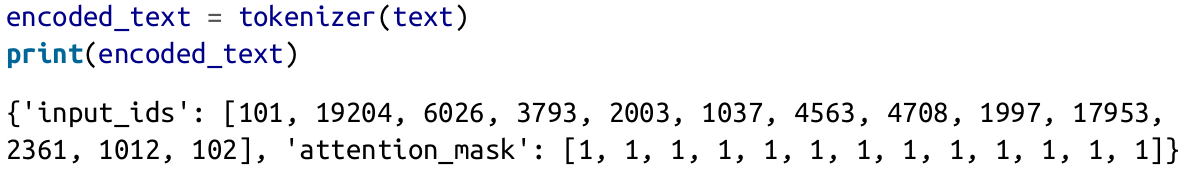
\includegraphics[width=14cm]{figuras/input_ids.png}
        \caption{Mapeamento de \textit{subtokens} a números inteiros únicos. Fonte: \cite{transformers_book}}
        \label{fig:input_ids}
\end{figure}

Ao converter os números inteiros para tokens, como mostrado na Figura \ref{fig:tokens}, é possível entender como as palavras são divididas. Dois tokens especiais, o [CLS] e o [SEP], foram adicionados ao início e ao fim da sentença. Além disso, as palavras passaram por \textit{lowercasing}, subetapa de pré-processamento explicada em \ref{pre-processamento dos dados}. Outro detalhe que se pode observar é que ``tokenizing'' e ``NLP'' foram divididas em dois tokens. Isso faz sentido, uma vez que uma das premissas desse tokenizador é dividir palavras raras em unidades menores \cite{transformers_book}.

\begin{figure}[htb]
        \centering
        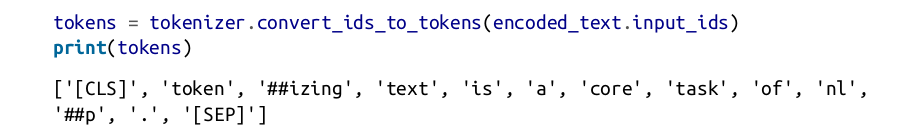
\includegraphics[width=14cm]{figuras/tokens.png}
        \caption{Resultado da conversão de números inteiros únicos para tokens. Fonte: \cite{transformers_book}}
        \label{fig:tokens}
\end{figure}

\subsection{Algoritmos Classificadores de Texto}
\label{modelos ou algoritmos classificadores de texto}
A tarefa de classificação de textos é estudada desde muito tempo, e portanto, diversos métodos de cumpri-la foram implementados ao longo dos anos. \citeonline{survey} e \citeonline{survey2} compilaram em suas pesquisas diversas técnicas de aprendizado de máquina para classificação de texto, tais como: algoritmo de Rocchio \cite{rocchio}; \textit{boosting} \cite{boosting} e \textit{bagging} \cite{bagging}, que são algoritmos de votação; regressão logística \cite{logistic_regression}; Naïve Bayes \cite{naive_bayes}; \textit{k-nearest neighbor} \cite{k_nearest}; \textit{support vector machines} (SVMs) \cite{svm}; árvores de decisão \cite{decision_tree} e \textit{random forests} \cite{random_forests}; algoritmos baseados em redes neurais; dentre muitos outros.

No entanto, este trabalho se dedica a explorar algumas das técnicas mais recentes de classificação de texto, especificamente as que são baseadas em \textit{Deep Learning}. \citeonline{survey3} compilaram em sua pesquisa diversas dessas técnicas, tais como: \textit{transformers} \cite{attention_is_all_you_need} ou \textit{pre-trained language models}; \textit{feed-forward networks}, como por exemplo o modelo DAN \cite{dan}; modelos baseados em RNNs, como o MT-LSTM \cite{mt-lstm}; modelos baseados em CNNs, como o modelo DCNN \cite{dcnn}; \textit{memory-augmented networks}, como a NSE \cite{nse}; dentre muitos outros. Dentre elas, duas arquiteturas diferentes de Transformadores foram escolhidas para esse projeto, BERT e DIETClassifier.

\subsubsection{BERT}
\label{bert_subsubsection}
O BERT é um modelo de Transformador \cite{attention_is_all_you_need}, e foi apresentado em \cite{bert}. Transformadores são algoritmos de \textit{Deep Learning} que possuem como diferencial os mecanismos de auto-atenção, cujo desenvolvimento é explicado em ordem cronológica nos parágrafos seguintes.

Há alguns anos, era comum que tarefas como a tradução fossem resolvidas usando a arquitetura \textit{encoder}-\textit{decoder}. Isto é, uma frase qualquer em Inglês era convertida para uma representação vetorial, chamada de \textit{last hidden state}, dentro de uma arquitetura chamada de \textit{encoder}, composta de redes neurais recorrentes (RNNs). Na outra ponta, essa representação vetorial era convertida de volta para uma outra língua, como o Alemão, na arquitetura conhecida como \textit{decoder}, feita também de RNNs. Porém, essa solução trazia um problema: a representação vetorial tinha dimensões fixas, o que fazia com que informações fossem perdidas em longas sentenças \cite{transformers_book}. Essa solução era aplicada antes do advento dos mecanismos de atenção.

Os mecanismos de atenção vieram como uma solução para esse problema de perda de informação. A Figura \ref{fig:decoder_attention} retrata como funciona uma iteração desses mecanismos. Com eles, ao invés de produzir uma única representação vetorial para a frase em Inglês, o \textit{encoder} produz uma representação vetorial diferente para cada palavra da frase. Ao final do Passo 1, todas as representações vetoriais são enviadas para o \textit{decoder}. Após receber as representações, o \textit{decoder} fornece para cada uma delas uma pontuação no Passo 2. Essa pontuação, que é um número inteiro simples, é fornecida como entrada para a função softmax(), que por sua vez é uma função que transforma um vetor de números em uma distribuição de probabilidades, onde o maior elemento do vetor recebe um grande peso (observe a probabilidade associada a cada elemento no Passo 3 da Figura \ref{fig:decoder_attention}). A função softmax() é descrita pela Equação da Figura \ref{eq_softmax}. Finalmente, no Passo 4, cada representação vetorial é multiplicada pelo seu valor de softmax(), o que faz com que representações vetoriais que tinham grandes pontuações no Passo 2 sejam amplificadas, em detrimento das representações vetoriais que tinham baixas pontuações \cite{attention_explained} \cite{attention_paper1} \cite{attention_paper2}.

\begin{figure}[h!t]
  \centering 
    $\text{softmax}(x_i) = \dfrac{\exp(x_i)}{\sum_j \exp(x_j)}$
    \caption{A softmax() de um elemento de um vetor é a exponencial desse elemento de vetor dividida pela soma das exponenciais de todos os elementos do vetor.}
    \label{eq_softmax}
\end{figure}    

\begin{figure}[htb]
        \centering
        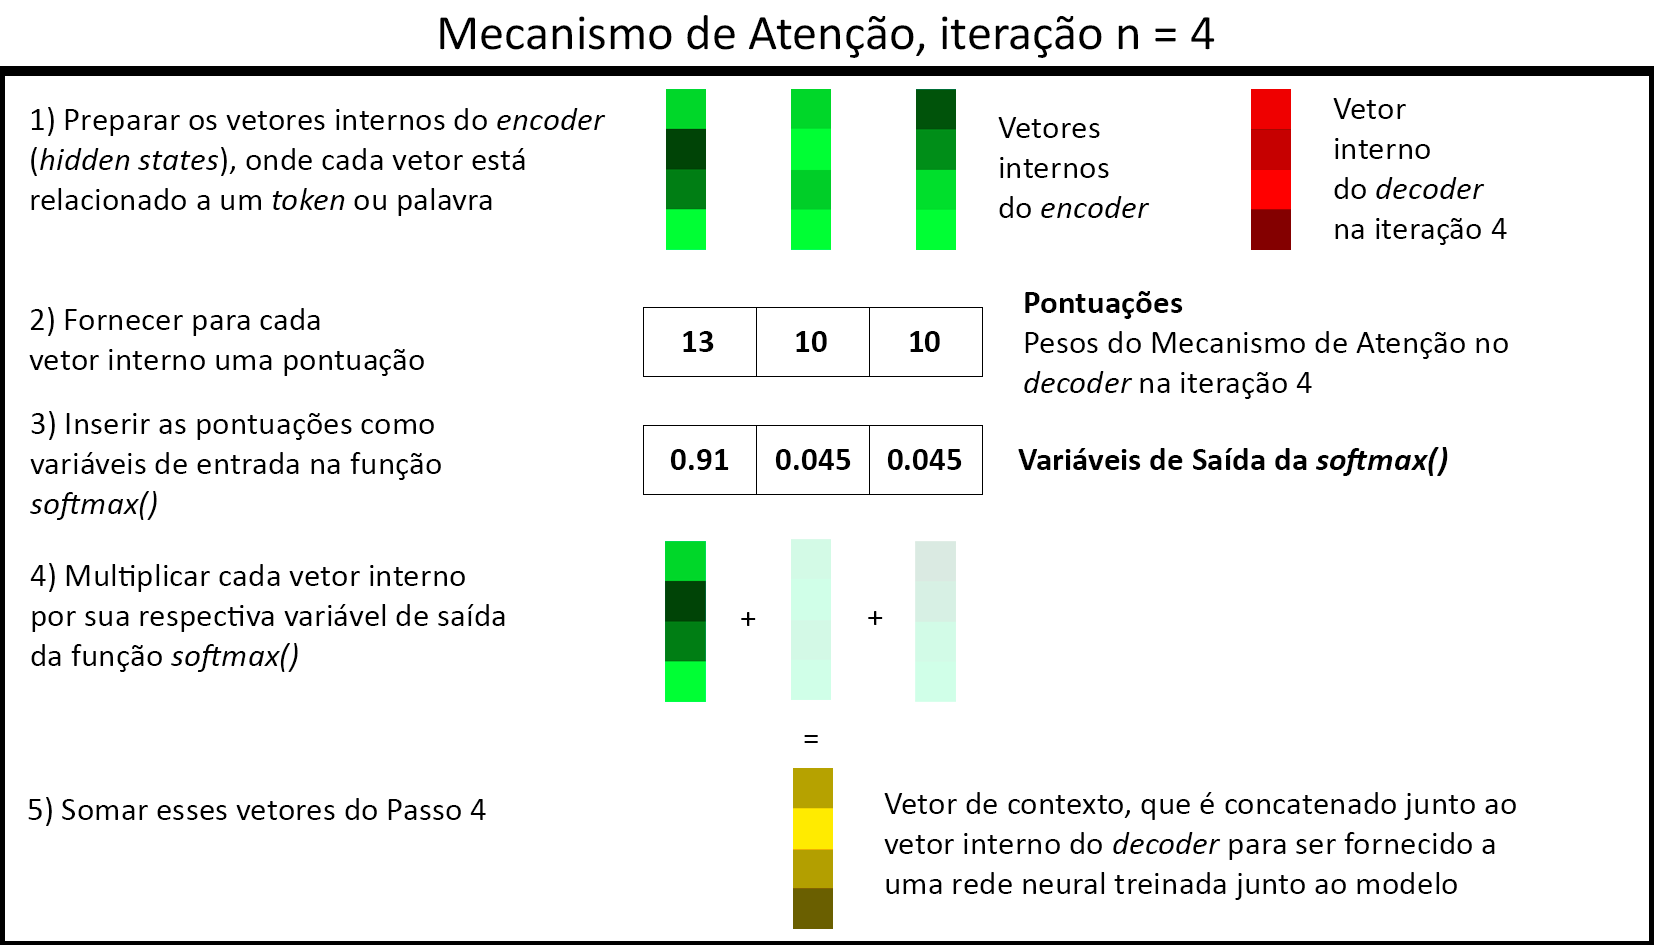
\includegraphics[width=14cm]{figuras/mecanismo_de_atencao.png}
        \caption{Mecanismo de atenção em um \textit{decoder}. Fonte: \cite{attention_explained}}
        \label{fig:decoder_attention}
    \end{figure}

Os mecanismos de Auto-atenção são uma evolução dos mecanismos de Atenção, e foram apresentados como uma característica dos Transformadores. A principal ideia por trás deles é que, ao invés de usar uma representação vetorial fixa para cada \textit{token}, eles usam a sequência inteira para calcular uma média ponderada de cada representação vetorial \cite{transformers_book}. Dessa forma, quando uma sentença possui a palavra ``manga'', por exemplo, é possível diferenciar pelo contexto se a sentença se refere à fruta ou à parte da camisa, e assim produzir uma representação vetorial que leva em consideração esse significado.

A Tabela \ref{tab:attentions} compila os principais pontos dos mecanismos referenciados nos três parágrafos anteriores: pré-atenção (o que era aplicado antes do avento dos mecanismos de atenção), Atenção, e Auto-atenção. Ela considera uma tarefa de tradução de sentenças, onde o Codificador (\textit{encoder}) recebeu uma sentença em Inglês, por exemplo, e o Decodificador (\textit{decoder}) deve fornecer como saída a tradução da sentença em Português. 

\begin{table}[htb]
\centering
\caption{Os três mecanismos: pré-atenção, Atenção e Auto-atenção}
\begin{tabular}{|p{5cm}|p{10cm}|}
\hline
Mecanismo & Principais Pontos \\
\hline
Pré-atenção & O Decodificador tem acesso a apenas um dos vetores (hidden states) gerados pelo Codificador, e esse vetor possui tamanho fixo. Isso faz com que tanto frases simples quanto textos longos sejam representados por um vetor de mesmo tamanho, o que faz muitas informações serem perdidas quando usando textos longos. \\
\hline
Atenção (Attention) & O Decodificador tem acesso a todos os vetores (hidden states) gerados pelo Codificador. Esses vetores são gerados sequencialmente, ou seja, um a cada palavra. Isso significa que na iteração 3, por exemplo, existem três vetores. O Mecanismo de Atenção consiste em fornecer um peso para cada um desses vetores para assim saber quais vetores merecem mais foco, ou mais atenção, a cada iteração. A vantagem é que se torna possível representar adequadamente textos longos, assim como se torna possível criar uma associação entre as palavras ``casa'' e ``house'', por exemplo, mesmo que ``casa'' seja a primeira palavra da frase em Português e ``house'' seja a última palavra da frase em Inglês. \\
\hline
Auto-atenção/Transformadores (Self-attention/Transformers) & Os pesos dos vetores que definem cada palavra são aprendidos levando em consideração apenas o Codificador. A vantagem é que isso permite obter vetores contextualizados - isto é, obter um vetor diferente para ``manga'', a fruta, do vetor que seria gerado para ``manga'', a parte da camisa. Esse aprendizado é feito ponderando outras palavras do contexto daquela sentença. \\
\hline
\end{tabular}
\label{tab:attentions}
\end{table}

O BERT, sigla para \textit{``Bidirectional Encoder Representations from Transformers''}, se destaca entre os demais Transformadores pelo fato de criar representações vetoriais profundas bidirecionais, isto é, considerando o contexto à esquerda e o contexto à direita de uma determinada palavra \cite{bert}. Para isso, ele usa apenas o \textit{encoder} da arquitetura dos Transformadores, e é pré-treinado em bases de dados extensas: o \textit{BookCorpus} \cite{bookcorpus_paper} e a \textit{Wikipedia}\footnote{\url{https://en.wikipedia.org/}} em inglês. Essas representações foram aprendidas de forma bidirecional automaticamente ao fornecer uma base de dados de Treino composta em 80\% por sentenças com palavras aleatoriamente deixadas em branco (chamadas de palavras mascaradas em \citeonline{bert}), como ilustra a Figura \ref{fig:ex_mlm}. Isso fez com que o modelo se tornasse assertivo em predizer qual palavra melhor completaria o espaço em branco fornecido. No exemplo da Figura \ref{fig:ex_mlm}, ao considerar ``Eu estou'' de um lado e ``sorvete'' do outro, as opções se tornam restritas: se restringem a palavras como ``tomando'', ``comendo'', ``lambendo''. Não seria possível ter tamanha assertividade na resposta se o modelo considerasse apenas ``Eu estou'' e tentasse predizer a palavra restante.

\begin{figure}[htb]
    \centering
    \color{blue}Eu estou tomando sorvete$\rightarrow$ Eu estou \_\_\_\_ sorvete
    \caption{Como os criadores do modelo BERT tinham a intenção de que ele aprendesse a considerar tanto palavras que estão ao início de uma sentença quanto palavras que estão ao final de uma sentença, para que assim as representações vetoriais das palavras levassem em conta o contexto, 80\% da base de dados de Treino era composta de sentenças com palavras mascaradas, isto é, em branco.}
    \label{fig:ex_mlm}
\end{figure}

Um fator que tornou o BERT muito popular foi a praticidade de sofrer \textit{fine-tuning}, isto é, de receber uma camada de saída a mais e ter a possibilidade de ajustar apenas os pesos dela: isso tornou o modelo eficiente em muitas outras tarefas específicas, como classificação de texto. O BERT ajudou a definir o estado da arte, e por isso foi precursor de vários modelos frequentemente usados nos dias atuais, como os modelos RoBERTa \cite{roberta_paper} \cite{transformers_book}.

\subsubsection{DIETClassifier}
O DIETClassifier \cite{diet_classifier} também é um modelo de Transformador \cite{attention_is_all_you_need}. Sua característica mais marcante é o fato dele possibilitar que duas tarefas sejam executadas ao mesmo tempo sobre uma entrada de texto: ele faz classificação de intenções e reconhecimento de entidades na mesma iteração, normalmente associadas a uma interface de conversação usuário-máquina, como mostra a Figura \ref{fig:diet_schema}. Enquanto a classificação de intenções se assemelha muito à tarefa de classificação de texto abordada aqui, e está relacionada a entender qual objetivo o usuário tinha ao enviar uma determinada frase, o reconhecimento de entidades busca categorizar palavras específicas da sentença em classes previamente vistas pelo modelo \cite{diet_blog}.

\begin{figure}[htb]
        \centering
        \includegraphics[width=14cm]{figuras/tarefas_do_DIET.png}
        \caption{As duas tarefas que são executadas ao mesmo tempo por um classificador DIET: classificação de intenções e reconhecimento de entidades.}
        \label{fig:diet_schema}
\end{figure}

Outros pontos importantes levantados pelos autores do DIETClassifier são a sua arquitetura modular e seus bons resultados comparados a modelos pré-treinados, como o BERT. A modularização se dá porque é possível usar as representações vetoriais aprendidas por modelos como o próprio BERT como uma de suas camadas, e mesmo assim montar uma arquitetura completa que tenha o classificador DIET como camada de saída. Os bons resultados se devem ao fato de que arquiteturas montadas com o DIET podem ter resultados tão bons quanto os demonstrados por modelos maiores, e mesmo assim chegam a ser até 6x mais rápidas de se treinar \cite{diet_classifier} \cite{diet_blog}.

\subsection{Métricas de Desempenho}
\label{métricas_de_desempenho}
As matrizes de confusão são um tipo de visualização que permite entender as nuances do desempenho dos modelos treinados, classe por classe. Nesse tipo de gráfico, as linhas representam as classes verdadeiras, enquanto as colunas representam as classes previstas pelo modelo em questão (a representação em linha ou coluna varia entre trabalhos). 

Suponha que um problema de Processamento de Linguagem Natural foi apresentado, onde um modelo de Inteligência Artificial foi treinado para classificar avaliações dos usuários sobre um determinado filme em \textbf{Bom}, \textbf{Razoável} e \textbf{Ruim}. Esse modelo obteve o resultado retratado na matriz de confusão da Figura \ref{fig:cm_example}. Ao olhar o termo da primeira coluna com a primeira linha, percebe-se que 3 avaliações \textbf{Bom} foram classificadas como \textbf{Bom} pelo modelo treinado. Por outro lado, ao olhar o termo ao lado vê-se que 4 avaliações \textbf{Bom} foram classificadas como \textbf{Razoável} pelo modelo treinado, o que está incorreto.   Dessa forma, um modelo que consegue prever corretamente a opinião dos espectadores em cada avaliação em todas as avaliações de um determinado conjunto teria uma matriz de confusão diagonal (os únicos termos diferentes de zero seriam aqueles da diagonal principal) \cite{metrics_survey}.

\begin{figure}[htb]
        \centering
        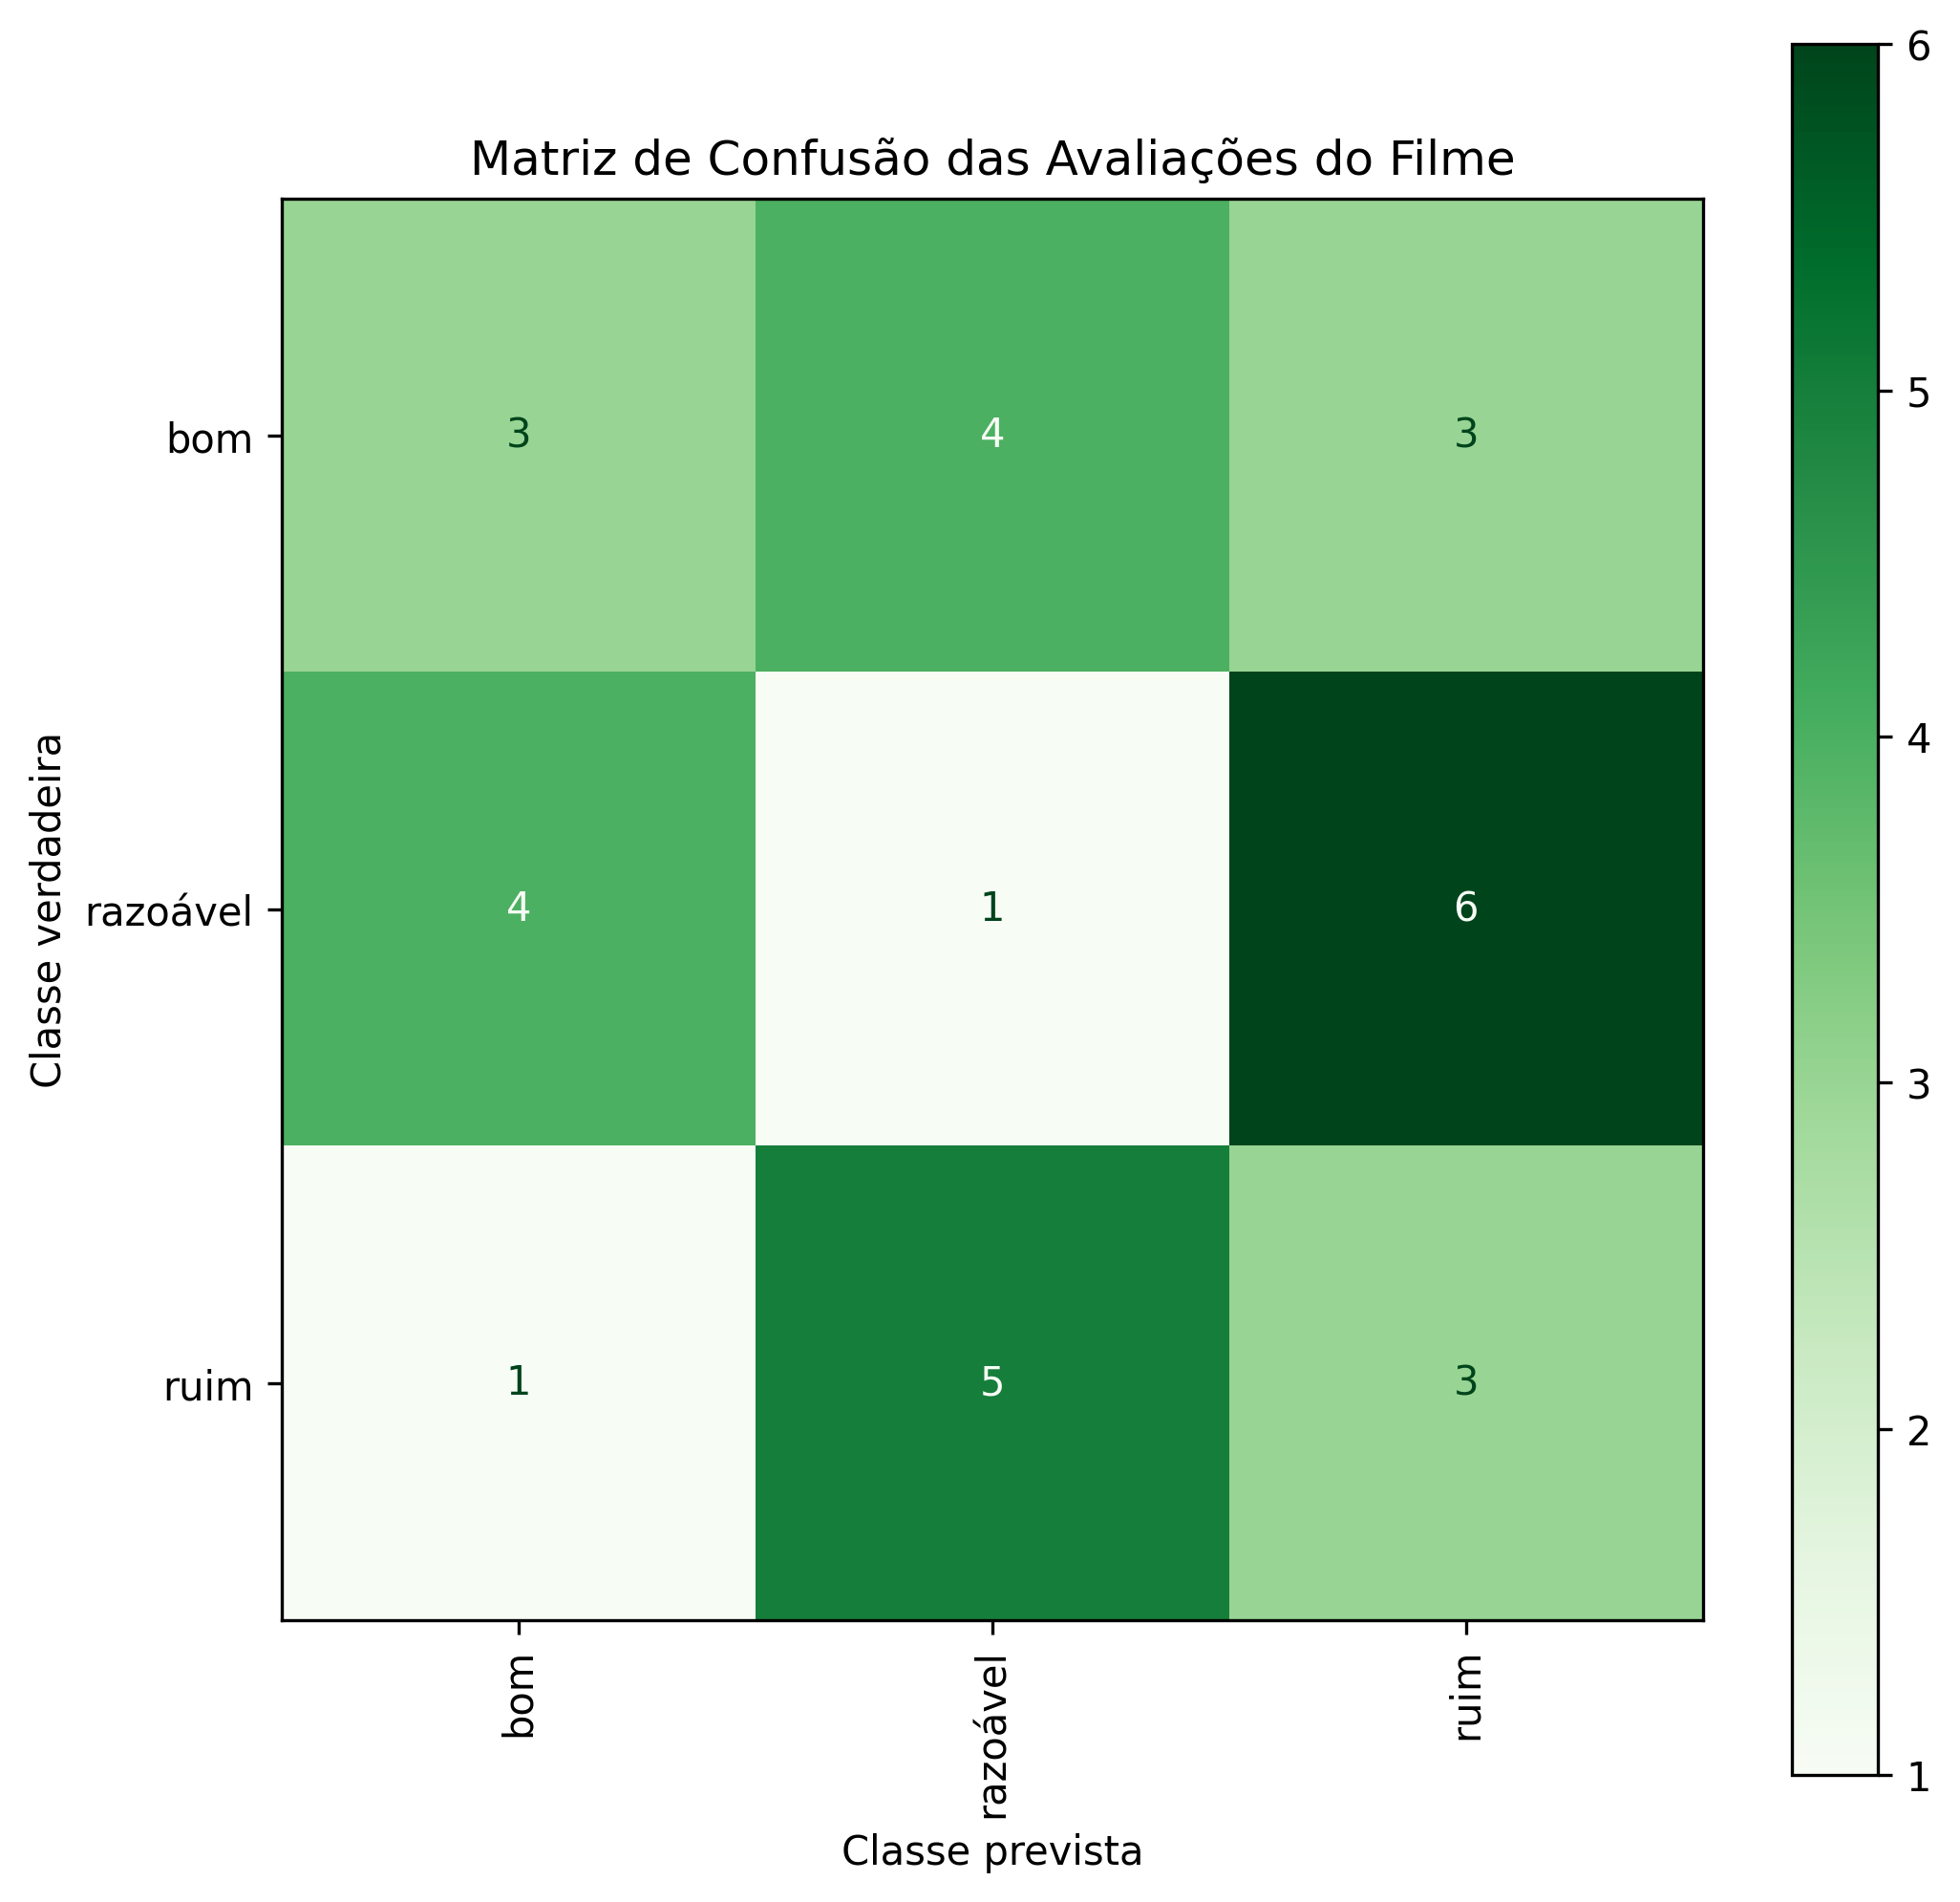
\includegraphics[width=14cm]{figuras/exemplo_filmes.png}
        \caption{Exemplo de visualização de Matriz de Confusão, que será esmiuçado em seções posteriores.}
        \label{fig:cm_example}
\end{figure}

Soluções para problemas de classificação multi-classe, como o abordado neste trabalho, devem ser avaliadas por um conjunto de métricas específico. Trabalhos como a \textit{survey} conduzida em \cite{metrics_survey} se dedicaram a levantar as características dos indicadores de desempenho mais comuns para esse tipo de tarefa, o que é fundamental para a comparação entre os desempenhos dos diferentes modelos treinados. Algumas métricas permitem avaliar a predição de exemplos como um todo. Outras métricas permitem avaliar o quão boa é a predição de uma determinada classe em comparação com outras classes. O engenheiro de aprendizado de máquina deve entender qual tipo de resultado é mais importante e escolher as métricas adequadas se baseando nisso. Entre as métricas mais conhecidas pela literatura, estão:

\begin{itemize}
    \item \textbf{Acurácia}: reflete o quão próximo um dado conjunto de observações (ou previsões, no contexto de Inteligência Artificial) está próximo dos seus valores verdadeiros. Ela considera a soma de todos os elementos classificados corretamente no numerador, enquanto o denominador soma os elementos classificados corretamente com os classificados incorretamente. Assume valores entre 0 e 1 \cite{metrics_survey}.
    \begin{equation}\label{eq_accuracy}
        \text{Acurácia} = \dfrac{TP + TN}{TP + TN + FP + FN}
    \end{equation}
    Na fórmula de Acurácia:
        \begin{itemize}
            \item TP: \textit{true positives}, ou verdadeiros positivos, que é quando um exemplo da classe Positiva é classificado como um elemento da classe Positiva.
            \item TN: \textit{true negatives}, ou verdadeiros negativos, que é quando um exemplo da classe Negativa não é classificado como um elemento da classe Positiva.
            \item FP: \textit{false positives}, ou falsos positivos, que é quando um exemplo da classe Negativa é classificado como um elemento da classe Positiva.
            \item FN: \textit{false negatives}, ou falsos negativos, que é quando um exemplo da classe Positiva é classificado como um elemento da classe Negativa.
        \end{itemize}
    A Acurácia é calculada sobre todo o conjunto avaliado, considerando os exemplos de todas as classes. Existem classes com mais exemplos e classes com menos exemplos. Isso indica que classes mais populadas terão um maior peso em comparação com as classes menos populadas no valor de Acurácia \cite{metrics_survey}.
    \item \textbf{Precisão}: é a proporção de exemplos que o modelo previu como pertencentes à classe Positiva que realmente são daquela classe, ou seja, ela representa o quanto é possível confiar em um modelo quando ele prevê que um exemplo é de uma dada classe. É uma métrica dada para cada uma das classes no contexto de classificação multi-classes. Assume valores entre 0 e 1 \cite{metrics_survey}. A Precisão de uma classe $k$ será igual a (Eq. \ref{eq_precision}):
    \begin{equation}\label{eq_precision}
        \text{Precisão}_k = \dfrac{TP_k}{TP_k + FP_k}
    \end{equation}
    Ao final, caso seja preciso obter uma métrica de Precisão generalizada para todas as classes, pode-se fazer uma média ponderada considerando cada valor encontrado na (Eq. \ref{eq_precision}), o que tira o efeito do desbalanceamento no número de exemplos entre as classes \cite{sk}.
    \item \textbf{Revocação}: considerando todos os exemplos que a classe Positiva possui, indica a porcentagem de quantos foram corretamente identificados como pertencentes a essa classe. É uma métrica dada para cada uma das classes no contexto de classificação multi-classes. Assume valores entre 0 e 1 \cite{metrics_survey}. A Revocação de uma classe $k$ será igual a (Eq. \ref{eq_recall}):
    \begin{equation}\label{eq_recall}
        \text{Revocação}_k = \dfrac{TP_k}{TP_k + FN_k}
    \end{equation}
    Ao final, caso seja preciso obter uma métrica de Revocação generalizada para todas as classes, pode-se fazer uma média ponderada considerando cada valor encontrado na (Eq. \ref{eq_recall}), o que tira o efeito do desbalanceamento no número de exemplos entre as classes \cite{sk}.
    \item \textbf{\textit{F1-Score}}: é uma métrica que agrega as métricas de Precisão e Revocação em uma fórmula de média harmônica. Assim, torna-se possível encontrar a melhor relação entre as duas quantidades. É uma métrica dada para cada uma das classes no contexto de classificação multi-classes. Assume valores entre 0 e 1 \cite{metrics_survey}. O \textit{F1-Score} de uma classe $k$ será igual a (Eq. \ref{eq_f1}):
    \begin{equation}\label{eq_f1}
        {F1}_k = 2\cdot\dfrac{\text{precisão} \cdot \text{revocação}}{\text{precisão} + \text{revocação}}
    \end{equation}
    Ao final, caso seja preciso obter uma métrica de \textit{F1-Score} generalizada para todas as classes, pode-se fazer uma média ponderada considerando cada valor encontrado na (Eq. \ref{eq_f1}), o que tira o efeito do desbalanceamento no número de exemplos entre as classes \cite{sk}.
\end{itemize}

\section{Trabalhos Relacionados}
\label{relacionados}
O estudo da implementação de modelos de aprendizado de máquina para Classificação de Texto é amplo, distribuído entre diferentes tipos de aplicações pelo mundo todo. Alguns dos muitos trabalhos nesse campo se assemelham com o trabalho apresentado por também estarem no contexto do \textit{e-commerce}, enquanto outros são similares porque sua base de dados também é composta por exemplos em Português \cite{survey}. 

Em \cite{relacionado_pt}, o autor usa uma base de dados em Português para classificar perguntas sobre conhecimentos gerais em relação à classe daquela pergunta, como Localidade, Pessoa, etc. Ele então combina essa técnica com reconhecimento de entidades e recuperação da informação para percorrer milhares de documentos e obter a resposta. O pré-processamento é feito a partir de \textit{Lowercasing} e do uso dos algoritmos TF-IDF e \textit{Word2Vec} \cite{word2vec} individualmente ou em conjunto (chamado pelo autor de Híbrido). Três arquiteturas de aprendizado de máquina são treinadas e comparadas com outras mais simples: \textit{Support Vector Machine} (SVM), \textit{Perceptron} Multicamadas (MLP) e \textit{Long Short-Term Memory} (LSTM) de 4 camadas. A avaliação da Classificação de Perguntas foi feita usando Validação Cruzada (\textit{Cross-validation}) e alterando o tamanho da base de dados, assim como empregando métricas como Precisão, Revocação e \textit{F1-Score}. Além disso, houve a criação de matrizes de confusão para comparar o desempenho dos diferentes algoritmos de pré-processamento (\textit{Bag of Words}, TF-IDF, \textit{Word2Vec} e Híbrido, ou seja, TF-IDF e \textit{Word2Vec} em conjunto) para cada arquitetura de aprendizado de máquina (SVM, MLP e LSTM). Entre os resultados encontrados pelo trabalho está o de que o pré-processamento Híbrido na etapa de classificação de perguntas, usando os algoritmos TF-IDF e \textit{Word2Vec} em conjunto, levou a uma melhor classificação das perguntas do que o pré-processamento individual. Outro resultado encontrado foi o de que a etapa de classificação de perguntas foi importante para o desempenho geral do sistema completo (classificação de perguntas e, após, recuperação da informação).

Uma aplicação da Classificação de Texto voltada para o campo de avaliações de produtos, um espaço comum em sites de comércio \textit{online}, é abordada em \cite{relacionado_tur}. Usando uma base de dados com exemplos em Turco, os autores usaram oito diferentes algoritmos de aprendizado de máquina para classificar não apenas o sentimento do cliente em relação à experiência da compra, mas também aspectos sobre a entrega ser rápida ou se o avaliador recomenda que futuros compradores peçam tamanhos menores. Assim, eles analisaram avaliações de clientes de uma forma orientada a aspectos, e quatro formas de representação vetorial (TF-IDF, \textit{Word2Vec}, \textit{GloVe} \cite{glove} e BERT) foram usadas para treinar oito métodos de classificação (\textit{Random Forest} (RF), \textit{Support Vector Classification} (SVC), \textit{Naive Bayes} (NB), \textit{Multi-label k-Nearest Neighbor} (Ml-kNN), \textit{One-versus-Rest Logistic Regression} (OvsR-LR), \textit{One-versus-Rest Stochastic Gradient Descent} (OvsR-SGD), \textit{One-versus-Rest eXtreme Gradient Boosting} (OvsR-XGB) e \textit{One-versus-Rest Support Vector Classification} (OvsR-SVC)). Os sistemas finais criados a partir da combinação de uma das formas de representação vetorial com um dos métodos de classificação, tomando todos eles um a um, foram avaliados a partir de diferentes métricas: \textit{Hamming Loss} (HL); \textit{Micro Averaged Precision} (MicroP); \textit{Macro Averaged Precision} (MacroP); \textit{Micro Averaged Recall} (MicroR); \textit{Macro Averaged Recall} (MacroR); \textit{Micro F1-Score} (MicroF1); \textit{Macro F1-Score} (MacroF1). O trabalho chegou à conclusão de que através dele foi possível criar uma nova perspectiva sobre avaliações de produtos no \textit{e-commerce}, transformando esse problema em um problema multi-classe e multi-rótulo (uma sentença textual pode ser classificada em mais de uma classe simultaneamente). Além disso, os melhores resultados encontrados pelo trabalho possuem métricas superiores a trabalhos relacionados na área de análise multi-rótulo de avaliações de produtos (\textit{multi-label customer
review analysis}). Também foi possível criar uma nova base de dados em Turco.

Com o objetivo de facilitar o trabalho dos lojistas ao anunciarem seus produtos, pesquisadores do \textit{eBay}\footnote{\url{https://www.ebay.com/}} usaram Classificação de Texto para encontrar os atributos mais importantes de um determinado item \cite{relacionado_ing}. Para isso, eles construíram uma base de dados própria com exemplos em Inglês, onde cada entrada possui um título de produto e um par atributo-valor relacionado ao título. Dessa forma, os modelos desenvolvidos classificam um título e retornam um dicionário com os atributos mais importantes contidos naquela sentença, para que assim o anunciante escolha listar esses atributos. O pré-processamento envolveu \textit{Lowercasing}, remoção de \textit{stop-words} e de caracteres não-alfanuméricos para que assim duas redes neurais convolucionais (CNNs) \textit{Seq2Seq} pudessem ser treinadas. O trabalho foi avaliado quantitativamente com as métricas Precisão e \textit{Discounted Cumulative Gain}, usadas para comparar o ranqueamento de atributos das redes neurais convolucionais propostas pelos pesquisadores a outros modelos conhecidos na literatura, o BERT e o ULMFiT. Além disso, foi feita uma comparação entre um modelo de extração de pares atributo-valor associados ao título já em uso pelo \textit{eBay} com o novo modelo proposto. Também houve uma avaliação qualitativa, em que instâncias de dados de Teste foram classificadas pelo modelo proposto e os pesquisadores analisaram manualmente os pares atributo-valor retornados. Os resultados obtidos com o trabalho foram o de que o modelo proposto é melhor nessa aplicação em específico do que o BERT e o ULMFiT. Além disso, essa abordagem possibilita que até mesmo pares atributo-valor que não estão explicitamente no título sejam extraídos, uma das provas de que uma abordagem em que há um modelo em que ambas entrada e saída são textos funciona melhor com esse tipo de situação de classificação de texto multi-rótulo com ranqueamento do que as demais abordagens.

Um complexo robô de conversa chinês criado com a intenção de guiar consumidores em suas compras \textit{online} também teve uma de suas funcionalidades desenvolvida usando arquiteturas de Classificação de Texto \cite{relacionado_chi}. Ao conversar com um usuário, o robô é capaz de classificar se a mensagem enviada pelo usuário possui a intenção de compra de um produto ou apenas a intenção de conversar. Se a intenção de compra existe, quando o nome de um produto e o de um atributo são detectados na fala de um usuário, mas o valor do atributo não, é feita uma pesquisa para se encontrar esse valor no banco de dados de produtos. A base de dados é composta por exemplos em Chinês, e contém tanto relações <produto, atributo, valor> quanto perguntas e respostas vindas de um fórum local. O pré-processamento é feito com a concatenação dos vetores de caracteres de cada palavra, e o algoritmo de aprendizado de máquina empregado especificamente nessa tarefa é uma rede neural convolucional (CNN) classificadora multi-classes. O trabalho foi avaliado por meio da comparação de valores de métricas como Precisão, Revocação e \textit{F1-Score} obtidos pela rede neural proposta contra modelos definidos como linhas de base (BM25, \textit{Naive Bayes} e \textit{Multiple Logistic Regression}). Essas métricas foram usadas para avaliar o desempenho da rede neural proposta tanto em classificação da intenção da fala do usuário (se ele pretende comprar um produto ou apenas conversar) quanto para detecção da categoria do produto que o usuário está interessado (quando ele diz que quer comprar um produto da marca X sem citar explicitamente a categoria do produto). Os resultados encontrados indicaram que o modelo desenvolvido teve dificuldade em classificar instâncias de mensagens dos usuários que não eram relacionadas a compras da forma correta. Isso foi apontado como um problema a ser melhorado, uma vez que 80\% das mensagens dos usuários são saudações não relacionadas com a intenção de compra de produtos.

\section{Considerações Finais}
Nos últimos anos, os \textit{marketplaces} se tornaram cada vez mais importantes na economia, com cada vez mais concorrentes marcando presença no comércio \textit{online}. Sendo assim, empregar algoritmos de Classificação de Texto para entender as perguntas dos seus clientes e os orientar melhor quanto a algum produto se tornou imprescindível para o crescimento financeiro das companhias. Existem variados trabalhos sobre Classificação de Texto relacionados a outros campos de uma página \textit{online} de anúncio de produto, mas nada especificamente sobre a seção de perguntas e respostas ou relacionados a esse contexto em Português.

Para atingir esse objetivo, é ideal conciliar estratégias que são o atual estado da arte, como os modelos Transformadores, com etapas consolidadas de pré-processamento dos dados, como a remoção de \textit{stopwords} e o \textit{Stemming}. Além disso, é fundamental considerar métricas frequentemente usadas na literatura para a etapa de avaliação dos modelos.  O Capítulo \ref{cap-desenvolvimento} aborda todos os passos colocados em prática para o treinamento dos modelos de Classificação de Texto, desde a coleta dos dados até o emprego das métricas para avaliar os melhores modelos treinados.



% ----------------------------------------------------------
% Desenvolvimento
% ----------------------------------------------------------
\chapter{Método para Avaliação de Classificadores Treinados na Base de Dados do Mercado Livre}
\label{cap-desenvolvimento}
Este capítulo expõe a metodologia utilizada para o desenvolvimento deste estudo, que visa classificar as perguntas de clientes reais de plataformas de \textit{e-commerce}, como o Mercado Livre, em relação ao atributo ao qual a pergunta se refere.

A Seção \ref{definicao_classes} retrata como foi feita a execução de requisições para a API do Mercado Livre com o objetivo de obter os atributos que aparecem no maior número de categorias de produtos. Além disso, mostra a definição dos atributos mais importantes e genéricos para se tornarem as classes.

A Seção \ref{coleta_dados} expõe o procedimento de importação de perguntas feitas por clientes reais do Mercado Livre através do banco de dados da GoBots. Além disso, são expostas a extração manual de mais perguntas de classes pouco presentes na base de dados e a criação manual de mais perguntas para que seja atingido um número mínimo de 15 perguntas por classe.

A Seção \ref{criacao_base_dados_rotulada} explica a criação e execução de um \textit{script Python} que coleta uma pergunta aleatória das que foram extraídas do banco de dados da GoBots e mostra para o usuário rotular manualmente, de forma iterativa.

A Seção \ref{pre_processamento_dados} descreve a definição das etapas de pré-processamento dos dados que foram executadas antes do treinamento dos algoritmos de classificação. Para o classificador BERTimbau, foi feita apenas a tokenização com o seu tokenizador. Para o classificador DIETClassifier, foram adicionadas outras etapas.

A Seção \ref{algoritmos_classificacao} apresenta o treinamento dos algoritmos de classificação, que foi baseado em diferentes configurações de pré-processamento dos dados, em diferentes hiperparâmetros de treino e em diferentes quantidades de classes. Além disso, a Seção \ref{algoritmos_classificacao} define o método para separação de dados em treino e teste.

A Seção \ref{medidas_metodo_avaliacao_classificadores} discorre sobre a criação de uma função responsável pelo cálculo das métricas acurácia, precisão, revocação e F1-score, bem como sobre a geração de matrizes de confusão. Além disso, a Seção \ref{medidas_metodo_avaliacao_classificadores} também explica como foi aplicada a ponderação sobre as métricas para conter o efeito do desbalanceamento das classes.

\section{Visão Geral do Método para Avaliação}

A Figura \ref{fig:etapas_desenvolvimento} apresenta as etapas de desenvolvimento deste estudo, que serão detalhadas nas próximas seções.

\begin{figure}[!ht]
    \centering
	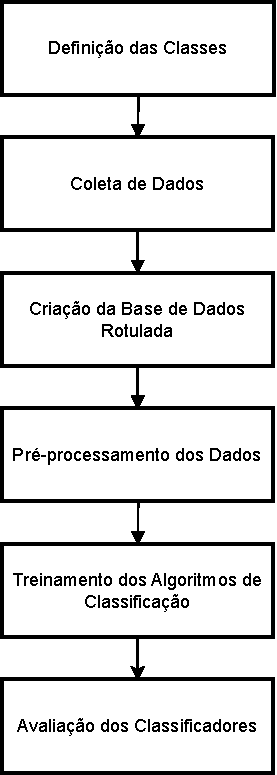
\includegraphics[width=0.25\linewidth]{metodologia_de_desenvolvimento2.pdf}
	\caption{Etapas do desenvolvimento deste estudo, que consiste em um método para avaliação de classificadores treinados na base de dados do Mercado Livre.}
	\label{fig:etapas_desenvolvimento}
\end{figure}

\section{Definição das Classes}
\label{definicao_classes}
Antes de coletar os dados que compuseram a base de dados, foi necessário definir quais atributos seriam considerados como classes. No Mercado Livre\footnote{\url{https://www.mercadolivre.com.br/}}, os produtos estavam organizados hierarquicamente em categorias. Essas categorias, por sua vez, estavam organizadas em um formato de Árvore de Categorias, que podia ser acessado com requisições via API\footnote{\url{https://developers.mercadolivre.com.br/pt_br/categorias-e-atributos}} usando o comando da Figura \ref{fig:comando_category_tree}.

\begin{figure}[htb]
    \centering
    \color{black}
    \begin{minted}{bash}
    $ curl https://api.mercadolibre.com/sites/MLB/categories/all > f.gz
    \end{minted}
    \caption{Comando para fazer \textit{download} de um arquivo compactado que possui a Árvore de Categorias completa do Mercado Livre brasileiro.}
    \label{fig:comando_category_tree}
\end{figure}

O Mercado Livre brasileiro possuía 32 categorias principais, e cada uma das categorias principais era dividida em dezenas de categorias secundárias, que por sua vez também podiam possuir outras subcategorias. Por exemplo, um carregador de celular era um produto que se encontrava em Celulares e Telefones > Acessórios para Celulares > Carregadores e Acessórios > Carregadores, de acordo com a estrutura proposta pelo Mercado Livre.

Como a GoBots fornece serviços para lojistas que vendem produtos das 11 categorias principais dispostas na Tabela \ref{table:categorias escolhidas}, essas foram as categorias de produtos escolhidas para compor a base de dados.

\begin{center}
\begin{table}[ht]
\caption{Categorias escolhidas para serem representadas na base de dados}
\label{table:categorias escolhidas}
\centering
    \begin{tabular}{|c|c|} 
     \hline
     \multicolumn{2}{|c|}{Categoria} \\
     \hline
     Acessórios para Veículos & Construção \\ 
     \hline
     Beleza e Cuidado Pessoal & Eletrodomésticos \\
     \hline
     Calçados, Roupas e Bolsas & Eletrônicos, Áudio e Vídeo \\
     \hline
     Câmeras e Acessórios & Esportes e Fitness\\
     \hline
     Casa, Móveis e Decoração & Ferramentas \\
     \hline
     Celulares e Telefones & \\
     \hline
    \end{tabular}
\end{table}
\end{center}

Para definir quais atributos serão considerados como classes, foi feito o \textit{download} da Árvore de Categorias usando o comando da Figura \ref{fig:comando_category_tree}. Em seguida, foi desenvolvido um código em \textit{Python} para percorrer essa Árvore de Categorias. Foram tomadas como base as categorias principais escolhidas e especificadas na Tabela \ref{table:categorias escolhidas}, e, após sucessivas iterações, juntou-se em uma lista todas as subcategorias dessas categorias principais, mantendo-se apenas as subcategorias que não possuem divisões.

Com a lista de todas as subcategorias desejadas disponível, novas requisições para a API do Mercado Livre foram feitas. Dessa vez, usando por milhares de vezes o comando da Figura \ref{fig:comando_category_attributes}, que retorna todos os atributos de uma determinada categoria. Com o auxílio de códigos em \textit{Python}, foram feitas transformações nesses dados: uma nova lista foi feita, descrevendo junto a cada subcategoria todos os seus possíveis atributos.

\begin{figure}[htb]
    \centering
    \color{black}
    \begin{minted}{bash}
    $ curl https://api.mercadolibre.com/categories/<id_cat>/attributes
    \end{minted}
    \caption{Comando para fazer \textit{download} de todos os atributos de uma determinada subcategoria do Mercado Livre brasileiro. \texttt{\textless id\_cat\textgreater} é um código único que identifica a subcategoria no conjunto de todas as categorias.}
    \label{fig:comando_category_attributes}
\end{figure}

Em seguida, foi criada uma nova lista com todos os atributos das subcategorias desejadas e o número de ocorrências em que esses atributos estão descritos nessas subcategorias. A Figura \ref{fig:top10_attributes} mostra os 10 atributos que mais aparecem nesse conjunto.

\begin{figure}[htb]
    \begin{lstlisting}[language=json,firstnumber=1]
    {
      "BRAND": 4892,
      "MODEL": 4892,
      "PACKAGE_HEIGHT": 4892,
      "PACKAGE_WIDTH": 4892,
      "PACKAGE_LENGTH": 4892,
      "PACKAGE_WEIGHT": 4892,
      "ITEM_CONDITION": 4892,
      "GTIN": 4890,
      "MPN": 4890,
      "SELLER_SKU": 4890,
      ...
    }
    \end{lstlisting}
    \caption{Os 10 atributos que são mais aceitos entre as subcategorias sem descendentes das categorias escolhidas e o número de subcategorias em que cada um aparece.}
    \label{fig:top10_attributes}
\end{figure}

Por último, foram escolhidos os atributos de maior interesse comercial da lista da Figura \ref{fig:top10_attributes} para serem as classes. O critério principal para a escolha foi selecionar aqueles atributos que descrevem o maior número de subcategorias diferentes. Após essa primeira etapa de escolha, foram feitos alguns refinamentos de forma manual para atingir o objetivo:

\begin{itemize}
  \item Remover atributos que raramente são questionados pelos clientes, tais como PACKAGE\_HEIGHT (altura do pacote);
  \item Remover atributos internos de uso privado do lojista e do Mercado Livre, tais como GTIN (código identificador de produtos interno do Mercado Livre);
  \item Dar preferência a atributos frequentemente perguntados pelos clientes;
  \item Dar preferência a atributos genéricos, ou seja, que se aplicam a uma grande variedade de produtos de diferentes categorias.
\end{itemize}

Ao todo, foram selecionados 39 atributos para serem as classes do problema, descritos pela Tabela \ref{table:atributos escolhidos}. Uma classe especial composta de exemplos que não pertencem à nenhuma das outras classes, a \textit{out\_of\_scope}, também foi escolhida. Portanto, a base de dados será composta por 40 classes.

\begin{table}[ht]
\caption{Classes escolhidas para serem representadas na base de dados}
\label{table:atributos escolhidos}
\tiny % Define o tamanho da fonte para small (opcional)
\begin{tabularx}{\textwidth}{|X|X|X|} 
 \hline
 \multicolumn{3}{|c|}{Classe} \\
 \hline
 BRAND & HEIGHT & SIZE \\ 
 \hline
 DETAILED\_MODEL & ALPHANUMERIC\_MODEL & MODEL \\
 \hline
 LINE & DIAMETER & ACCESSORIES\_INCLUDED \\
 \hline
 COMPATIBLE\_BRANDS & IS\_KIT & UNITS\_PER\_PACKAGE \\
 \hline
 DEPTH & MAIN\_MATERIAL & SHAPE \\
 \hline
 COLOR & ORIGIN & FABRIC\_DESIGN \\
 \hline
 THICKNESS & SALE\_FORMAT & WIDTH \\
 \hline
 RELEASE\_YEAR & POWER & MATERIALS \\
 \hline
 MAX\_WEIGHT\_SUPPORTED & LENGTH & WEIGHT \\
 \hline
 COMPOSITION & WAIST\_CIRCUMFERENCE & CHEST\_CIRCUMFERENCE \\
 \hline
 PART\_NUMBER & QUANTITY & PATTERN\_NAME \\
 \hline
 VOLUME\_CAPACITY & COMPATIBLE\_MODELS & MATERIAL \\
 \hline
 VOLTAGE & TOTAL\_LENGTH & HIP\_CIRCUMFERENCE \\
 \hline
 out\_of\_scope & & \\
 \hline
\end{tabularx}
\end{table}

% Árvore de categorias do Mercado Livre (API, esse posso mostrar com prints e com a URL da requisição)

% Selecionar quais categorias faziam mais sentido

% Definição de quais atributos (classes) seriam trabalhados: atributos genéricos e de utilidade no contexto de responder perguntas de clientes finais. Seleção dos atributos que se aplicam pro máximo de categorias possível! (não por número de produtos, e sim por número de categorias finais)

\section{Coleta de Dados}
\label{coleta_dados}

Como os modelos a serem treinados são modelos de Aprendizado Supervisionado, faz-se necessária a criação de uma base de dados rotulada. Neste trabalho, as etapas de Coleta de Dados e de Criação da Base Rotulada foram feitas de forma intercalada, isto é, enquanto não se atingiu um limiar mínimo de 15 exemplos para cada classe não foi finalizada a etapa de Coleta de Dados.

É importante esclarecer que todas as perguntas foram coletadas de acordo com a Lei Geral de Proteção de Dados Pessoais (LGPD) \cite{lgpd}. Dessa forma, as perguntas coletadas são dados impessoais, isto é, não contém informações sobre pessoas identificáveis, e portanto não permitem a identificação do autor ou de funcionários que trabalham no atendimento das lojas.

As perguntas foram coletadas de três diferentes fontes:

\begin{itemize}
  \item Em sua maioria, a partir do banco de dados da GoBots.
  
  Como a empresa fornece o serviço de resolução de dúvidas de clientes sobre produtos em plataformas de \textit{e-commerce} há alguns anos, muitos exemplos de perguntas feitas por clientes reais estão armazenados no banco de dados interno da empresa, do tipo \textit{MongoDB}\footnote{\url{https://www.mongodb.com/pt-br}}. Essas perguntas foram consideradas na criação da base de dados usada neste trabalho por serem perguntas de clientes reais. Por isso, espera-se que a qualidade da base de dados (e consequentemente, dos modelos treinados fazendo uso dela) aumente. Usando o \textit{MongoDB}, foi feita a exportação desses dados para um arquivo CSV.

  As perguntas coletadas por meio dessa fonte são dados de empresas que contrataram o serviço de automação da GoBots. Portanto, as empresas consentiram a coleta dessas perguntas para processamento posterior, o que inclui o processamento realizado neste trabalho. Uma parcela dessas perguntas pode ter sido feita em outros sites de \textit{e-commerce} além do Mercado Livre e incorporada ao banco de dados da GoBots em processamentos de dados anteriores.
  
  \item A partir de perguntas de clientes no Mercado Livre que estavam disponíveis de forma pública, mas que não faziam parte do banco de dados da GoBots.

  Algumas das classes selecionadas, como a COMPOSITION, são usadas apenas como atributos de categorias como Vestuário, que são constituídas de produtos que não são vendidos por clientes da GoBots. Por esse motivo, não existem exemplos dessas classes no banco de dados da GoBots. Para contornar esse problema, foi preciso pesquisar por produtos de Vestuário e outras categorias subrepresentadas no próprio site do Mercado Livre, e coletar perguntas reais que poderiam servir de exemplos para a criação da base de dados deste trabalho de forma manual.

  As perguntas coletadas por meio dessa fonte também foram coletadas como dados impessoais e seguindo os Termos e Condições do Programa de Desenvolvedores do Mercado Livre\footnote{\url{https://developers.mercadolivre.com.br/pt_br/termos-e-condicoes}}.
  
  \item A partir de criação manual, feita pelo próprio autor deste trabalho.

  A criação manual possui vieses pessoais, pois não representa as variadas formas de se perguntar que clientes reais podem criar, e isso pode afetar negativamente a qualidade da base de dados. No entanto, foi uma medida necessária para garantir que todas as 40 classes atingissem o limiar mínimo de 15 exemplos.
\end{itemize}

\section{Criação da Base de Dados Rotulada}
\label{criacao_base_dados_rotulada}
A Criação da Base de Dados Rotulada foi feita individualmente pelo autor deste trabalho. As perguntas que vieram do banco de dados da GoBots foram rotuladas por meio da execução de um \textit{script Python} disposto em um \textit{notebook Jupyter}\footnote{\url{https://jupyter.org}} hospedado na plataforma \textit{Google Colaboratory}\footnote{\url{https://colab.google}}. Os \textit{notebooks Jupyter} são uma forma interativa de executar programas escritos em \textit{Python}. Com eles, é possível executar trechos específicos de um programa ao invés do programa inteiro. O \textit{Google Colaboratory} é uma plataforma que fornece acesso gratuito à computação em nuvem e possui fácil integração com o servidor de hospedagem de arquivos \textit{Google Drive}\footnote{\url{https://drive.google.com}}, onde ficou armazenado o arquivo da base de dados.

O \textit{script} funciona da forma representada no Algoritmo \ref{algoritmo_1}.

% Define a style for Python code
\lstdefinestyle{python}{
    language=Python,
    basicstyle=\color{purple}\ttfamily, % Set the basic text color to purple
    keywordstyle=\color{blue},
    commentstyle=\color{green},
    stringstyle=\color{purple},
    numbers=left,
    numberstyle=\tiny\color{gray},
    frame=single,
    rulecolor=\color{black}, % Set the frame color to black
    breaklines=true,
    showstringspaces=false,
    escapechar=|
}

\begin{algorithm}[H]
\SetAlgoLined
\DontPrintSemicolon
\KwData{Arquivo CSV `dados.csv'}
\KwResult{Base de dados rotulada em JSON}
\BlankLine
Abra o arquivo CSV `dados.csv'\;
Conte o número de linhas no arquivo CSV e armazene em \textit{total\_linhas}\;
Gere um número aleatório, \textit{num\_aleatorio}, entre 0 e \textit{total\_linhas} - 1\;
\BlankLine
\While{True}{
  Leia a linha no índice \textit{num\_aleatorio} do arquivo CSV\;
  Escreva ``Exemplo a ser anotado: '' e o conteúdo da linha selecionada\;
  Leia ``Escolha um número entre 0 e 39 para classificar a sentença: ''\;
  \eIf{classe\_escolhida está entre 0 e 39}{
    Adicione a linha \{``exemplo'': linha selecionada, ``classe'': classe\_escolhida\} ao objeto JSON\;
    Salve o objeto JSON em `dados\_rotulados.json'\;
  }{
    Escreva ``Classe inválida''\;
  }
}
\KwRet\;
\caption{Seleção e Rotulação de Exemplos}
\label{algoritmo_1}
\end{algorithm}

A geração de um número aleatório se faz importante porque os dados do arquivo CSV foram coletados em ordem cronológica, do mais antigo ao mais novo. Por isso, houve a intenção de proporcionar uma maior variabilidade nos dados que poderiam ser rotulados a partir dessa fonte.

O terceiro, o quarto, o quinto e o sexto passos foram repetidos indefinidamente até que foi observado um acúmulo de exemplos de classes como BRAND e COLOR. Ao mesmo tempo, percebeu-se que classes como COMPOSITION e HIP\_CIRCUMFERENCE estavam subrepresentadas com menos de 15 exemplos. Neste instante, a rotulação de exemplos a partir do banco de dados da GoBots foi finalizada, e prosseguiu-se com a rotulação de exemplos a partir dos dados coletados via coleta manual no Mercado Livre e a partir dos dados coletados via criação manual.

Com a intenção de realizar uma segunda rodada de experimentos, na qual o desempenho dos modelos classificadores quando classes semelhantes são agrupadas é avaliado, foi feita uma aglutinação de classes. A aglutinação de classes foi pensada como um procedimento para diminuir o número de situações em que mais de uma classe poderia ser atribuída corretamente à mesma pergunta. Os modelos treinados não são capazes de classificar uma pergunta em mais de uma classe ao mesmo tempo, o que prejudica as métricas de avaliação.

Uma situação em que uma pergunta poderia ser classificada em mais de uma classe é quando, por exemplo, é feita a pergunta ``Este é o valor do par ou da unidade?''. Essa pergunta poderia ser classificada tanto como \textbf{\textit{UNITS\_PER\_PACKAGE}} quanto como \textbf{\textit{SALE\_FORMAT}}. A classe correta só poderia ser descoberta através de informações extras que os modelos não possuem acesso, como a subcategoria daquele produto em questão.

A Figura \ref{fig:aglutinacao_classes} retrata as aglutinações de classes que foram feitas. O novo arranjo propiciou que perguntas parecidas fizessem parte da mesma classe.

\begin{figure}[!htb]
        \centering
        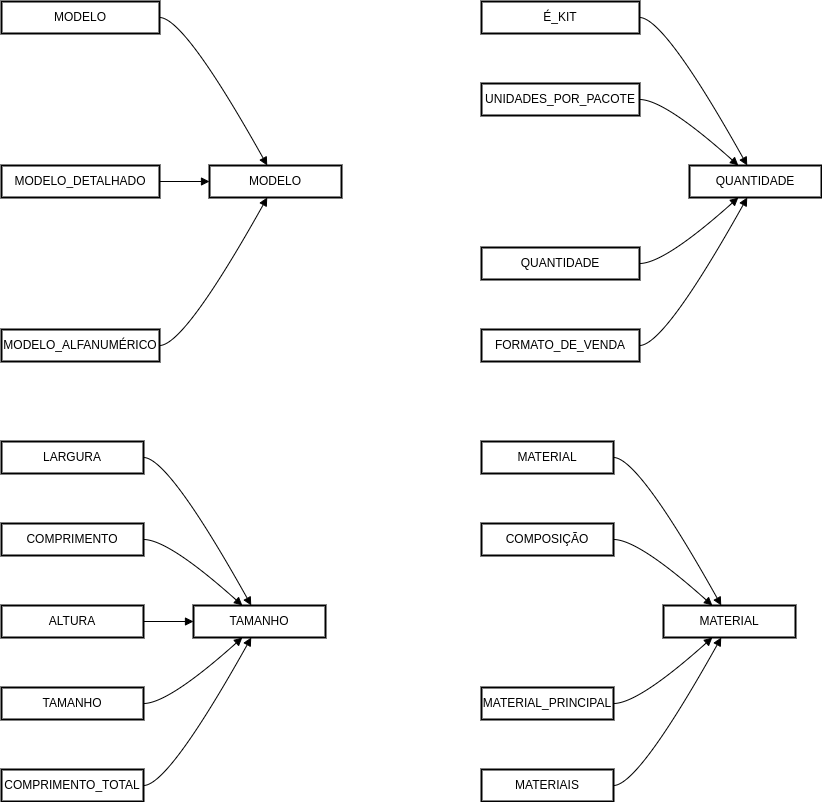
\includegraphics[width=14cm]{figuras/aglutinacao_de_classes_pt.png}
        \caption{Ao início de cada seta, as classes originais que compunham a base de dados com 40 classes. Ao final de cada seta, as classes resultantes da aglutinação, que passaram a compor a base de dados com 28 classes.}
        \label{fig:aglutinacao_classes}
\end{figure}

% Anotação (rotulagem) manual, iterando pelos exemplos das bases de dados da GoBots e assinalando um atributo para cada pergunta que aparecia

\section{Pré-processamento dos Dados}
\label{pre_processamento_dados}
A etapa de pré-processamento dos dados foi feita de forma diferente a depender da arquitetura de Transformador utilizada. Para a arquitetura que usa o modelo BERT para fazer a classificação, essa etapa foi feita apenas com o Tokenizador do modelo BERTimbau Base\footnote{\url{https://huggingface.co/neuralmind/bert-base-portuguese-cased}}, uma variação do modelo BERT pré-treinada em um grande corpus de dados da Internet escritos em Português do Brasil. Para a arquitetura que usa o modelo DIETClassifier para fazer a classificação, essa etapa foi feita com o Tokenizador do modelo BERTimbau Base ou com o Tokenizador do modelo BERT Multilingual Base\footnote{\url{https://huggingface.co/bert-base-multilingual-cased}}, e também com outros componentes extras, explicados na Subseção \ref{prepro_diet_classifier}. O BERT Multilingual Base é uma versão do BERT original desenvolvida pela \textit{Google} que apresenta suporte a 104 idiomas, incluindo o Português.

As etapas de pré-processamento citadas nesta Seção foram realizadas a partir da execução dos mesmos \textit{scripts} usados para o treinamento dos Algoritmos de Classificação: para a arquitetura que usa o modelo BERT para fazer a classificação, o \textit{script} escrito em \textit{Python} que chama funções da biblioteca \textit{HuggingFace Transformers}\footnote{\url{https://github.com/huggingface/transformers/}}; para a arquitetura que usa o modelo DIETClassifier para fazer a classificação, o \textit{script} de linha de comando \textit{rasa train}, incluso com o \textit{software} RASA\footnote{\url{https://rasa.com/}}.

Os exemplos coletados a partir da base de dados da GoBots já estavam sem sinais de pontuação, uma vez que essa etapa de pré-processamento já foi feita quando esses exemplos foram tratados pelo \textit{software} da empresa.

\subsection{BERT}
\label{prepro_bert}
O Tokenizador do modelo BERTimbau Base funciona dividindo a sentença fornecida como entrada em elementos de um vetor, dividindo palavras específicas em múltiplos \textit{tokens} (\textit{Stemming}), associando um número de identificação único a cada \textit{token}, e acrescentando \textit{tokens} especiais que indicam o início e o fim da sentença. Esse Tokenizador não aplica muitos dos passos da etapa de pré-processamento de dados vistos na Seção \ref{pre-processamento dos dados}, pois possui as seguintes caracerísticas:
\begin{itemize}
    \item \textit{Case sensitivity}: ``esse'' e ``Esse'' são tratados como \textit{tokens} diferentes, por exemplo, o que indica a não aplicação de \textit{lowercasing};
    \item Manutenção de \textit{stopwords}: palavras como ``os'' e ``de'' são consideradas \textit{tokens} válidos, por exemplo;
    \item Manutenção da pontuação e/ou números: o ponto de interrogação, por exemplo, é tratado como um \textit{token} individual;
    \item Não aplicação de \textit{Lemmatization}: ``bom'' e ``melhor'' são \textit{tokens} diferentes, por exemplo.
\end{itemize}

As Figuras \ref{fig:br_tokenizer_code} e \ref{fig:br_tokenizer_output} retratam como funciona o processo de Tokenização a partir do Tokenizador do modelo BERTimbau Base relatado. Na Figura \ref{fig:br_tokenizer_code}, \textit{tokenizer} é o Tokenizador do modelo BERTimbau Base, que foi baixado em linhas de código anteriores. Ao receber uma sentença como entrada, ele retorna um dicionário com as chaves ``input\_ids'', ``token\_type\_ids'' e ``attention\_mask'' (Figura \ref{fig:br_tokenizer_output}). O valor da chave ``input\_ids'' é uma lista de números de identificação únicos, onde cada número representa um \textit{token} e está mapeado internamente à uma representação vetorial daquele \textit{token}. Esse dicionário é o que é efetivamente fornecido como entrada ao algoritmo de classificação em treinamento. Se a função \textit{convert\_ids\_to\_tokens()} é chamada, é possível ver quais \textit{tokens} a lista de números de identificação únicos da chave ``input\_ids'' representa (Figura \ref{fig:br_tokenizer_output}).

\begin{figure}[!ht]
    \centering
    \begin{lstlisting}[style=python]
    encoded_text = tokenizer("Esse item |é| feito de silicone?")
    tokens = tokenizer.convert_ids_to_tokens(encoded_text["input_ids"])

    print(encoded_text)
    print(tokens)
    \end{lstlisting}
    \caption{Código em \textit{Python} que faz uso da biblioteca \textit{HuggingFace Transformers} para aplicar um Tokenizador do modelo BERTimbau Base à uma pergunta de um cliente real.}
    \label{fig:br_tokenizer_code}
\end{figure}

\begin{figure}[!ht]
    \centering
    \begin{verbatim}
    {'input_ids': [101, 3758, 18685, 253, 2160, 125, 7296, 10132, 
    22279, 136, 102], 'token_type_ids': [0, 0, 0, 0, 0, 0, 0, 0, 
    0, 0, 0], 'attention_mask': [1, 1, 1, 1, 1, 1, 1, 1, 1, 1, 1]}
    
    ['[CLS]', 'Esse', 'item', 'é', 'feito', 'de', 'sil', '##icon', 
    '##e', '?', '[SEP]']
    \end{verbatim}
    \caption{Saída do código \textit{Python} da Figura \ref{fig:br_tokenizer_code}, mostrando como a pergunta de um cliente real foi pré-processada pelo Tokenizador do modelo BERTimbau Base.}
    \label{fig:br_tokenizer_output}
\end{figure}

\subsection{DIETClassifier}
\label{prepro_diet_classifier}
Como descrito anteriormente, o uso de componentes extras em conjunto com a arquitetura de Transformador \textit{DIETClassifier} diferencia a sua etapa de pré-processamento dos dados em comparação com a etapa de pré-processamento dos dados usada com o BERT. Os componentes extras estão enunciados a seguir, ordenados do primeiro a ser usado ao último:

\begin{itemize}
    \item uma camada de \textit{WhitespaceTokenizer};
    
    O \textit{WhitespaceTokenizer} é um Tokenizador que separa as palavras nos espaços em branco. Além disso, sinais de pontuação no início ou no fim de palavras são removidos. Acentos são mantidos. 
    
    A Figura \ref{fig:whitespace_tokenizer} retrata como o Tokenizador \textit{WhitespaceTokenizer} funciona. Uma lista de \textit{tokens} foi gerada, e cada \textit{token} representa uma palavra da sentença ``Esse item é feito de silicone?''. O acento agudo em ``é'' foi mantido, mas o ponto de interrogação ao final da sentença foi removido, pois ele está ao final de uma palavra. Um \textit{token} especial, chamado de ``\_\_CLS\_\_'', foi introduzido para indicar o fim da sentença.
    
    \item uma camada de \textit{LanguageModelFeaturizer} (constituída pelo Tokenizador do modelo BERTimbau Base ou pelo Tokenizador do modelo BERT Multilingual Base, a depender do experimento);

    O \textit{LanguageModelFeaturizer} funciona da mesma forma que o Tokenizador descrito na Subseção \ref{prepro_bert}.
    
    \item duas camadas de \textit{CountVectorsFeaturizer}.

    O \textit{CountVectorsFeaturizer} é um componente responsável pela transformação dos \textit{tokens} em representações vetoriais. Ele cria representações vetoriais no formato \textit{bag-of-words} da entrada recebida. Na arquitetura de Transformador que usa o modelo DIETClassifier para fazer a classificação, o componente \textit{CountVectorsFeaturizer} foi usado duas vezes: na primeira vez, representações \textit{bag-of-words} foram feitas a nível de palavras; na segunda vez, representações \textit{bag-of-words} foram feitas a nível de sequências de 1 a 5 caracteres. 
    
    A Figura \ref{fig:rasa_tokenizers} retrata como o \textit{CountVectorsFeaturizer} funciona quando aplicado após uma camada de \textit{WhitespaceTokenizer} e uma camada de \textit{LanguageModelFeaturizer}. 
    
    Na parte central da Figura \ref{fig:rasa_tokenizers}, são mostrados os vetores gerados após a aplicação da primeira camada de \textit{CountVectorsFeaturizer}, sendo o primeiro vetor um vetor de \textit{tokens} e o segundo vetor um vetor que indica a quantidade de vezes que cada \textit{token} aconteceu em cada sentença. Os vetores gerados apresentam grande diferença em relação à lista de \textit{tokens} da Figura \ref{fig:whitespace_tokenizer}. Todos os \textit{tokens} ficaram com letras minúsculas. A palavra ``silicone'' foi dividida em múltiplos \textit{tokens}, por causa do \textit{LanguageModelFeaturizer}. `cls' e `sep' são os \textit{tokens} especiais ``\_\_CLS\_\_'' e ``\_\_SEP\_\_'', usados para indicar o fim de cada sentença e o início de uma sentença nova, respectivamente.

    Na parte inferior da Figura \ref{fig:rasa_tokenizers}, são mostrados os vetores gerados após a aplicação da segunda camada de \textit{CountVectorsFeaturizer}. Os \textit{tokens} apresentados são constituídos de todas as sequências de 5 caracteres possíveis de serem criadas a partir das sentenças fornecidas como entrada. Os símbolos \# representam os \textit{tokens} criados a partir da divisão de uma palavra em múltiplos \textit{tokens} (``silicone'' se tornou ``sil'', ``\#\#icon'', ``\#\#e''). Todos os \textit{tokens} ficaram com letras minúsculas. `[cls]' e `[sep]' são os mesmos \textit{tokens} especiais explicados anteriormente. Os vetores constituídos de 1 e 0 na parte inferior indicam quantas vezes cada sequência de 5 caracteres acontece em cada sentença fornecida como entrada.
    
\end{itemize}

\begin{figure}[!ht]
    \begin{subfigure}{\linewidth}
        \centering
        \begin{lstlisting}[style=python]
        "Esse item |é| feito de silicone?"
        \end{lstlisting}
    \end{subfigure}
    
    \begin{subfigure}{\linewidth}
        \centering
        \begin{verbatim}
        ['Esse', 'item', 'é', 'feito', 'de', 'silicone', '__CLS__']
        \end{verbatim}
    \end{subfigure}
    
    \caption{Exemplo de aplicação do Tokenizador \textit{WhitespaceTokenizer}.}
    \label{fig:whitespace_tokenizer}
\end{figure}

\begin{figure}[!ht]
    \begin{subfigure}{\linewidth}
        \centering
        \begin{lstlisting}[style=python]
        ["Esse item |é| feito de silicone?", 
         "Esse item |é| feito de pl|á|stico?"]
        \end{lstlisting}
        \caption{Sentenças de exemplo fornecidas como entrada aos tokenizadores.}
    \end{subfigure}
    
    \hrulefill
    \\
    
    \begin{subfigure}{\linewidth}
        \centering
        \begin{verbatim}
        ['cls' 'de' 'esse' 'feito' 'icon' 'item' 'plástico' 'sep' 'sil']
        [[1 1 1 1 1 1 0 1 1]
        [1 1 1 1 0 1 1 1 0]]
        \end{verbatim}
        \caption{Representações \textit{bag-of-words} a nível de palavras geradas a partir da aplicação dos tokenizadores sobre as sentenças de exemplo fornecidas como entrada.}
    \end{subfigure}

    \hrulefill
    \\

    \begin{subfigure}{\linewidth}
        \centering
        \begin{verbatim}
        ['##e[s' '##ico' '#e[se' '#icon' '[cls]' '[sep]' ']esse' 'cls]e' 
         'co[se' 'con##' 'deplá' 'desil' 'e[sep' 'eitem' 'eitod' 'eméfe' 
         'eplás' 'esil#' 'essei' 'feito' 'ico[s' 'icon#' 'il##i' 'itemé' 
         'itode' 'l##ic' 'ls]es' 'lásti' 'méfei' 'n##e[' 'o[sep' 'odepl' 
         'odesi' 'on##e' 'plást' 's]ess' 'seite' 'sil##' 'sseit' 'stico' 
         'teméf' 'tico[' 'todep' 'todes' 'ástic' 'éfeit']
        [[1 1 1 1 1 1 1 1 0 1 0 1 1 1 1 1 0 1 1 1 0 1 1 1 1 1 1 0 1 1 0
        0 1 1 0 1 1 1 1 0 1 0 0 1 0 1]
        [0 0 0 0 1 1 1 1 1 0 1 0 0 1 1 1 1 0 1 1 1 0 0 1 1 0 1 1 1 0 1
        1 0 0 1 1 1 0 1 1 1 1 1 0 1 1]]
        \end{verbatim}
        \caption{Representações \textit{bag-of-words} a nível de sequências de 5 caracteres geradas a partir da aplicação dos tokenizadores sobre as sentenças de exemplo fornecidas como entrada.}
    \end{subfigure}

    \caption{Resultado após aplicação dos Tokenizadores \textit{WhitespaceTokenizer}, \textit{LanguageModelFeaturizer} e duas camadas de \textit{CountVectorsFeaturizer} em sequência sobre duas sentenças de exemplo.}
    \label{fig:rasa_tokenizers}
\end{figure}

\section{Treinamento dos Algoritmos de Classificação}
\label{algoritmos_classificacao}
Esta seção descreve o método de treinamento dos dois Algoritmos de Classificação usados: BERT e DIETClassifier. Ambos os Algoritmos de Classificação foram treinados por meio de \textit{fine-tuning}, conceito explicado na Subseção \ref{bert_subsubsection}.

As seções de treinamento foram feitas através da plataforma \textit{Google Colaboratory}, em virtude da disponibilidade gratuita de placas de vídeo dedicadas de alto poder computacional. O acesso a esse recurso tornou possível que cada treinamento levasse no máximo 2 horas de duração.

\subsection{BERT}
\label{des_treinamento_hf}
Ao invés de usar o Transformador BERT original, apresentado em \citeonline{bert}, optou-se por usar o BERTimbau Base, apresentado em \citeonline{bertimbau}. Essa escolha foi feita com base nos resultados de experimentos anteriores de outros projetos da empresa GoBots, nos quais chegou-se à conclusão de que modelos treinados com \textit{tokens} em Português apresentam melhores resultados para aplicações em Português, como é o caso deste trabalho.

Os modelos BERTimbau são definidos pelos seus criadores como ``modelos BERT para Português Brasileiro, treinados usando dados do brWaC, um grande \textit{corpus} de páginas Web'' \cite{bertimbau}. À época, os modelos BERTimbau avançaram o estado-da-arte das abordagens BERT multilíngua e monolíngua. O termo Base se refere ao tamanho do modelo menor, de 12 camadas e 110 milhões de parâmetros. Ambos os modelos foram disponibilizados pelos autores para \textit{download} gratuito em bibliotecas \textit{open-source}.

Todas as etapas que usaram o Algoritmo de Classificação BERTimbau Base, do pré-processamento dos dados à Avaliação dos Classificadores, foram feitas por meio de chamadas às funções da biblioteca \textit{HuggingFace Transformers}, escrita na linguagem \textit{Python}. Por meio dela, é possível definir os hiperparâmetros de treino e efetivamente treinar o Algoritmo de Classificação. Para isso, basta que a base de dados esteja em um formato compatível, como JSON ou CSV.

A biblioteca \textit{HuggingFace Transformers} permite a alteração dos hiperparâmetros de treino, tais como \textit{batch\_size} (a quantidade de exemplos vistos a cada passo de treinamento) e \textit{learning\_rate} (o fator pelo qual os pesos do Algoritmo de Classificação em treinamento são multiplicados durante o processo). Por isso, o BERTimbau Base foi treinado em 2 configurações: 

\begin{itemize}
    \item na primeira, identificada como HF1, com quantidade de exemplos a cada passo = 8 exemplos.
    \item na segunda, identificada como HF2, com quantidade de exemplos a cada passo = 1 exemplo. 
\end{itemize}

Ao alterar o número de exemplos que o Algoritmo de Classificação em treinamento vê a cada passo, aumenta-se o número de passos totais para que ele veja todos os exemplos. Assim, ao ver menos exemplos por vez, o Algoritmo é otimizado mais vezes. Foram feitos 5 treinamentos em cada configuração para buscar validade estatística (ou seja, para desprezar efeitos do acaso nas medidas de avaliação que aquele Algoritmo de Classificação atingiu).

Duas rodadas de experimentos foram feitas com o BERTimbau Base: na primeira, as duas configurações HF1 e HF2 foram treinadas na base de dados rotulada em 40 classes. Na segunda rodada de experimentos, foi escolhida a configuração com o melhor desempenho nas medidas de avaliação da primeira rodada para ser treinada na base de dados rotulada em 28 classes.

\subsection{DIETClassifier}
\label{des_treinamento_rasa}
O outro algoritmo de classificação que foi treinado foi o Transformador DIETClassifier, apresentado em \citeonline{diet_classifier}. Um dos motivos pelo qual ele foi escolhido é por causa da modularidade da sua arquitetura, que permite que sejam usados Tokenizadores de variados métodos de pré-treino, assim como outros componentes, em conjunto com ele. Outro motivo para a escolha é que os autores alegam que o melhor modelo DIETClassifier supera um modelo BERT que passou por \textit{fine-tuning} e ainda é seis vezes mais rápido de se treinar \cite{diet_classifier}.

Todas as etapas que usaram o Algoritmo de Classificação DIETClassifier, do pré-processamento dos dados à Avaliação dos Classificadores, foram feitas por meio do \textit{software} de linha de comando RASA \textit{Open Source}. A instalação\footnote{\url{https://rasa.com/docs/rasa/installation/installing-rasa-open-source}} se dá pelo Gerenciador de Pacotes do \textit{Python}, o PIP. Depois disso, é preciso criar um projeto com o comando \textit{rasa init} e procurar os arquivos recém-criados \textit{data/nlu.yml} e \textit{config.yml}. No primeiro arquivo são inseridos todos os exemplos da base de dados. No segundo arquivo são inseridas as especificações de todos os componentes das etapas de pré-processamento dos dados e de Treinamento dos Algoritmos de Classificação. Após o preenchimento dos dois arquivos, é possível começar o treinamento do DIETClassifier com o comando \textit{rasa train nlu}.


O \textit{software} RASA \textit{Open Source} permite a adição e personalização dos componentes do Transformador que será treinado, tais como o \textit{FallbackClassifier}, que retorna uma classe especial indicando que não foi possível prever com assertividade a qual classe aquele exemplo pertence caso a pontuação \textit{confidence} não tenha atingido um valor mínimo de 0.7. Além disso, existe o parâmetro \textit{constrain\_similarities}, que pode ser aplicado ao Algoritmo de Classificação para que seja executada uma função extra para diminuir a similaridade entre a sentença fornecida como entrada e sentenças de outras classes. O DIETClassifier foi treinado em 3 configurações: 

\begin{itemize}
    \item na primeira, identificada como RASA1, o \textit{LanguageModelFeaturizer} usado foi o BERT Multilingual Base, o componente CountVectorsFeaturizer foi configurado para criar representações \textit{bag-of-words} de sequências de 1 a 4 caracteres, o parâmetro \textit{constrain\_similarities} foi definido como verdadeiro e o componente \textit{FallbackClassifier} foi utilizado;
    \item na segunda, identificada como RASA2, o \textit{LanguageModelFeaturizer} usado foi o BERTimbau Base, o componente CountVectorsFeaturizer foi configurado para criar representações \textit{bag-of-words} de sequências de 3 a 5 caracteres, o parâmetro \textit{constrain\_similarities} foi definido como falso e o componente \textit{FallbackClassifier} não foi utilizado;
    \item na terceira, identificada como RASA3, o \textit{LanguageModelFeaturizer} usado foi o BERTimbau Base, o componente CountVectorsFeaturizer foi configurado para criar representações \textit{bag-of-words} de sequências de 3 a 5 caracteres, o parâmetro \textit{constrain\_similarities} foi definido como verdadeiro e o componente \textit{FallbackClassifier} foi utilizado.
\end{itemize}

Duas rodadas de experimentos foram feitas com o DIETClassifier: na primeira, as três configurações RASA1, RASA2 e RASA3 foram treinadas na base de dados rotulada em 40 classes. Na segunda rodada de experimentos, foi escolhida a configuração com o melhor desempenho nas medidas de avaliação da primeira rodada para ser treinada na base de dados rotulada em 28 classes. Foram feitos
5 treinamentos em cada configuração para buscar validade estatística.

\section{Medidas e Método de Avaliação dos Classificadores}
\label{medidas_metodo_avaliacao_classificadores}
Os testes (e consequentemente, a geração de métricas) foram executados pela biblioteca \textit{HuggingFace Transformers} (no caso do BERTimbau Base) ou através de um comando do \textit{software RASA} (no caso do DIETClassifier). Na biblioteca \textit{HuggingFace Transformers}, basta que seja usado o parâmetro \textit{compute\_metrics=} e seja fornecida a função responsável por calcular as métricas. Além das métricas geradas ao final, a biblioteca \textit{HuggingFace Transformers} calcula métricas preliminares toda vez que todos os exemplos de Treinamento são vistos. Contudo, as métricas preliminares foram descartadas, pois não são importantes para os objetivos deste estudo.  No \textit{software RASA Open Source}, a geração de métricas é feita por padrão, sem a adição de novos parâmetros.

Não foi realizada Validação Cruzada nos experimentos com o BERTimbau como Algoritmo de Classificação. A estratégia empregada foi a separação dos dados de Treino e Teste. Os exemplos de Teste, que compõem 20\% da base de dados total, foram usados para os testes, e não influenciaram nos pesos do algoritmo de classificação em treinamento. Os exemplos de Treino, que compõem 80\% da base de dados total, foram usados para o treinamento. Os experimentos foram feitos desta forma por causa da alta demanda de recursos computacionais para realizar Validação Cruzada em treinamentos de modelos BERT, que aumentaria em 5 vezes o tempo necessário para cada um dos 5 treinamentos para ambas as configurações HF1 e HF2.  Além disso, a biblioteca \textit{HuggingFace Transformers} não apresenta suporte nativo a Validação Cruzada, o que dificulta a implementação.

Foi realizada Validação Cruzada nos experimentos com o DIETClassifier, pelo fato deste Algoritmo de Classificação não demandar tantos recursos computacionais para isso quanto o BERTimbau Base. A base de dados definida no arquivo \textit{data/nlu.yml} foi dividida em 5 partes: a cada treinamento, 4 partes eram definidas como exemplos de Treino, e 1 parte era definida como exemplos de Teste, em um processo iterativo. Após todas as partes terem sido definidas como exemplos de Teste, o Treinamento foi finalizado. As métricas de avaliação daquele Treinamento como um todo eram tomadas a partir da média das métricas de avaliação de cada etapa de Validação Cruzada.

É importante salientar que o uso de dois métodos diferentes de avaliação faz com que as métricas encontradas nos experimentos com o algoritmo de classificação BERTimbau não possam ser comparadas com as métricas encontradas nos experimentos com o algoritmo de classificação DIETClassifier. O principal motivo para não se realizar Validação Cruzada na avaliação dos modelos BERTimbau é o fato de que essa técnica aumenta em cinco vezes o número de treinamentos, o que faria que o tempo total gasto com treinamento e avaliação dos modelos BERTimbau passasse de 30 horas para 150 horas e prejudicaria a conclusão dos experimentos.

Além das métricas Acurácia, Precisão, Revocação e F1-Score, as Matrizes de Confusão, como são um bom recurso para comparar o desempenho dos modelos classe a classe e para enxergar pontos fortes e fracos, também foram geradas. A biblioteca \textit{HuggingFace Transformers} não cria Matrizes de Confusão por padrão. Por isso, quando treinando o Transformador que tem como Algoritmo de Classificação o BERTimbau Base, elas foram produzidas com chamadas aos elementos confusion\_matrix() e ConfusionMatrixDisplay() da biblioteca \textit{sklearn.metrics}\footnote{\url{https://scikit-learn.org/stable/modules/generated/sklearn.metrics.confusion_matrix.html}}. Essas chamadas foram adicionadas à função compute\_metrics(). No \textit{software RASA Open Source}, as Matrizes de Confusão são geradas sem adição de código extra.

As métricas F1, Precisão e Revocação foram ponderadas, ou seja, os valores das métricas dependeram também do número de exemplos daquela classe na base de dados. Essa escolha pela ponderação foi feita porque a base de dados é desbalanceada, com algumas classes tendo mais exemplos do que outras. A ponderação é feita fazendo um somatório da multiplicação entre uma métrica de uma classe pela razão entre o número de exemplos daquela classe e o número de exemplos total, como mostra a Equação \ref{eq_weighted}.

\begin{equation}
\label{eq_weighted}
\text{Métrica\_ponderada} = \sum \text{Métrica}_k \cdot \frac{\text{Quant\_exemplos}_k}{\text{Quant\_exemplos}_{\text{total}}}
\end{equation}

\section{Considerações Finais}
Para o desenvolvimento deste estudo, foram aplicadas diferentes abordagens de Classificação de Texto a um problema prático consistido em definir a qual atributo uma determinada pergunta de um usuário real do Mercado Livre se refere.

Na primeira etapa, 39 atributos importantes foram selecionados para serem as classes para as quais as arquiteturas de Transformadores seriam treinadas. Na segunda etapa, dados não-rotulados foram coletados de diferentes fontes. Na terceira etapa, esses dados foram rotulados com o objetivo de criar uma base de dados rotulada. Essa base de dados consiste de 1419 exemplos. Uma segunda rotulação de exemplos com 28 atributos foi feita para que fossem possíveis novos experimentos.

Em seguida, foram definidas formas diferentes de se realizar o pré-processamento dos dados. Para a arquitetura de Transformador que faz uso do classificador BERTimbau Base, apenas o Tokenizador desse classificador foi utilizado. No entanto, para a arquitetura de Transformador que faz uso do classificador DIETClassifier, outros componentes como o \textit{WhitespaceTokenizer} e o \textit{CountVectorsFeaturizer} também foram testados em conjunto com o Tokenizador do BERT Multilingual Base e o Tokenizador do BERTimbau Base.

Finalmente, foi feito o treinamento: 2 configurações diferentes de Transformadores com BERTimbau Base e 3 configurações diferentes de Transformadores com DIETClassifier foram treinadas, 5 vezes cada para que os resultados tenham validade estatística. As configurações com as melhores métricas passaram por uma nova rodada de experimentos sendo treinadas na base de dados com 28 classes. O cálculo de métricas como Acurácia, Precisão, Revocação e F1-Score, assim como a elaboração de Matrizes de Confusão, foi adicionado ao código que faz o treinamento para que fosse possível comparar os modelos treinados.

%TCC:
%TCC:
%TCC:
%TCC:



% ----------------------------------------------------------
% Resultados
% ----------------------------------------------------------
\chapter[Resultados]{Resultados}
\label{cap-resultados}
Este capítulo tem como objetivo descrever e analisar os resultados obtidos pelas etapas descritas no capítulo anterior, desde a definição das classes até as métricas e métodos de avaliação dos classificadores treinados.

A Seção \ref{res:definicao_classes} discorre sobre os atributos escolhidos para serem classes e os motivos para que sua escolha tenha sido feita.

A Seção \ref{res:coleta_dados} apresenta a representatividade de cada fonte de coleta de dados no conjunto de todos os exemplos rotulados, enquanto a Seção \ref{res:criacao_base_dados_rotulada} mostra a distribuição de exemplos em cada classe da base de dados rotulada, antes e depois da execução do procedimento de aglutinação de classes.

A Seção \ref{res:treinamento_avaliacao_dos_classificadores} mostra a divisão da base de dados em subconjuntos de Treino e Teste, apresenta os resultados da avaliação de todos os modelos, considerando tanto a base de dados com 40 classes quanto a base de dados com 28 classes, traça comparações entre os modelos e sumariza as classes em que os modelos apresentaram o melhor e o pior desempenho.

A Seção \ref{res:comparativo_entre_classes_confundidas} visa elucidar os motivos por trás do desempenho ruim de todos os modelos em uma classe específica.

\section{Definição das Classes}
\label{res:definicao_classes}
Como visto na Seção \ref{definicao_classes}, quatro critérios foram aplicados nos atributos que aparecem no maior número de subcategorias do Mercado Livre (mostrados na Figura \ref{fig:top10_attributes}) para definir os 39 atributos (ou classes) com maior interesse comercial.

A Figura \ref{fig:atributos_em_numero_de_subcategorias} mostra, por meio de uma Nuvem de Palavras, a representatividade dos 39 atributos de maior interesse comercial escolhidos em termos do número de subcategorias do Mercado Livre em que esses atributos podem ser usados. Percebe-se pela Figura \ref{fig:atributos_em_numero_de_subcategorias} e pela análise do JSON, extraído a partir das requisições à API do Mercado Livre, que \textbf{BRAND} e \textbf{MODEL} são os atributos mais genéricos que se encaixam nos critérios aplicados. Ambos os atributos podem ser usados em 4892 subcategorias de produtos.

\begin{figure}[!ht]
    \centering
	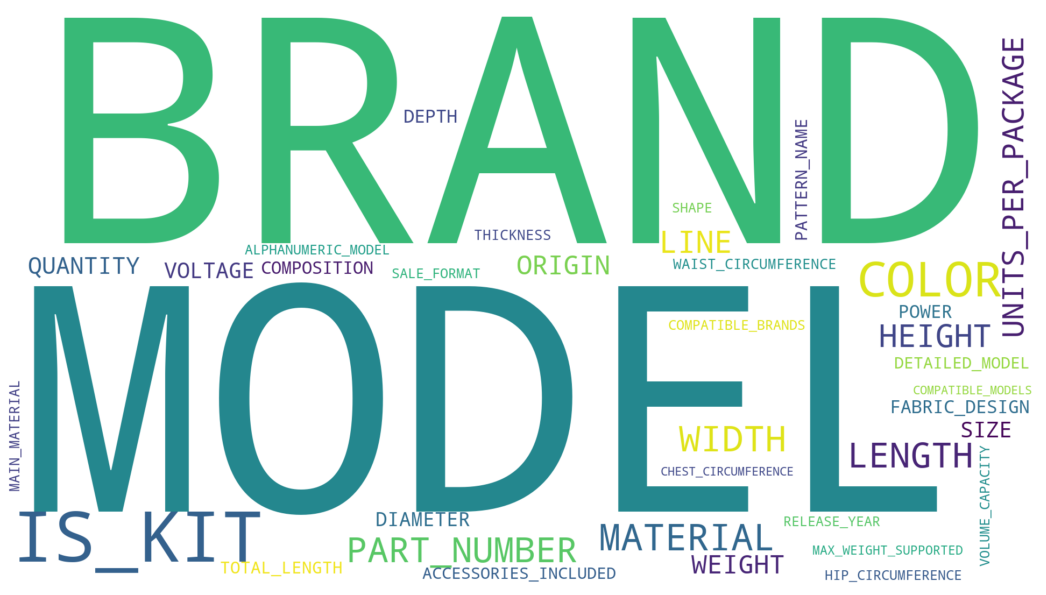
\includegraphics[width=0.80\linewidth]{atributos_em_numero_de_subcategorias.png}
	\caption{Nuvem de Palavras com os 39 atributos escolhidos para serem classes. O tamanho das palavras reflete o número de subcategorias do Mercado Livre em que esses atributos podem ser usados.}
	\label{fig:atributos_em_numero_de_subcategorias}
\end{figure}

Por outro lado, os atributos menos genéricos que foram definidos como classes, pois se encaixam nos critérios aplicados, são \textbf{CHEST\_CIRCUMFERENCE} e \textbf{COMPATIBLE\_MODELS}. Ambos os atributos podem ser usados em 87 subcategorias de produtos. \textbf{CHEST\_CIRCUMFERENCE}, traduzido como ``circunferência do busto'' em Português, se aplica apenas a itens de Vestuário, setor em que a empresa GoBots ainda não possui clientes, e por isso representa um bom experimento para avaliar a possibilidade de atração de clientes do setor. \textbf{COMPATIBLE\_MODELS}, de forma similar, é usado para descrever apenas a compatibilidade de peças e acessórios, como motores e válvulas, com modelos de objetos maiores, como veículos e eletrodomésticos. Portanto, o baixo número de subcategorias onde esses atributos podem ser usados se justifica pela especificidade de suas aplicações.

\section{Coleta de Dados}
\label{res:coleta_dados}
A Tabela \ref{table:coleta de dados} apresenta uma estimativa de qual porcentagem cada fonte de coleta de dados representa em relação a base de dados criada. A maior parte das perguntas, estimada em 70\%, foi coletada a partir do banco de dados da GoBots, que já existia anteriormente. Os outros 30\% foram coletados por meio de coleta manual no mercadolivre.com.br ou através de criação manual, em um esforço para garantir que cada classe possuísse pelo menos 15 exemplos. A coleta de dados através de criação manual foi de apenas 10\%, com o objetivo de fazer com que os exemplos vistos fossem, em sua grande maioria, representações da forma de perguntar de clientes reais. Em virtude do alto número de exemplos, não é possível saber com exatidão quantos exemplos foram coletados de cada fonte.

\begin{center}
\begin{table}[!ht]
\caption{Fontes para Coleta de Dados e estimativa de sua representatividade na base de dados}
\label{table:coleta de dados}
\centering
    \begin{tabular}{|c|c|} 
     \hline
     \multicolumn{2}{|c|}{Fonte dos Dados} \\
     \hline
     Banco de Dados da GoBots & 70\% \\ 
     \hline
     Coleta manual no mercadolivre.com.br & 20\% \\
     \hline
     Criação manual & 10\% \\
     \hline
     Total & 1419 \\
     \hline
    \end{tabular}
\end{table}
\end{center}

\section{Criação da Base de Dados Rotulada}
\label{res:criacao_base_dados_rotulada}
Como visto na Seção \ref{criacao_base_dados_rotulada}, a criação da base de dados rotulada ocorreu em duas rodadas. Na primeira rodada, as perguntas foram rotuladas em relação aos atributos a que elas se referem, considerando 40 atributos descritores de produtos do Mercado Livre. Na segunda rodada, atributos similares foram aglutinados em um único atributo, com o objetivo de minimizar a ocorrência de situações em que uma pergunta poderia ser classificada em mais de um atributo ao mesmo tempo. Isso proporcionou com que uma nova rotulação, baseada em 28 classes ao invés de 40, pudesse ser feita. 

A Tabela \ref{table:divisão_de_classes} apresenta a quantidade de exemplos rotulados para cada classe considerando a configuração inicialmente proposta na primeira rodada de experimentos, constituída de 40 classes:

\begin{table}[!htb]
\caption{Quantidade de exemplos rotulados para cada classe na configuração com 40 classes}
\label{table:divisão_de_classes}
\tiny % Define o tamanho da fonte para small (opcional)
\begin{tabularx}{\textwidth}{|X|c|X|c|}
 \hline
 \textbf{Classe} & \textbf{Exemplos} & \textbf{Classe} & \textbf{Exemplos} \\
 \hline
 BRAND & \textbf{105} & MODEL & \textbf{32} \\
 \hline
 IS\_KIT & \textbf{18} & COLOR & \textbf{94} \\
 \hline
 WIDTH & \textbf{32} & LENGTH & \textbf{29} \\
 \hline
 PART\_NUMBER & \textbf{21} & MATERIAL & \textbf{58} \\
 \hline
 HEIGHT & \textbf{41} & LINE & \textbf{23} \\
 \hline
 UNITS\_PER\_PACKAGE & \textbf{22} & ORIGIN & \textbf{25} \\
 \hline
 RELEASE\_YEAR & \textbf{27} & WEIGHT & \textbf{22} \\
 \hline
 QUANTITY & \textbf{23} & VOLTAGE & \textbf{60} \\
 \hline
 SIZE & \textbf{80} & DIAMETER & \textbf{26} \\
 \hline
 DEPTH & \textbf{21} & FABRIC\_DESIGN & \textbf{16} \\
 \hline
 POWER & \textbf{33} & COMPOSITION & \textbf{18} \\
 \hline
 PATTERN\_NAME & \textbf{16} & TOTAL\_LENGTH & \textbf{23} \\
 \hline
 DETAILED\_MODEL & \textbf{72} & ACCESSORIES\_INCLUDED & \textbf{55} \\
 \hline
 MAIN\_MATERIAL & \textbf{16} & THICKNESS & \textbf{29} \\
 \hline
 MATERIALS & \textbf{35} & WAIST\_CIRCUMFERENCE & \textbf{16} \\
 \hline
 VOLUME\_CAPACITY & \textbf{23} & HIP\_CIRCUMFERENCE & \textbf{15} \\
 \hline
 ALPHANUMERIC\_MODEL & \textbf{23} & COMPATIBLE\_BRANDS & \textbf{20} \\
 \hline
 SHAPE & \textbf{20} & SALE\_FORMAT & \textbf{34} \\
 \hline
 MAX\_WEIGHT\_SUPPORTED & \textbf{32} & CHEST\_CIRCUMFERENCE & \textbf{15} \\
 \hline
 COMPATIBLE\_MODELS & \textbf{48} & out\_of\_scope & \textbf{101} \\
 \hline
 \multicolumn{3}{|l|}{\textbf{Total de Exemplos}} & \textbf{1419} \\
 \hline
\end{tabularx}
\end{table}

É possível perceber o desbalanceamento entre o número de exemplos de cada classe. Esse desbalanceamento ocorreu, sobretudo, por conta da facilidade em se encontrar perguntas relacionadas a atributos como marca e cor do produto (perguntas classificadas como \textbf{BRAND} e \textbf{COLOR}) em detrimento da dificuldade de se encontrar perguntas relacionadas a atributos como a estampa de uma peça de roupa e os modelos compatíveis (perguntas classificadas como \textbf{FABRIC\_DESIGN} e \textbf{COMPATIBLE\_MODELS}). Essa dificuldade se justifica pelo menor número de subcategorias de produtos que podem receber esses atributos, como abordado na Seção \ref{res:definicao_classes}. A Figura \ref{fig:número_de_exemplos_40_classes} retrata, por meio de um gráfico de barras, o número de exemplos rotulados em cada classe.
% Gráfico de barras pras pessoas verem pelo tamanho das barras as classes com os maiores números de exemplos. É válido ter duas formas de representação gráfica pros mesmos dados.
% Gráfico de barras - 40 classes

\begin{figure}[!htb]
    \centering
	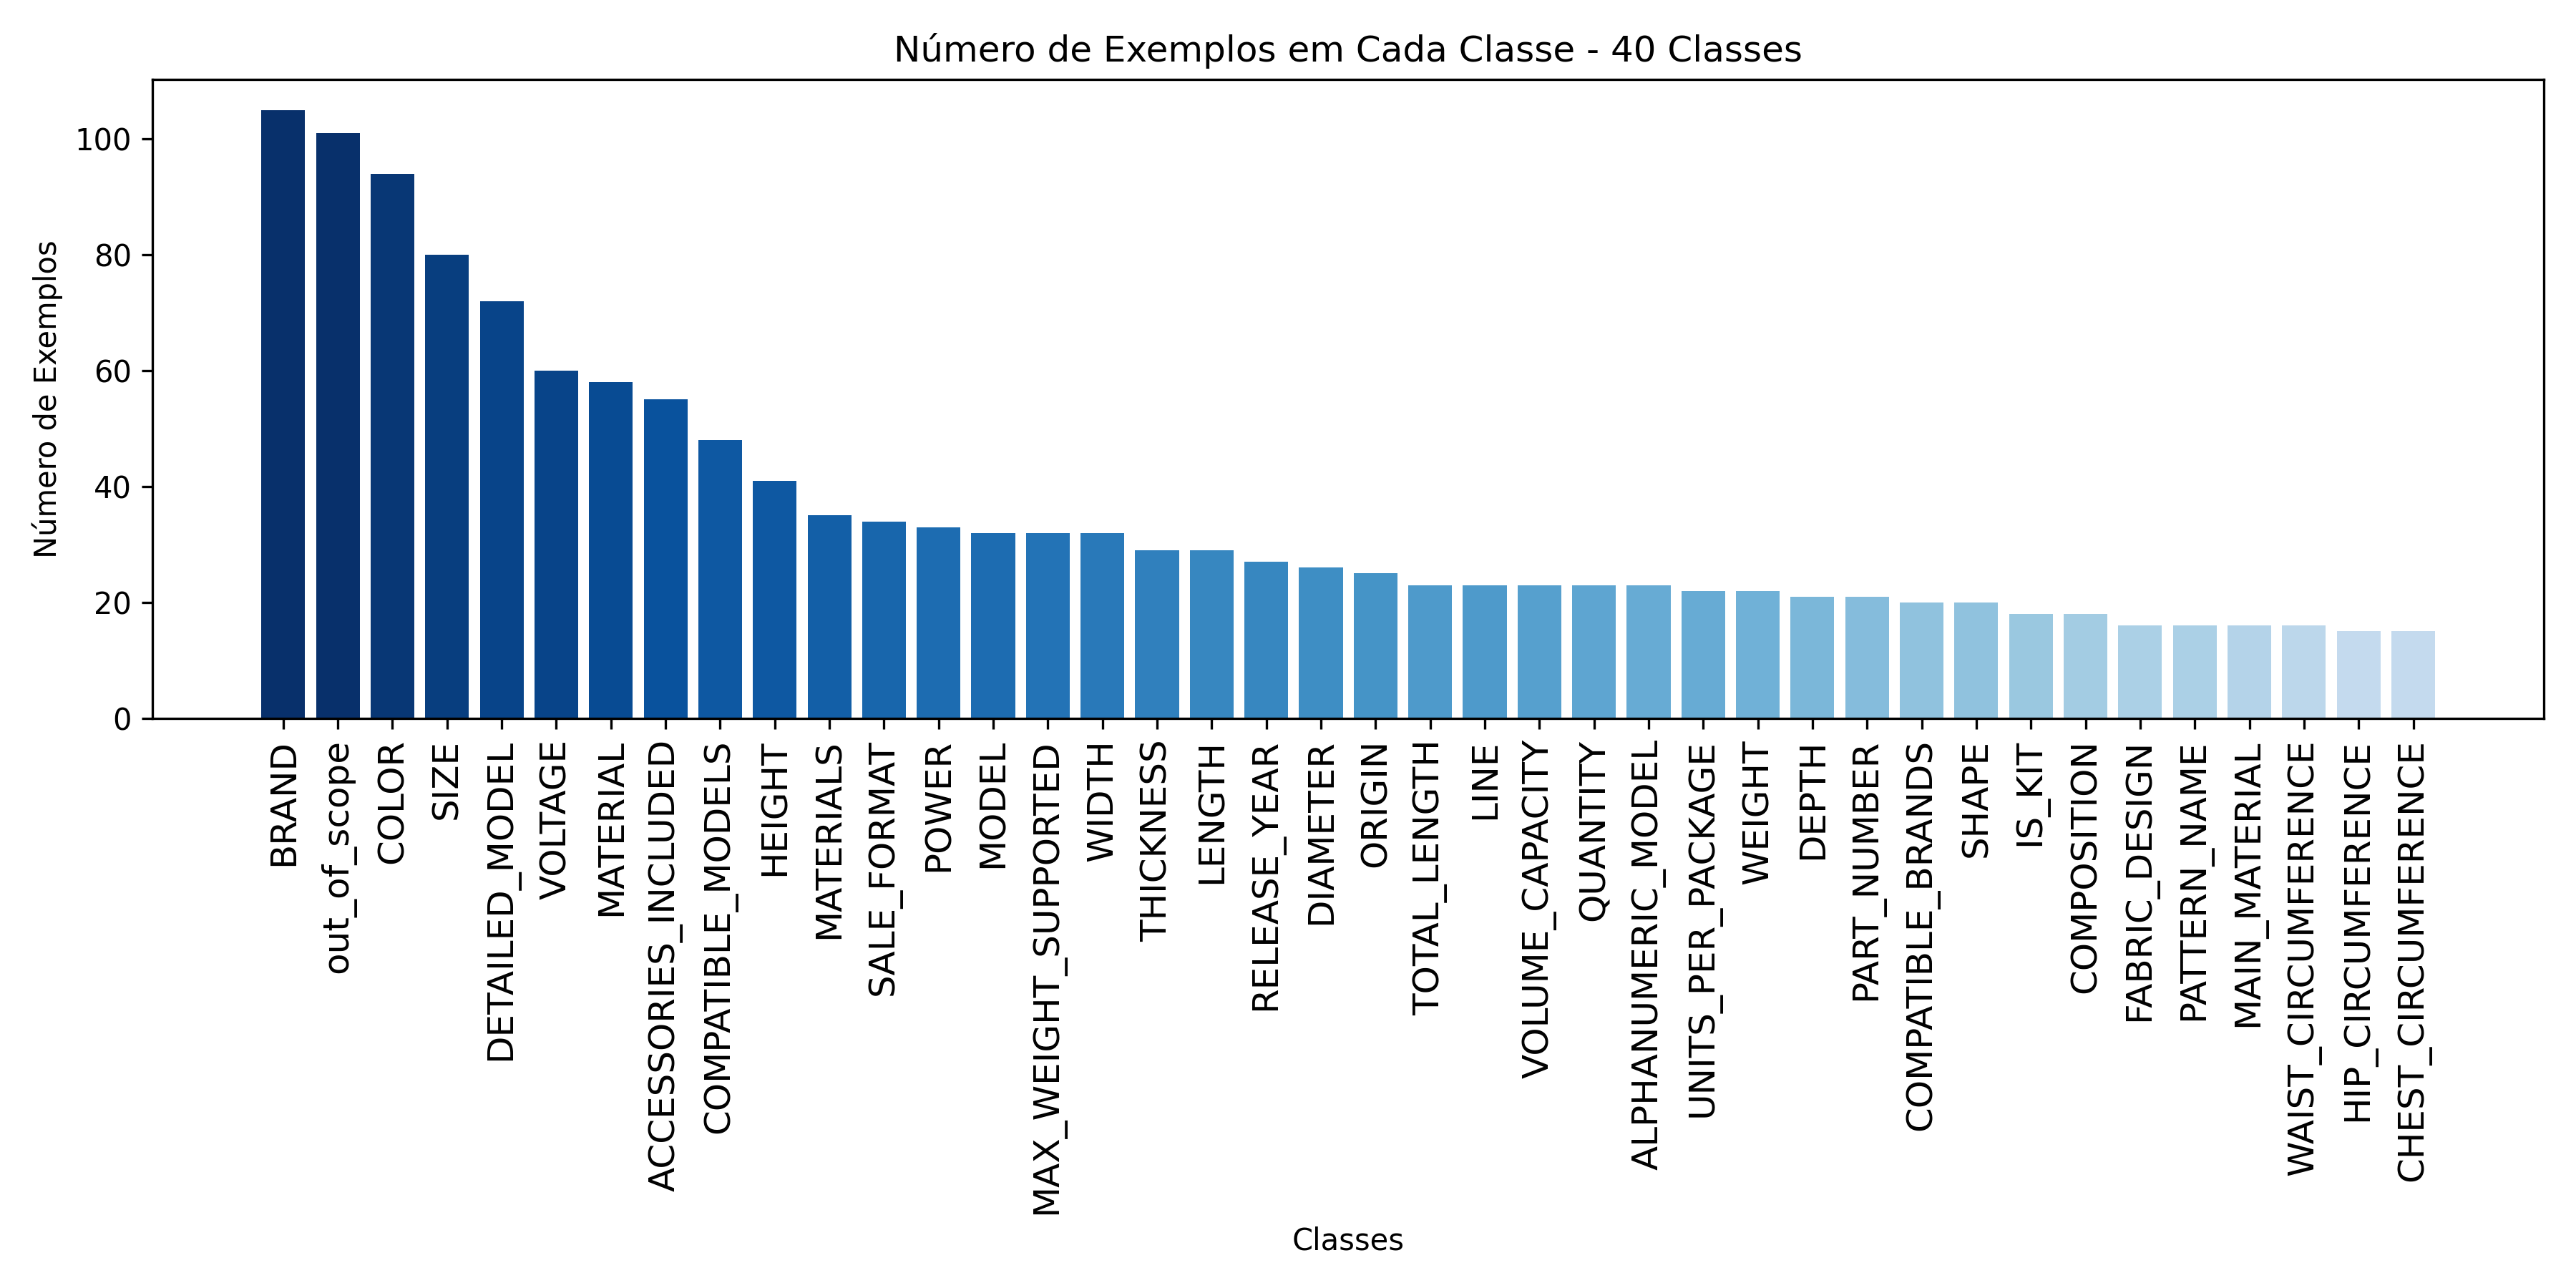
\includegraphics[width=1\linewidth]{figuras/número_de_exemplos_40_classes.png}
	\caption{Gráfico de Barras retratando o número total de exemplos rotulados para cada uma das 40 classes, da classe com mais exemplos para a com menos exemplos.}
	\label{fig:número_de_exemplos_40_classes}
\end{figure}

Para a segunda rodada de criação da base de dados rotulada, foi criada uma nova base de dados, com 28 classes. A quantidade de exemplos de cada classe está descrita na Tabela \ref{table:nova_divisão_de_classes} e as aglutinações de classes feitas foram ilustradas na Figura \ref{fig:aglutinacao_classes}. 

\begin{table}[!ht]
\caption{Quantidade de exemplos rotulados para cada classe na configuração com 28 classes}
\label{table:nova_divisão_de_classes}
\tiny % Define o tamanho da fonte para small (opcional)
\begin{tabularx}{\textwidth}{|X|c|X|c|}
 \hline
 \textbf{Classe} & \textbf{Exemplos} & \textbf{Classe} & \textbf{Exemplos} \\
 \hline
 BRAND & \textbf{105} & MODEL & \textbf{127} \\
 \hline
 COLOR & \textbf{94} & PART\_NUMBER & \textbf{21} \\
 \hline
 MATERIAL & \textbf{127} & LINE & \textbf{23} \\
 \hline
 ORIGIN & \textbf{25} & RELEASE\_YEAR & \textbf{27} \\
 \hline
 WEIGHT & \textbf{22} & QUANTITY & \textbf{97} \\
 \hline
 VOLTAGE & \textbf{60} & SIZE & \textbf{205} \\
 \hline
 DIAMETER & \textbf{26} & DEPTH & \textbf{21} \\
 \hline
 FABRIC\_DESIGN & \textbf{16} & POWER & \textbf{33} \\
 \hline
 PATTERN\_NAME & \textbf{16} & ACCESSORIES\_INCLUDED & \textbf{55} \\
 \hline
 THICKNESS & \textbf{29} & WAIST\_CIRCUMFERENCE & \textbf{16} \\
 \hline
 VOLUME\_CAPACITY & \textbf{23} & HIP\_CIRCUMFERENCE & \textbf{15} \\
 \hline
 COMPATIBLE\_BRANDS & \textbf{20} & SHAPE & \textbf{20} \\
 \hline
 MAX\_WEIGHT\_SUPPORTED & \textbf{32} & CHEST\_CIRCUMFERENCE & \textbf{15} \\
 \hline
 COMPATIBLE\_MODELS & \textbf{48} & out\_of\_scope & \textbf{101} \\
 \hline
 \multicolumn{3}{|l|}{\textbf{Total de Exemplos}} & \textbf{1419} \\
 \hline
\end{tabularx}
\end{table}
% Gráfico de barras - 28 classes
% Criação da Base Rotulada: nuvem de palavras sobre os atributos (classes) com o maior número de exemplos. É uma boa para mostrar o desbalanceamento da base de dados.

A partir da Tabela \ref{table:nova_divisão_de_classes}, é possível perceber que o problema de desbalanceamento de classes se acentuou ainda mais por causa da aglutinação. Isso pode ocasionar um efeito negativo nas métricas de avaliação e será analisado nas seções posteriores. Contudo, o objetivo principal de minimizar a ocorrência de situações em que uma pergunta poderia ser classificada em mais de um atributo ao mesmo tempo foi atingido. Além disso, nenhum exemplo foi removido da base de dados. A Figura \ref{fig:número_de_exemplos_28_classes} retrata, por meio de um gráfico de barras, o número de exemplos rotulados em cada classe nessa configuração com 28 classes.

\begin{figure}[!htb]
    \centering
	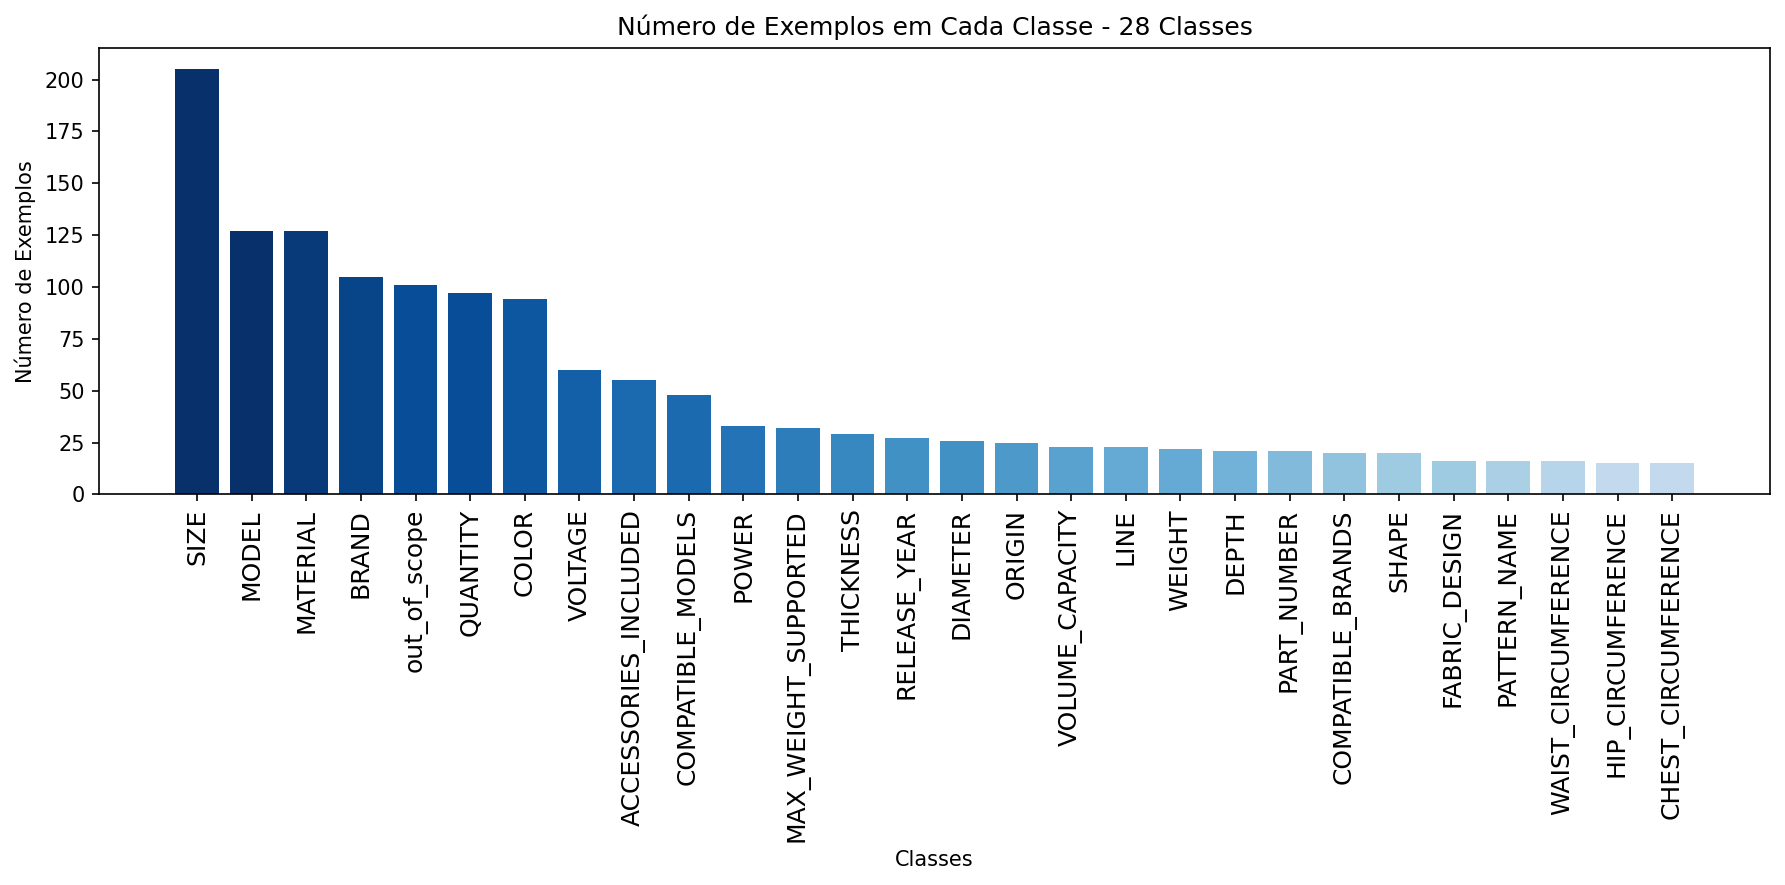
\includegraphics[width=1\linewidth]{figuras/número_de_exemplos_28_classes.png}
	\caption{Gráfico de Barras retratando o número total de exemplos rotulados para cada uma das 28 classes, da classe com mais exemplos para a com menos exemplos.}
	\label{fig:número_de_exemplos_28_classes}
\end{figure}

Analisando a Figura \ref{fig:número_de_exemplos_28_classes}, é possível perceber que \textbf{SIZE} (tamanho) passou a ser a classe com o maior número de exemplos. \textbf{BRAND} (marca), que na primeira rodada da criação da base de dados rotulada era a classe com o maior número de exemplos, passou a ser apenas a 4\textsuperscript{a} maior classe. Outras classes resultantes de aglutinação, \textbf{MODEL} (modelo), \textbf{MATERIAL} (material), e \textbf{QUANTITY} (quantidade), passaram a ser a 2\textsuperscript{a}, 3\textsuperscript{a}, e 6\textsuperscript{a} maior classe, respectivamente. Pelo fato de possuírem um maior número de exemplos quando considerando a base de dados com 28 classes, espera-se que as medidas de avaliação dos modelos classificadores nessas classes aglutinadas sejam melhoradas.


\section{Treinamento e Avaliação dos Classificadores}
\label{res:treinamento_avaliacao_dos_classificadores}
A seguir, será apresentada uma discussão quanto ao desempenho individual de cada um dos algoritmos de classificação treinados, em cada uma das configurações apresentadas. Em um primeiro momento, serão apresentados os resultados dos experimentos envolvendo a base de dados com 40 classes. Em seguida, serão apresentados os resultados dos experimentos envolvendo a base de dados com classes aglutinadas, de 28 classes. 

\subsection{Configuração do Treinamento e Método de Avaliação}
A Tabela \ref{table:divisão_de_classes_com_validação} mostra o número de exemplos de Treino e Teste em cada classe na primeira rodada de experimentos, de 40 classes, enquanto a Tabela \ref{table:nova_divisão_de_classes_com_validação} mostra o número de exemplos de Treino e Teste em cada classe na segunda rodada de experimentos, de 28 classes.

\begin{table}[ht]
\caption{Quantidade de exemplos de Treino e Teste para cada classe na configuração com 40 classes}
\label{table:divisão_de_classes_com_validação}
\tiny % Define o tamanho da fonte para small (opcional)
\begin{tabularx}{\textwidth}{|X|c|c|c|} 
 \hline
 \textbf{Classe} & \textbf{Exemplos de Treino} & \textbf{Exemplos de Teste} & \textbf{Total de Exemplos} \\
 \hline
 BRAND & 84 & 21 & \textbf{105}\\
 \hline
 MODEL & 26 & 6 & \textbf{32}\\
 \hline
 IS\_KIT & 14 & 4 & \textbf{18}\\
 \hline
 COLOR & 75 & 19 & \textbf{94}\\
 \hline
 WIDTH & 25 & 7 & \textbf{32}\\
 \hline
 LENGTH & 23 & 6 & \textbf{29}\\
 \hline
 PART\_NUMBER & 16 & 5 & \textbf{21}\\
 \hline
 MATERIAL & 46 & 12 & \textbf{58}\\
 \hline
 HEIGHT & 32 & 9 & \textbf{41}\\
 \hline
 LINE & 19 & 4 & \textbf{23}\\
 \hline
 UNITS\_PER\_PACKAGE & 18 & 4 & \textbf{22}\\
 \hline
 ORIGIN & 20 & 5 & \textbf{25}\\
 \hline
 RELEASE\_YEAR & 22 & 5 & \textbf{27}\\
 \hline
 WEIGHT & 17 & 5 & \textbf{22}\\
 \hline
 QUANTITY & 18 & 5 & \textbf{23}\\
 \hline
 VOLTAGE & 48 & 12 & \textbf{60}\\
 \hline
 SIZE & 64 & 16 & \textbf{80}\\
 \hline
 DIAMETER & 21 & 5 & \textbf{26}\\
 \hline
 DEPTH & 17 & 4 & \textbf{21}\\
 \hline
 FABRIC\_DESIGN & 12 & 4 & \textbf{16}\\
 \hline
 POWER & 26 & 7 & \textbf{33}\\
 \hline
 COMPOSITION & 15 & 3 & \textbf{18}\\
 \hline
 PATTERN\_NAME & 13 & 3 & \textbf{16}\\
 \hline
 TOTAL\_LENGTH & 19 & 4 & \textbf{23}\\
 \hline
 DETAILED\_MODEL & 58 & 14 & \textbf{72}\\
 \hline
 ACCESSORIES\_INCLUDED & 44 & 11 & \textbf{55}\\
 \hline
 MAIN\_MATERIAL & 13 & 3 & \textbf{16}\\
 \hline
 THICKNESS & 23 & 6 & \textbf{29}\\
 \hline
 MATERIALS & 28 & 7 & \textbf{35}\\
 \hline
 WAIST\_CIRCUMFERENCE & 13 & 3 & \textbf{16}\\
 \hline
 VOLUME\_CAPACITY & 18 & 5 & \textbf{23}\\
 \hline
 HIP\_CIRCUMFERENCE & 12 & 3 & \textbf{15}\\
 \hline
 ALPHANUMERIC\_MODEL & 18 & 5 & \textbf{23}\\
 \hline
 COMPATIBLE\_BRANDS & 16 & 4 & \textbf{20}\\
 \hline
 SHAPE & 16 & 4 & \textbf{20}\\
 \hline
 SALE\_FORMAT & 28 & 6 & \textbf{34}\\
 \hline
 MAX\_WEIGHT\_SUPPORTED & 26 & 6 & \textbf{32}\\
 \hline
 CHEST\_CIRCUMFERENCE & 12 & 3 & \textbf{15}\\
 \hline
 COMPATIBLE\_MODELS & 39 & 9 & \textbf{48}\\
 \hline
 out\_of\_scope & 81 & 20 & \textbf{101}\\
 \hline
 \textbf{Total} & \textbf{1135} & \textbf{284} & \textbf{1419}\\
 \hline
\end{tabularx}
\end{table}

\begin{table}[H]
\caption{Quantidade de exemplos de Treino e Teste para cada classe na configuração com 28 classes}
\label{table:nova_divisão_de_classes_com_validação}
\tiny % Define o tamanho da fonte para small (opcional)
\begin{tabularx}{\textwidth}{|X|c|c|c|} 
 \hline
 \textbf{Classe} & \textbf{Exemplos de Treino} & \textbf{Exemplos de Teste} & \textbf{Total de Exemplos} \\
 \hline
 BRAND & 84 & 21 & \textbf{105}\\
 \hline
 MODEL & 102 & 25 & \textbf{127}\\
 \hline
 COLOR & 75 & 19 & \textbf{94}\\
 \hline
 PART\_NUMBER & 16 & 5 & \textbf{21}\\
 \hline
 MATERIAL & 102 & 25 & \textbf{127}\\
 \hline
 LINE & 19 & 4 & \textbf{23}\\
 \hline
 ORIGIN & 20 & 5 & \textbf{25}\\
 \hline
 RELEASE\_YEAR & 22 & 5 & \textbf{27}\\
 \hline
 WEIGHT & 17 & 5 & \textbf{22}\\
 \hline
 QUANTITY & 78 & 19 & \textbf{97}\\
 \hline
 VOLTAGE & 48 & 12 & \textbf{60}\\
 \hline
 SIZE & 163 & 42 & \textbf{205}\\
 \hline
 DIAMETER & 21 & 5 & \textbf{26}\\
 \hline
 DEPTH & 17 & 4 & \textbf{21}\\
 \hline
 FABRIC\_DESIGN & 12 & 4 & \textbf{16}\\
 \hline
 POWER & 26 & 7 & \textbf{33}\\
 \hline
 PATTERN\_NAME & 13 & 3 & \textbf{16}\\
 \hline
 ACCESSORIES\_INCLUDED & 44 & 11 & \textbf{55}\\
 \hline
 THICKNESS & 23 & 6 & \textbf{29}\\
 \hline
 WAIST\_CIRCUMFERENCE & 13 & 3 & \textbf{16}\\
 \hline
 VOLUME\_CAPACITY & 18 & 5 & \textbf{23}\\
 \hline
 HIP\_CIRCUMFERENCE & 12 & 3 & \textbf{15}\\
 \hline
 COMPATIBLE\_BRANDS & 16 & 4 & \textbf{20}\\
 \hline
 SHAPE & 16 & 4 & \textbf{20}\\
 \hline
 MAX\_WEIGHT\_SUPPORTED & 26 & 6 & \textbf{32}\\
 \hline
 CHEST\_CIRCUMFERENCE & 12 & 3 & \textbf{15}\\
 \hline
 COMPATIBLE\_MODELS & 39 & 9 & \textbf{48}\\
 \hline
 out\_of\_scope & 81 & 20 & \textbf{101}\\
 \hline
 \textbf{Total} & \textbf{1135} & \textbf{284} & \textbf{1419}\\
 \hline
\end{tabularx}
\end{table}


\subsection{Experimentos com 40 Classes}
\label{res:experimentos_40classes}
As Tabelas \ref{tab:metricas_maximas_40classes} e \ref{tab:metricas_gerais_40classes} apresentam os resultados da primeira rodada de experimentos, que usou a base de dados com 40 classes. A Tabela \ref{tab:metricas_maximas_40classes} mostra o número de classes que atingiram o valor máximo de Revocação e Precisão, assim como o número de classes que atingiram o valor mínimo dessas métricas. A Tabela \ref{tab:metricas_gerais_40classes} traz um sumário das métricas de avaliação de cada modelo ponderadas pelo número de exemplos em cada classe. Os modelos estão identificados com os nomes definidos nas Seções \ref{des_treinamento_hf} e \ref{des_treinamento_rasa}. As Matrizes de Confusão estão dispostas no Apêndice \ref{ap:matrizes_de_confusao}.

É possível perceber pela Tabela \ref{tab:metricas_maximas_40classes} que o modelo no qual mais classes tiveram todos os seus exemplos corretamente previstos foi o modelo HF2. Ao mesmo tempo, esse modelo se destacou negativamente pelo fato de não ter previsto corretamente nenhum exemplo de 6 classes, o que indica que o modelo confunde essas classes com outras classes que apresentam exemplos similares.

O modelo que apresentou nos testes o maior número de classes com Precisão igual a 1 foi o modelo HF1. Esse resultado indica que é possível ter grande confiança nesse modelo quando ele prevê que uma pergunta é de determinada classe, ao menos para as classes que apresentaram o valor máximo de Precisão.

Ao prever corretamente ao menos 1 exemplo de Teste para todas as classes, o modelo RASA1 se mostrou um modelo generalista, ou seja, com habilidade de aprender características de todas as classes. Os outros modelos que possuem como algoritmo de classificação o modelo DIETClassifier apresentaram resultados próximos.

\begin{table}[!ht]
\centering
\caption{Número de classes que atingiram o valor máximo e o valor mínimo das métricas de avaliação (base de dados com 40 classes)}
\label{tab:metricas_maximas_40classes}
\resizebox{\textwidth}{!}{%
\begin{tabular}{|c|c|c|c|c|}
\hline
\textbf{ID} & \textbf{Revocação = 1} & \textbf{Precisão = 1} & \textbf{Revocação = 0 e Precisão = 0} \\
\hline
HF1 & 10 & \textbf{16} & 4 \\
\hline
HF2 & \textbf{16} & 13 & 6 \\
\hline 
RASA1 & 10 & 12 & \textbf{0} \\
\hline
RASA2 & 9 & 14 & 1 \\
\hline
RASA3 & 12 & 12 & 1 \\
\hline
\end{tabular}
}
\end{table}

A Tabela \ref{tab:metricas_gerais_40classes} mostra que o modelo HF2 obteve os melhores resultados gerais, apesar do grande número de classes em que nenhum exemplo foi corretamente previsto. Os resultados mostram que esse modelo se mostrou um modelo especialista em algumas classes. Por esse motivo, ele foi o modelo BERT escolhido para os experimentos com a base de dados aglutinada. O modelo RASA3 se destacou em relação à Precisão e por isso foi o modelo DIETClassifier escolhido. 

\begin{table}[!ht]
\centering
\caption{Métricas de avaliação ponderadas pelo número de exemplos de cada classe (base de dados com 40 classes)}
\label{tab:metricas_gerais_40classes}
\resizebox{\textwidth}{!}{%
\begin{tabular}{|c|c|c|c|c|c|c|}
\hline
\textbf{ID} & \textbf{Encoder} & \textbf{Classificador} & \textbf{Acurácia} & \textbf{F1-Score} & \textbf{Precisão} & \textbf{Revocação} \\
\hline
HF1 & BERTimbau & BERTimbau & 0,702 & 0,669 & 0,686 & 0,702 \\
\hline
HF2 & BERTimbau & BERTimbau & \textbf{0,749} & \textbf{0,720} & 0,720 & \textbf{0,749} \\
\hline
RASA1 & BERT-Multi & DIET & 0,680 & 0,668 & 0,705 & 0,680 \\
\hline
RASA2 & BERTimbau & DIET & 0,687 & 0,673 & 0,700 & 0,687 \\
\hline
RASA3 & BERTimbau & DIET & 0,718 & 0,711 & \textbf{0,731} & 0,718 \\
\hline
\end{tabular}}
\end{table}

A Tabela \ref{tab:melhores_classes_revocação_40_classes} sumariza as classes que obtiveram os melhores desempenhos na medida Revocação. Todas as classes mostradas obtiveram desempenho máximo, ou seja, todos os seus exemplos de Teste foram corretamente classificados. Uma característica em comum entre essas classes é que seus exemplos são compostos por palavras ou termos frequentemente repetidos, o que facilita a predição.

\begin{table}[!ht]
\centering
\caption{Classes com os maiores valores de Revocação (base de dados com 40 classes)}
\label{tab:melhores_classes_revocação_40_classes}
\resizebox{\textwidth}{!}{%
\begin{tabular}{|c|c|c|c|c|c|c|c|}
\hline
\textbf{Posição} & \textbf{Classe} & \textbf{HF1} & \textbf{HF2} & \textbf{RASA1} & \textbf{RASA2} & \textbf{RASA3} & \textbf{Média} \\
\hline
1° & DEPTH & 1,000 & 1,000 & 1,000 & 1,000 & 1,000 & 1,000 \\
\hline
1° & HIP\_CIRCUMFERENCE & 1,000 & 1,000 & 1,000 & 1,000 & 1,000 & 1,000 \\
\hline
1° & THICKNESS & 1,000 & 1,000 & 1,000 & 1,000 & 1,000 & 1,000 \\
\hline
1° & VOLTAGE & 1,000 & 1,000 & 1,000 & 1,000 & 1,000 & 1,000 \\
\hline
1° & VOLUME\_CAPACITY & 1,000 & 1,000 & 1,000 & 1,000 & 1,000 & 1,000 \\
\hline
1° & WAIST\_CIRCUNFERENCE & 1,000 & 1,000 & 1,000 & 1,000 & 1,000 & 1,000 \\
\hline
\end{tabular}}
\end{table}

A Tabela \ref{tab:piores_classes_revocação_40_classes} sumariza as classes que obtiveram os piores desempenhos na medida Revocação, ou seja, as classes em que percentualmente menos exemplos de Teste foram classificados corretamente. É possível perceber que 4 das 5 classes apresentadas são compostas de exemplos que poderiam ser classificados em mais de uma classe ao mesmo tempo na ausência de informações complementares, situação que o procedimento de aglutinação de classes tenta resolver. \textbf{COMPATIBLE\_BRANDS}, no entanto, representa um problema maior: ela é uma classe que foi confundida com \textbf{COMPATIBLE\_MODELS} em 4 dos 5 modelos, e um modelo necessitaria de conhecimento de mundo para poder classificá-la corretamente.

\begin{table}[!ht]
\centering
\caption{Classes com os piores valores de Revocação (base de dados com 40 classes)}
\label{tab:piores_classes_revocação_40_classes}
\resizebox{\textwidth}{!}{%
\begin{tabular}{|c|c|c|c|c|c|c|c|}
\hline
\textbf{Posição} & \textbf{Classe} & \textbf{HF1} & \textbf{HF2} & \textbf{RASA1} & \textbf{RASA2} & \textbf{RASA3} & \textbf{Média} \\
\hline
40° & COMPATIBLE\_BRANDS & 0,0000 & 0,0000 & 0,5000 & 0,0000 & 0,0000 & 0,1000 \\
\hline
39° & ALPHANUMERIC\_MODEL & 0,0000 & 0,0000 & 0,2000 & 0,2000 & 0,6000 & 0,2000 \\
\hline
38° & UNITS\_PER\_PACKAGE & 0,0000 & 0,0000 & 0,2500 & 0,5000 & 0,5000 & 0,2500 \\
\hline
37° & MATERIALS & 0,1429 & 0,0000 & 0,5714 & 0,4286 & 0,5714 & 0,3429 \\
\hline
36° & MODEL & 0,1667 & 0,3333 & 0,6667 & 0,1667 & 0,5000 & 0,3667 \\
\hline
\end{tabular}}
\end{table}

\subsection{Experimentos com 28 Classes}
As Tabelas \ref{tab:metricas_maximas_28classes} e \ref{tab:metricas_gerais_28classes} apresentam o desempenho dos modelos treinados na base de dados com 28 classes e aglutinações de classes propostas na Seção \ref{criacao_base_dados_rotulada}. Os modelos treinados nessa etapa são iguais aos modelos treinados na etapa anterior. As Matrizes de Confusão estão dispostas no Apêndice \ref{ap:matrizes_de_confusao}.

O resultado mostrado na Tabela \ref{tab:metricas_maximas_28classes} indica que nesse cenário o modelo HF2 performou melhor que o modelo RASA3 em todos os aspectos. A diminuição no número de classes em que os modelos atingiram o valor máximo das métricas de avaliação é naturalmente esperada pela aplicação da aglutinação de classes. O modelo RASA3 apresentou dificuldade em aprender quando classificar um exemplo como \textbf{MODEL}: os exemplos dessa classe foram classificados como pertencentes a 10 classes diferentes.

\begin{table}[!ht]
\centering
\caption{Número de classes que atingiram o valor máximo e o valor mínimo das métricas de avaliação (base de dados com 28 classes)}
\label{tab:metricas_maximas_28classes}
\resizebox{\textwidth}{!}{%
\begin{tabular}{|c|c|c|c|c|}
\hline
\textbf{ID} & \textbf{Revocação = 1} & \textbf{Precisão = 1} & \textbf{Revocação = 0 e Precisão = 0} \\
\hline
HF2 & \textbf{11} & \textbf{11} & \textbf{1} \\
\hline 
RASA3 & \textbf{11} & 7 & \textbf{1} \\
\hline
\end{tabular}
}
\end{table}

A Tabela \ref{tab:metricas_gerais_28classes} confirma o bom desempenho do modelo HF2 quando comparado ao modelo RASA3. Além disso, ela demonstra que a aplicação da aglutinação de classes foi benéfica para os modelos: houve uma melhoria de 14,8\% em Acurácia, de 18,6\% em F1-Score, de 19,7\% em Precisão e de 14,8\% em Revocação no desempenho do modelo HF2 na base de dados com 28 classes em comparação ao desempenho do modelo HF2 na base de dados com 40 classes. O modelo RASA3 também foi influenciado positivamente pelo procedimento, porém com menos intensidade.

\begin{table}[!ht]
\centering
\caption{Métricas de avaliação ponderadas pelo número de exemplos de cada classe (base de dados com 28 classes)}
\label{tab:metricas_gerais_28classes}
\resizebox{\textwidth}{!}{%
\begin{tabular}{|c|c|c|c|c|c|c|}
\hline
\textbf{ID} & \textbf{Encoder} & \textbf{Classificador} & \textbf{Acurácia} & \textbf{F1-Score} & \textbf{Precisão} & \textbf{Revocação} \\
\hline
HF2 & BERTimbau & BERTimbau & \textbf{0,860} & \textbf{0,854} & \textbf{0,862} & \textbf{0,860} \\
\hline
RASA3 & BERTimbau & DIET & 0,763 & 0,755 & 0,775 & 0,763 \\
\hline
\end{tabular}}
\end{table}

A Tabela \ref{tab:melhores_classes_revocação_28_classes} sumariza as classes da base de dados com 28 classes que obtiveram os melhores desempenhos na medida Revocação, ou seja, as classes em que percentualmente mais exemplos de Teste foram classificados corretamente. Mais uma vez, há predomínio de classes consideradas de fácil predição, com exceção de \textbf{ORIGIN}.

\begin{table}[!ht]
\centering
\caption{Classes com os maiores valores de Revocação (base de dados com 28 classes)}
\label{tab:melhores_classes_revocação_28_classes}
\begin{tabular}{|c|c|c|c|c|}
\hline
\textbf{Posição} & \textbf{Classe} & \textbf{HF2} & \textbf{RASA3} & \textbf{Média} \\
\hline
1° & CHEST\_CIRCUMFERENCE & 1,000 & 1,000 & 1,000 \\
\hline
1° & DEPTH & 1,000 & 1,000 & 1,000 \\
\hline
1° & DIAMETER & 1,000 & 1,000 & 1,000 \\
\hline
1° & HIP\_CIRCUMFERENCE & 1,000 & 1,000 & 1,000 \\
\hline
1° & ORIGIN & 1,000 & 1,000 & 1,000 \\
\hline
1° & WAIST\_CIRCUNFERENCE & 1,000 & 1,000 & 1,000 \\
\hline
1° & WEIGHT & 1,000 & 1,000 & 1,000 \\
\hline
\end{tabular}
\end{table}

A Tabela \ref{tab:piores_classes_revocação_28_classes} sumariza as classes que obtiveram os piores desempenhos na medida Revocação. No geral, os modelos apresentaram valores mais altos para essa métrica do que os valores vistos na Tabela \ref{tab:piores_classes_revocação_40_classes}, o que confirma a eficácia da aglutinação de classes. A classe \textbf{MODEL} foi a única entre as classes aglutinadas que continuou na lista das 5 classes com os piores resultados.

A classe \textbf{COMPATIBLE\_BRANDS}, que havia sido a classe com os piores resultados na etapa anterior, continuou a ser a classe em que os modelos mais apresentam dificuldade de predição. A média de pontuação em Revocação era de 0,1000 no experimento anterior. No experimento com 28 classes, essa média caiu para 0,0000. Isso indica que nenhum dos dois modelos que tiveram os melhores desempenhos foi capaz de classificar corretamente 1 pergunta como \textbf{COMPATIBLE\_BRANDS}.

De forma geral, não é possível apontar um modelo mais generalista e um modelo mais especialista entre os modelos treinados na base de dados de 28 classes. Ambos os modelos não conseguiram prever corretamente os exemplos de uma única classe. Sendo assim, como as medidas de avaliação do modelo HF2 descritas na Tabela \ref{tab:metricas_gerais_28classes} apontam um desempenho geral muito superior desse modelo, ele é o melhor modelo treinado considerando as duas rodadas de experimentos.

\begin{table}[!ht]
\centering
\caption{Classes com os piores valores de Revocação (base de dados com 28 classes)}
\label{tab:piores_classes_revocação_28_classes}
\begin{tabular}{|c|c|c|c|c|}
\hline
\textbf{Posição} & \textbf{Classe} & \textbf{HF2} & \textbf{RASA3} & \textbf{Média} \\
\hline
28° & COMPATIBLE\_BRANDS & 0,000 & 0,000 & 0,000 \\
\hline
27° & MAX\_WEIGHT\_SUPPORTED & 0,500 & 0,500 & 0,500 \\
\hline
27° & SHAPE & 0,250 & 0,750 & 0,500 \\
\hline
25° & MODEL & 0,720 & 0,320 & 0,520 \\
\hline
24° & COMPATIBLE\_MODELS & 0,667 & 0,556 & 0,611 \\
\hline
\end{tabular}
\end{table}

\section{Comparativo entre Classes Frequentemente Confundidas}
\label{res:comparativo_entre_classes_confundidas}
As Figuras \ref{fig:compatible_brands} e \ref{fig:compatible_models} apresentam as nuvens de palavras geradas a partir dos exemplos de Treino e de Teste das classes \textbf{COMPATIBLE\_BRANDS} e \textbf{COMPATIBLE\_MODELS}, respectivamente.

É possível perceber que, apesar dessas duas classes serem frequentemente confundidas, as palavras que compõem seus exemplos se repetem pouco entre si. A maior exceção está relacionada à palavra \textbf{compatível}, que aparece 9 vezes nos exemplos da classe \textbf{COMPATIBLE\_BRANDS} e 16 vezes nos exemplos da classe \textbf{COMPATIBLE\_MODELS}.

É possível concluir que um dos motivos para a dificuldade apresentada pelos modelos em classificar corretamente os exemplos da classe \textbf{COMPATIBLE\_BRANDS} é a falta de conhecimento de mundo para entender quais palavras representam marcas e quais palavras representam modelos. Como estatisticamente a palvra \textbf{compatível} aparece mais vezes na classe \textbf{COMPATIBLE\_MODELS}, os modelos esperam que qualquer exemplo que apresente essa palavra também pertença a essa classe. Uma possível solução para esse problema é fazer uso de grandes estruturas de dados que salvem nomes de marcas e de modelos, como o grafo de conhecimento interno do Mercado Livre. Uma solução alternativa que poderia ser testada é o uso de outros modelos de Aprendizado Profundo que possuam um maior número de parâmetros.

\begin{figure}[!ht]
    \centering
	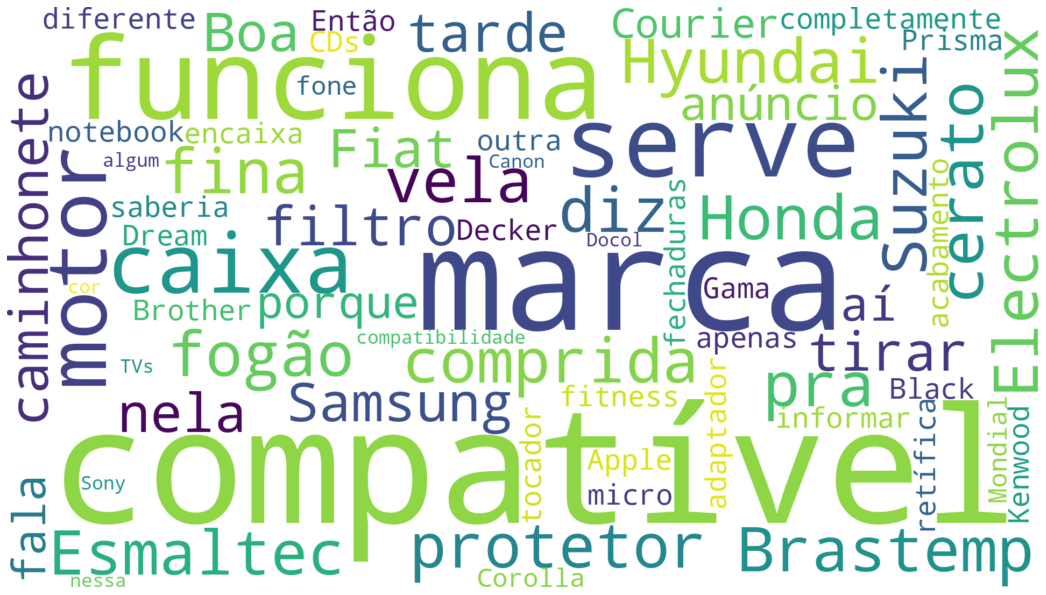
\includegraphics[width=1\linewidth]{figuras/compatible_brands.png}
	\caption{Nuvem de palavras gerada a partir dos exemplos de Treino e Teste da classe \textbf{COMPATIBLE\_BRANDS}, após remoção de \textit{stopwords}.}
	\label{fig:compatible_brands}
\end{figure}

\begin{figure}[!ht]
    \centering
	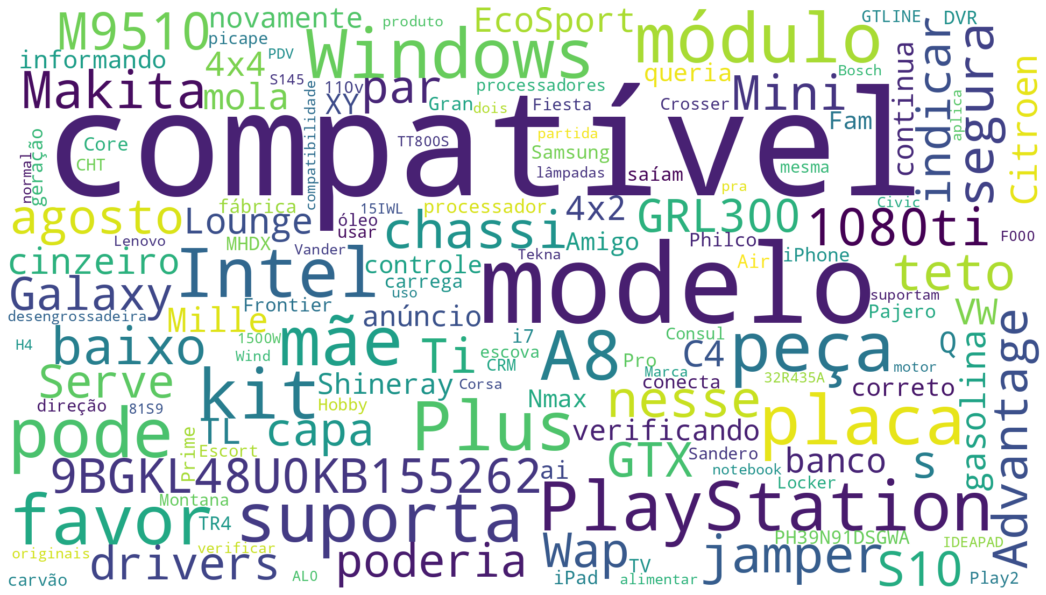
\includegraphics[width=1\linewidth]{figuras/compatible_models.png}
	\caption{Nuvem de palavras gerada a partir dos exemplos de Treino e Teste da classe \textbf{COMPATIBLE\_MODELS}, após remoção de \textit{stopwords}.}
	\label{fig:compatible_models}
\end{figure}

\clearpage % Para garantir que as imagens não irão ser mostradas na próxima Seção
\section{Considerações Finais}
Neste capítulo, uma visão geral dos resultados obtidos em cada etapa do trabalho foi apresentada. Foi feita uma análise da representatividade de cada atributo definido como classe em relação ao número de subcategorias de produtos do Mercado Livre em que esse atributo pode ser utilizado. Além disso, foi realizada uma estimativa da quantidade de dados coletados de cada fonte. Uma análise em relação ao número de exemplos rotulados de cada classe e as condições que levaram ao desbalanceamento entre as classes também foi feita.

Após testes com cinco configurações de modelos classificadores e duas configurações de base de dados, foi possível escolher o modelo HF2 como o melhor algoritmo de classificação. O modelo mostrou ser especialista em algumas classes na configuração de base de dados original, que se aproxima mais do problema real. Em seguida, o modelo foi aplicado sobre a base de dados aglutinada e melhorou substancialmente suas métricas de avaliação, o que indica a eficiência desse procedimento na recategorização de perguntas que poderiam pertencer a mais de uma classe. O modelo RASA3 também apresentou um resultado positivo: foi o segundo melhor modelo de acordo com as métricas de avaliação e se mostrou mais generalista.

A partir dos resultados obtidos, foi possível concluir que o método apresentado é eficaz em classificar corretamente variados tipos de perguntas. No entanto, algumas classes são frequentemente confundidas em todos os modelos testados por falta de conhecimento de mundo. Por isso, avaliações de outras metodologias deveriam ser feitas caso haja interesse em classificar essas classes de forma satisfatória.

% Avaliação dos Classificadores: todas as matrizes de confusão, assim como as tabelas de resultado das duas planilhas. Primeiro apresentar BERT-40classes, depois DIET-40classes, e depois os dois juntos no experimento com 28 classes.

% A comparação RASA1 vs. RASA3 é interessante, uma vez que a única diferença entre as duas pipelines é a etapa de pré-processamento dos dados. Salientar o CountVectorsFeaturizer que se saiu superior. Porém, não me parece natural apresentar esse resultado antes da Avaliação dos Classificadores em si.

% Assim como na página 59 do TCC do Oscar, talvez fazer um ranking das 5 classes mais acertadas pelo HF em porcentagem (para desconsiderar o desbalanceamento)

% Tentar investigar o porquê de classes que tiveram desempenho falho, mesmo no melhor modelo, falharam. Talvez com nuvens de palavras.
% COMPATIBLE_BRANDS: apenas 1 ou outro VERDADEIROS POSITIVOS foram encontrados em todos os testes. É a classe que foi menos acertada (ver qual métrica é essa). Provavelmente foi confundida com COMPATIBLE_MODELS. Comparar as palavras da nuvem de palavras de cada uma para perceber que as palavras são as mesmas e falta conhecimento de mundo. Apresentar como solução para isso o uso do grafo de conhecimento do Mercado Livre do que são MARCAS e do que são MODELOS ou usar modelos com muito mais parâmetros (como as LLMs) sempre que uma pergunta for classificada como COMPATIBLE_X.

% Mostrar que, nas classes que o BERT se sai bem, ele acerta MAIS do que o RASA. No entanto, nas classes em que ambos os modelos se saem mal, o RASA acerta 1 ou outro exemplo. O BERT pode ser especialista, o RASA generalista.






% ----------------------------------------------------------
% Conclusão
% ----------------------------------------------------------
\chapter[Conclusão]{Conclusão}
\label{cap-conclusao}
%TCC:
Este trabalho apresentou uma metodologia para a resolução de dúvidas de clientes reais sobre produtos do comércio eletrônico usando inteligência artificial, desde a etapa de definição das classes até a etapa de medidas e método de avaliação dos classificadores treinados. As disciplinas Algoritmos e Programação de Computadores e Inteligência Artificial, do curso de Graduação em Engenharia Mecatrônica da Universidade Federal de Uberlândia, se mostraram importantes para o entendimento dos conceitos teóricos aplicados na realização deste trabalho.

O Mercado Livre foi a plataforma de comércio eletrônico escolhida, em virtude da grande quantidade de perguntas feitas na plataforma disponível na base de dados da empresa GoBots.

Na prática, a metodologia consiste em tratar a situação como um problema de classificação de texto multi-classe, onde cada classe representa um atributo de produto. A resolução das dúvidas em si é feita após a predição da classe e consulta à API do Mercado Livre pelo nome do atributo inferido. No entanto, o trabalho apresentou um foco maior na etapa anterior à resolução das dúvidas, ou seja, no procedimento de treinamento dos modelos classificadores responsáveis por prever a qual atributo uma pergunta se refere.

Para atingir o objetivo, foram realizadas as seguintes etapas da Classificação de Texto Multi-classe: definição das classes, coleta de dados, criação da base de dados rotulada, pré-processamento dos dados, treinamento dos algoritmos de classificação e medidas e método de avaliação dos classificadores. A abordagem de classificação de texto aplicada na base de dados rotulada foi o uso de dois modelos transformadores, BERT e DIETClassifier, avaliados quanto a diferentes configurações de hiperparâmetros e etapas de pré-processamento. 

Os experimentos foram feitos em duas rodadas. Na primeira rodada, a base de dados se aproxima mais do problema real, pois consiste de 40 classes existentes no Mercado Livre. Nessa rodada, percebeu-se que a arquitetura de transformador que usa o modelo brasileiro BERTimbau Base tanto no pré-processamento quanto na classificação de texto apresentou um desempenho excelente em algumas classes específicas, porém abaixo da média em outras. Ao mesmo tempo, a arquitetura de transformador que usa BERTimbau Base no pré-processamento e DIETClassifier na classificação de texto apresentou um desempenho razoável em todas as classes.

Na segunda rodada de experimentos, a base de dados foi aglutinada para 28 classes com o objetivo de minimizar as situações em que uma pergunta poderia ser classificada em mais de uma classe. Nessa situação, a arquitetura de transformador que usa BERTimbau Base tanto no pré-processamento quanto na classificação de texto se mostrou muito superior.

Considerando a primeira rodada de experimentos, uma boa opção para a resolução de perguntas de clientes reais é aplicar o melhor modelo DIETClassifier e o melhor modelo BERT em paralelo. O primeiro, mais generalista, iria ponderar igualmente a possibilidade da pergunta pertencer a cada uma das classes. O segundo, mais especialista, serviria para verificar a previsão feita pelo primeiro, ao apresentar uma maior certeza quanto a classe a qual a pergunta pertence. Uma forma de se fazer isso frequentemente abordada na literatura é a criação de um mecanismo de votação, no qual os dois modelos classificam a pergunta fornecida ao mesmo tempo e tomam uma decisão em conjunto dependendo da pontuação retornada por cada modelo ao fazer a classificação.

Algumas classes foram destaques negativos por conta da dificuldade dos modelos em aprenderem a identificá-las, em todas as configurações avaliadas. Entre esses destaques estão as classes que descrevem as marcas compatíveis com determinado produto e os modelos compatíveis com determinado produto.

\section{Principais Contribuições}
\begin{itemize}
    \item Elaboração e divulgação de uma metodologia de resolução de dúvidas de clientes reais em plataformas de comércio eletrônico;
    \item Indicação de duas arquiteturas de transformadores que apresentam bom desempenho na tarefa de classificação de perguntas quanto ao atributo de produto ao qual elas se referem;
    \item Divulgação das medidas de avaliação atingidas pelas arquiteturas de transformadores utilizadas, que servem como motivação para que trabalhos futuros busquem melhores resultados;
    \item Criação de uma base de dados rotulada privada, composta por 1419 exemplos de perguntas rotuladas a respeito do atributo de produto ao qual elas se referem.
\end{itemize}

\section{Trabalhos Futuros}
Neste trabalho, foram treinados modelos classificadores de texto de alto desempenho na identificação de múltiplas classes. No entanto, a predição de algumas classes, notadamente as relacionadas com compatibilidade de produtos com marcas e modelos, apresentou resultados negativos.

Para resolver esse problema, outras metodologias podem ser testadas. Entre elas, o uso de grandes estruturas de dados, como os grafos de conhecimento, que armazenam nomes de marcas e nomes de modelos. Uma outra possibilidade é o uso de modelos de aprendizado de máquina de dimensões maiores, como os modelos de linguagem de grande porte, que naturalmente guardam consigo noções de nomes de marcas e nomes de modelos por conta do seu alto número de parâmetros. Além disso, pode ser avaliada a possibilidade de que esses modelos apresentem uma maior facilidade na identificação de como os exemplos de cada classe são estruturados, pelo fato de terem sido treinados em um número muito maior de exemplos.

Uma alternativa para o uso de modelos de aprendizado de máquina de dimensões maiores que também pode ser abordada em trabalhos futuros é o uso de técnicas de \textit{ensemble}, ou seja, fazer a classificação de uma mesma pergunta em modelos diferentes e usar um algoritmo de votação para determinar a resposta correta. O algoritmo de votação pode ser, por exemplo, considerar a classe prevista pela maioria dos modelos como a classe correta.

Outros trabalhos podem apresentar resultados diferentes ao fazer uso de outras formas de pré-processamento. As pessoas frequentemente fazem uso de gírias ou grafias diferentes da norma culta da Língua Portuguesa ao fazer perguntas nos sites de \textit{e-commerce}, e os tokenizadores utilizados neste trabalho não são totalmente eficientes no tratamento dessas situações.




% ----------------------------------------------------------
% ELEMENTOS PÓS-TEXTUAIS
% ----------------------------------------------------------
\postextual


% ----------------------------------------------------------
% Referências bibliográficas
% ----------------------------------------------------------
\bibliography{abntex2-modelo-references}


%% ----------------------------------------------------------
%% Apêndices TCC: só mantenha se for pertinente.
%% ----------------------------------------------------------

% ---
% Inicia os apêndices
% ---
\begin{apendicesenv}

% Imprime uma página indicando o início dos apêndices
\partapendices

% ----------------------------------------------------------
\chapter{Matrizes de Confusão}
\label{ap:matrizes_de_confusao}

\begin{figure}[!ht]
    \centering
	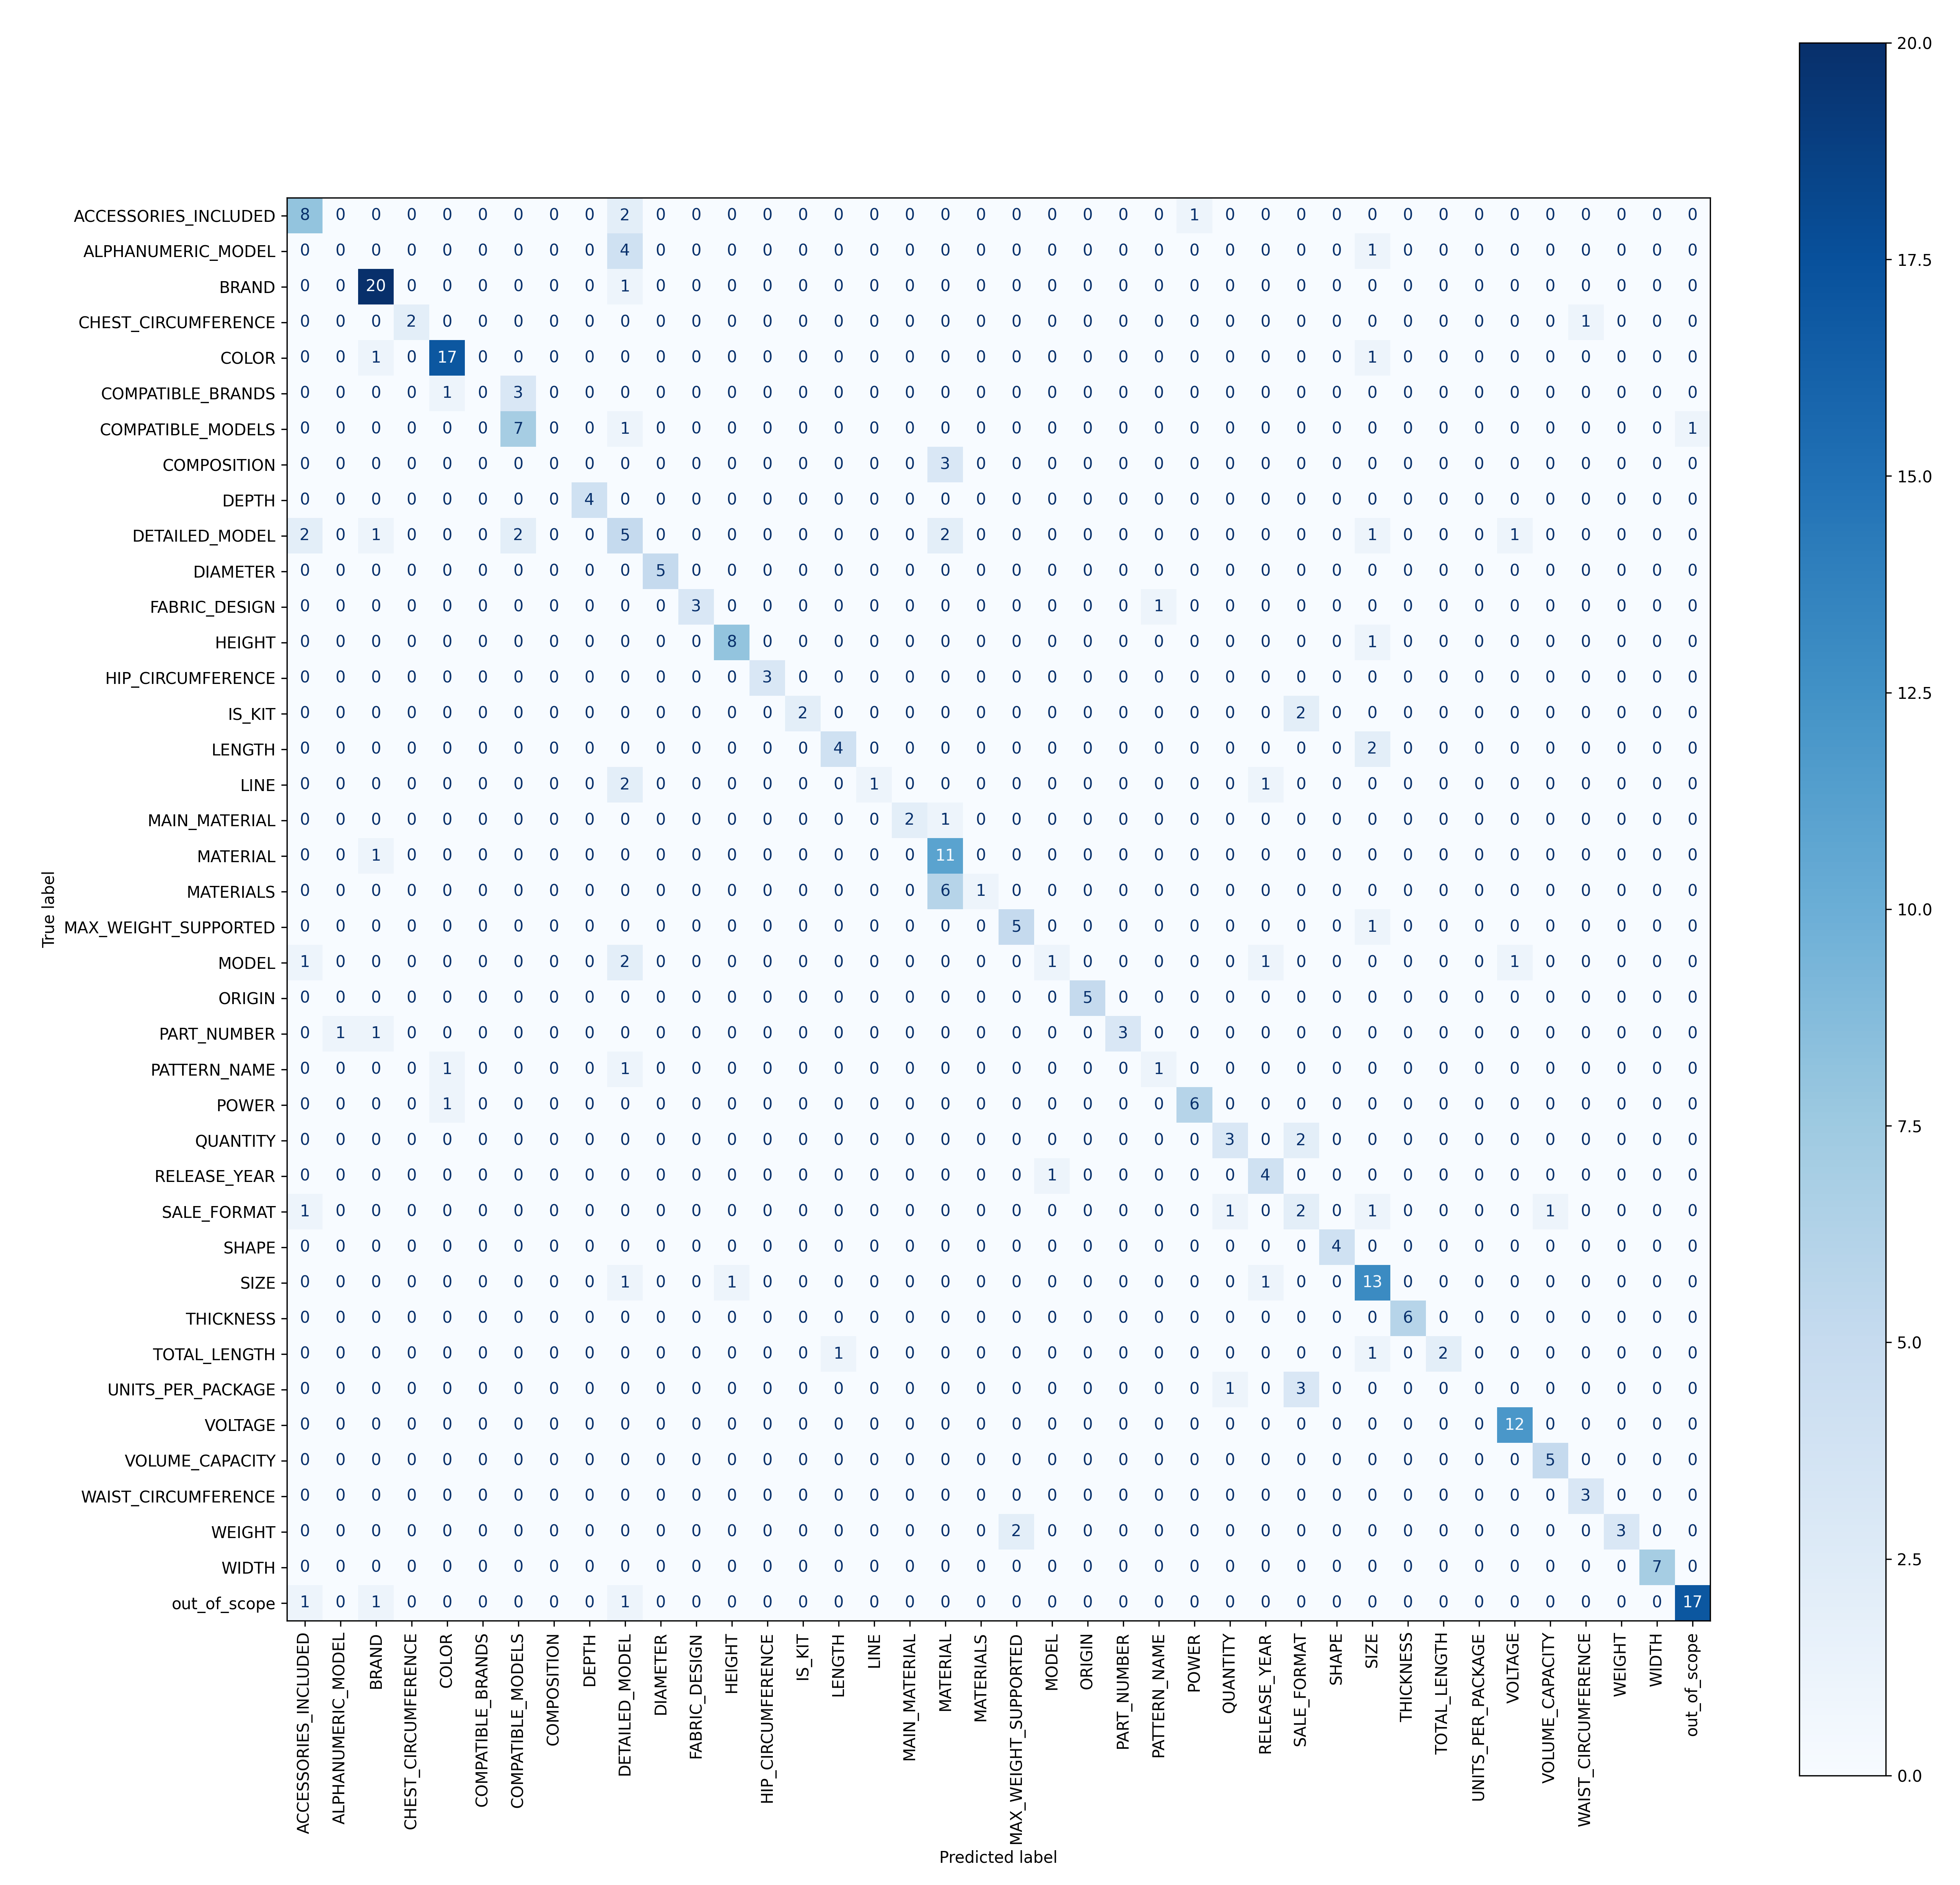
\includegraphics[width=1\linewidth]{figuras/HF1.png}
	\caption{Matriz de Confusão gerada após teste do modelo HF1, na configuração com 40 classes.}
	\label{fig:matriz_hf1}
\end{figure}

\begin{figure}[!ht]
    \centering
	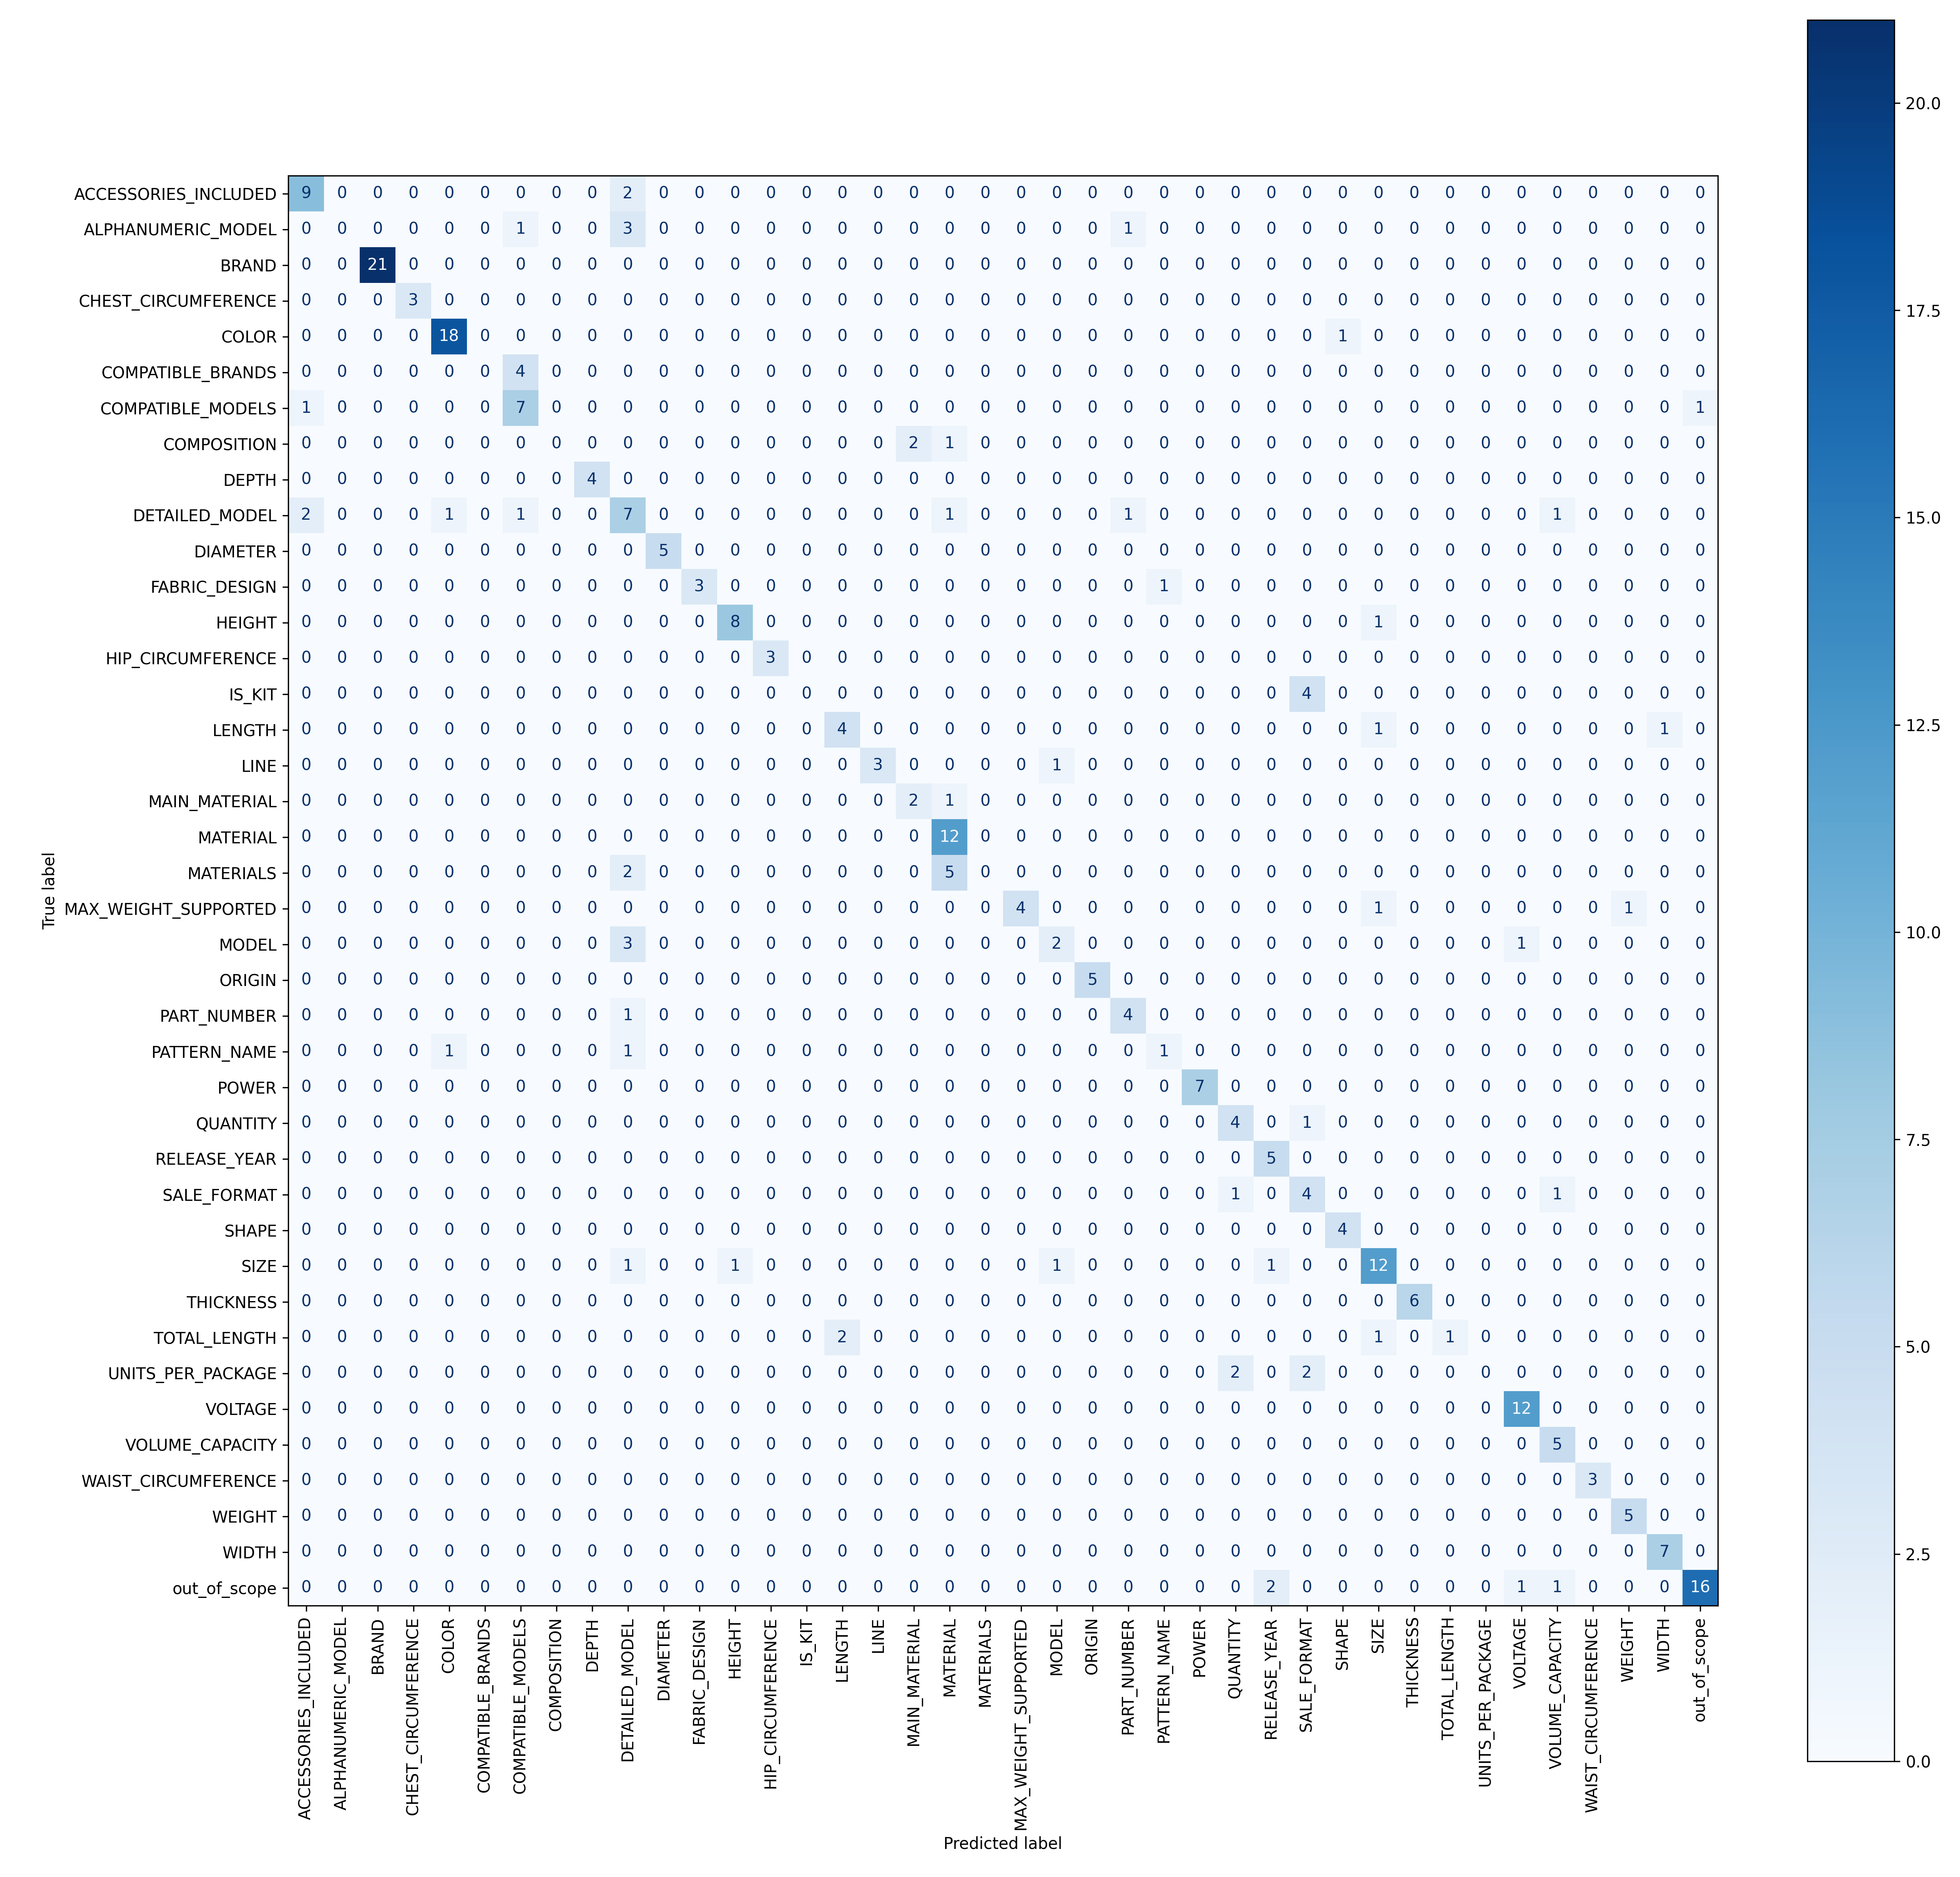
\includegraphics[width=1\linewidth]{figuras/HF2.png}
	\caption{Matriz de Confusão gerada após teste do modelo HF2, na configuração com 40 classes.}
	\label{fig:matriz_hf2}
\end{figure}

\begin{figure}[!ht]
    \centering
	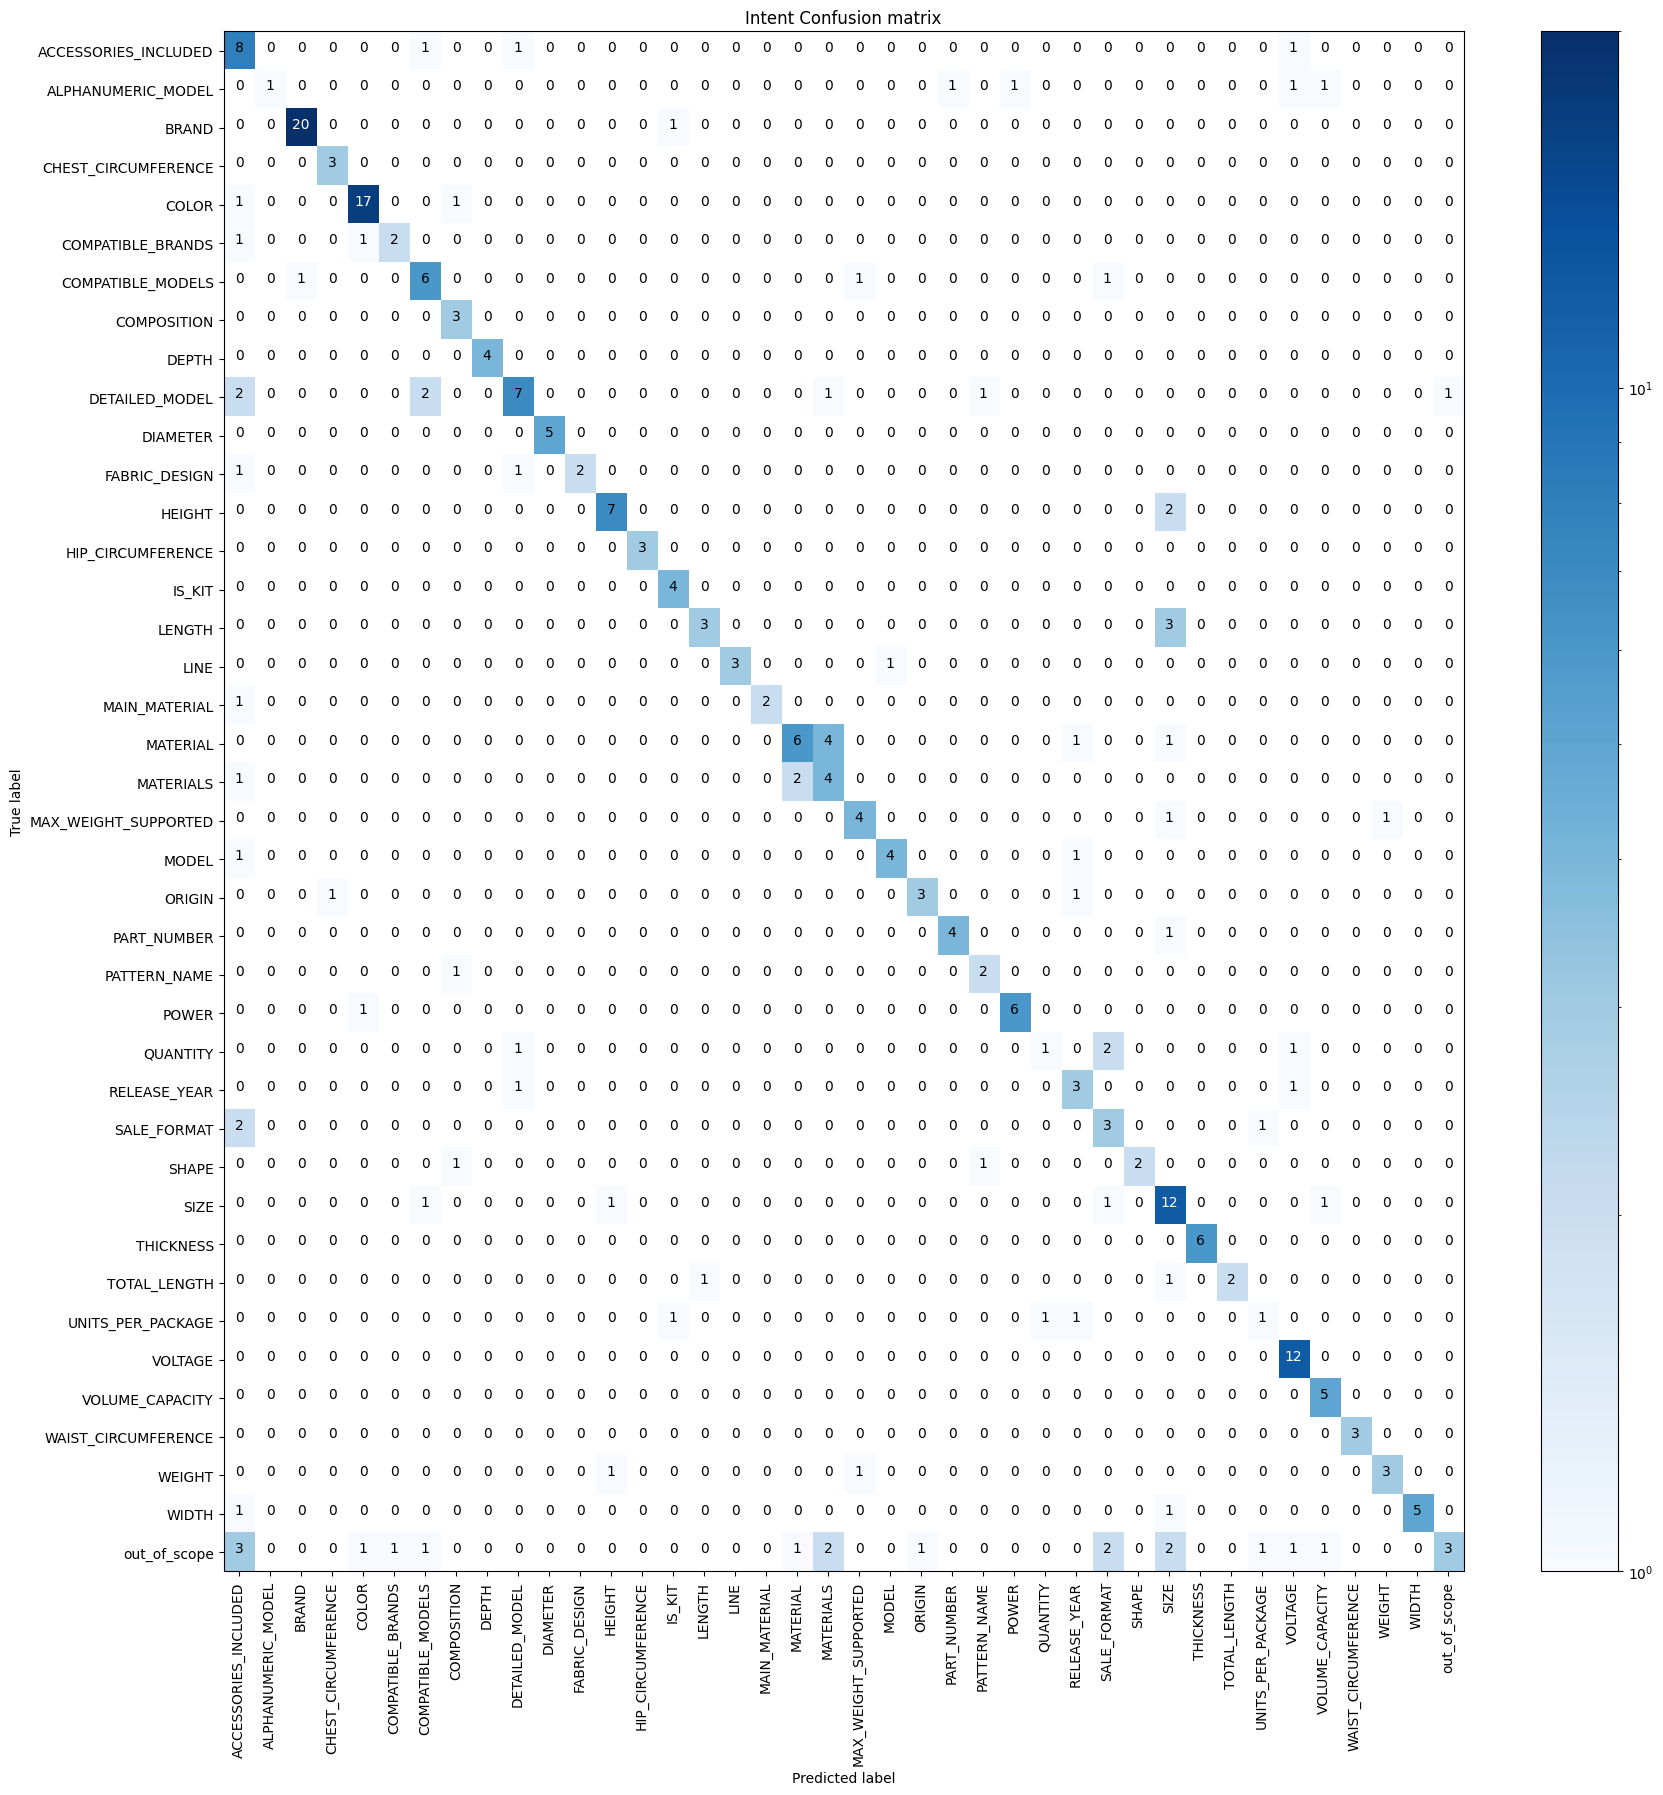
\includegraphics[width=1\linewidth]{figuras/RASA1.png}
	\caption{Matriz de Confusão gerada após teste do modelo RASA1, na configuração com 40 classes.}
	\label{fig:matriz_rasa1}
\end{figure}

\begin{figure}[!ht]
    \centering
	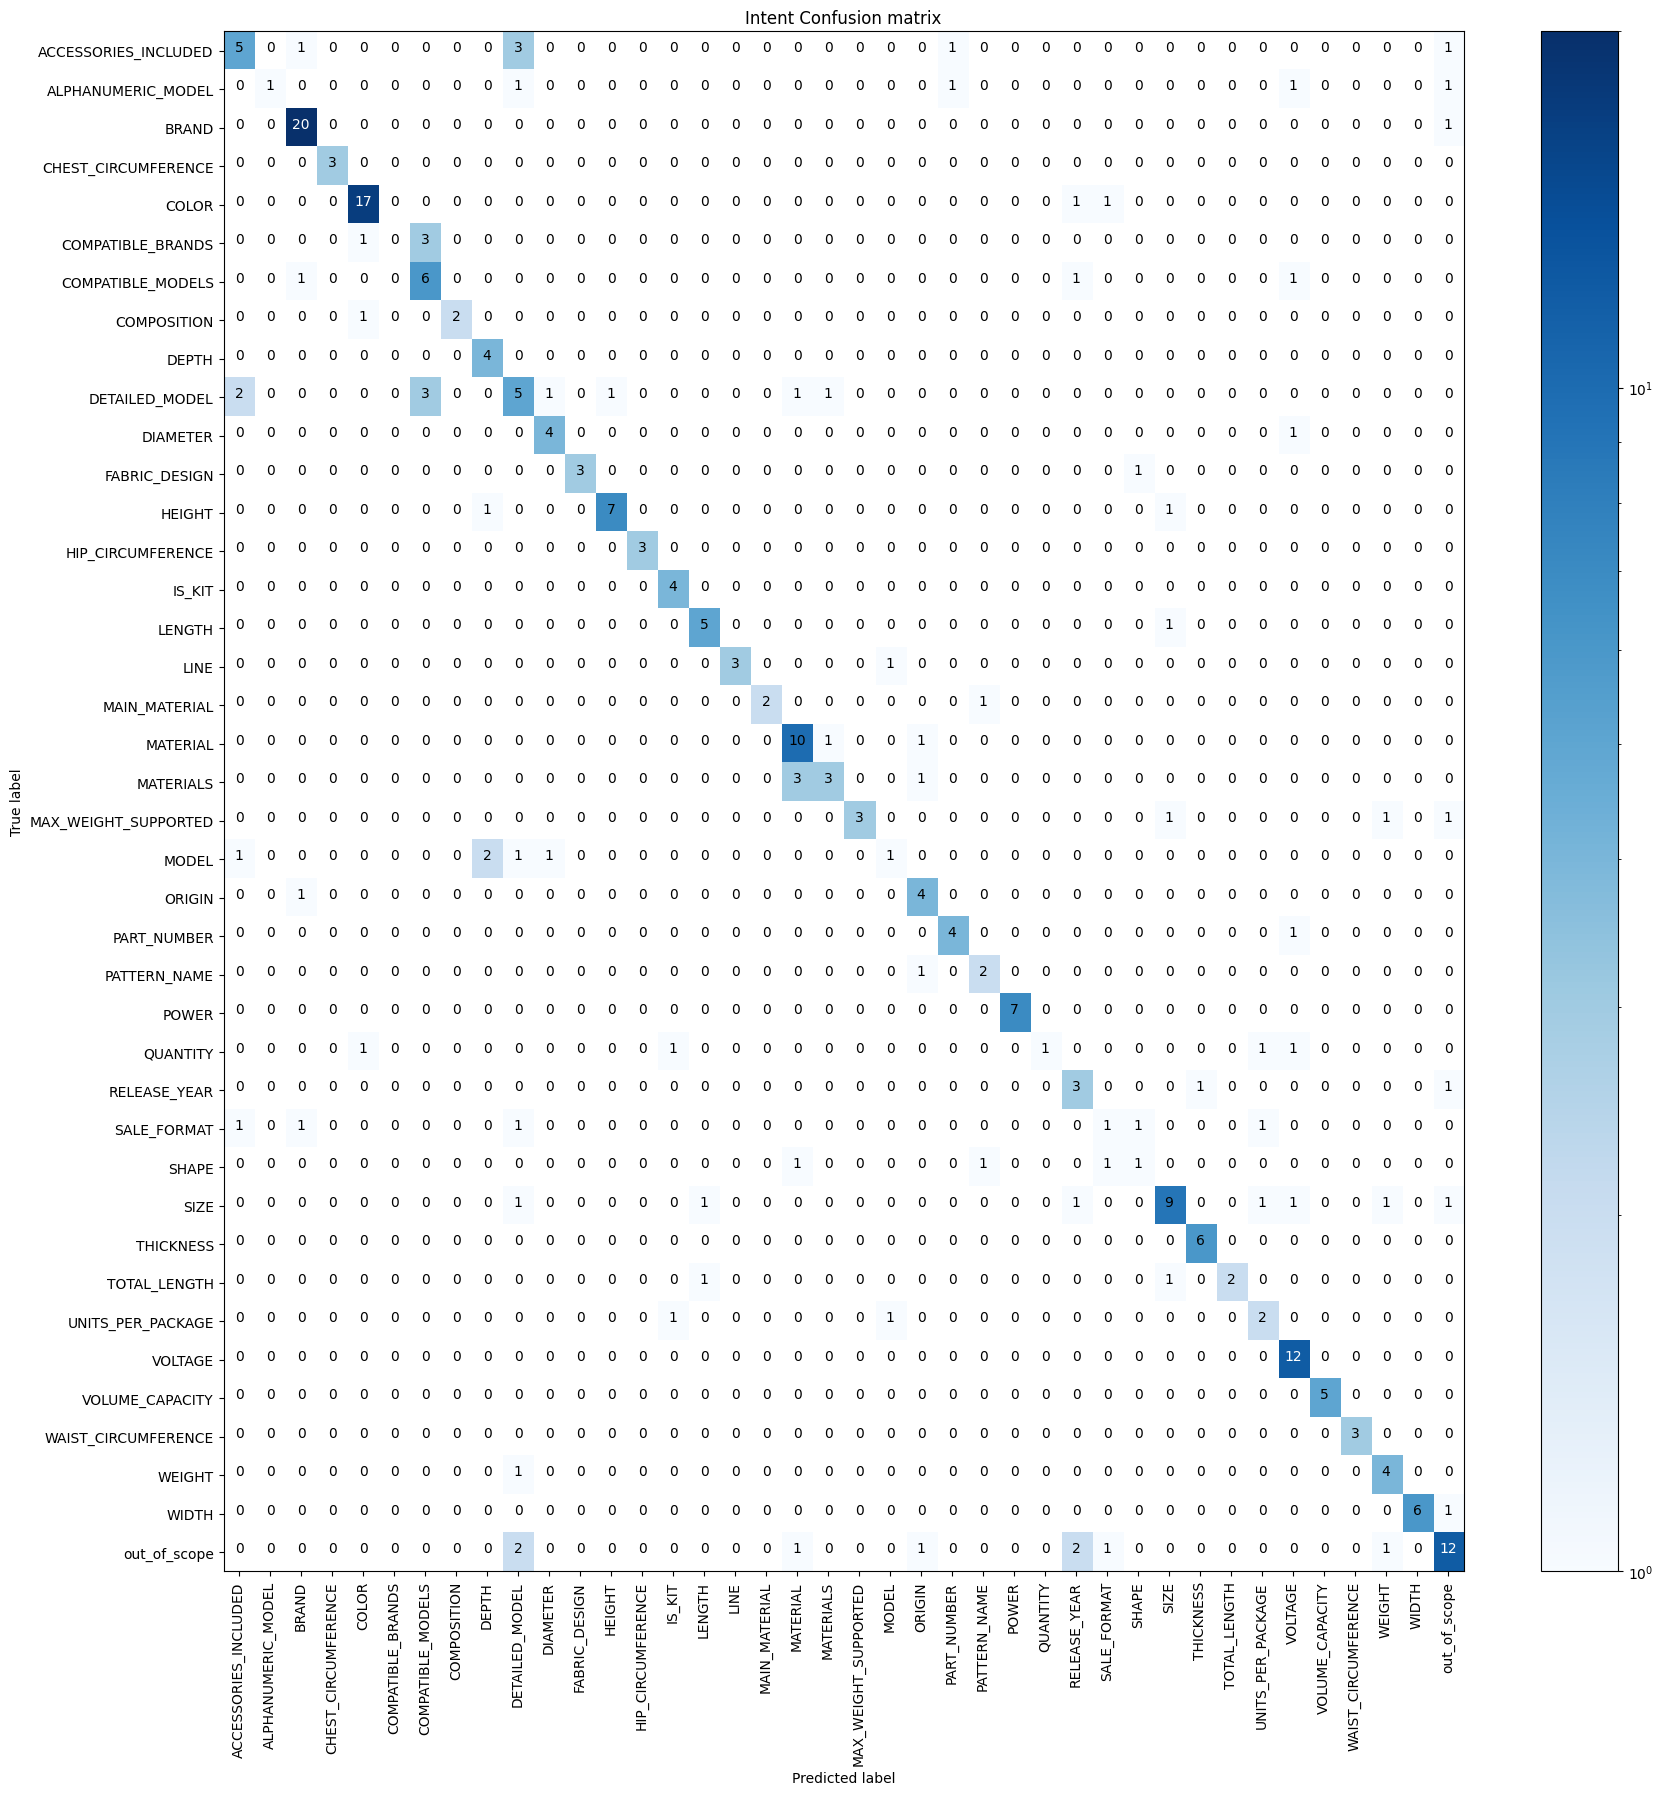
\includegraphics[width=1\linewidth]{figuras/RASA2.png}
	\caption{Matriz de Confusão gerada após teste do modelo RASA2, na configuração com 40 classes.}
	\label{fig:matriz_rasa2}
\end{figure}

\begin{figure}[!ht]
    \centering
	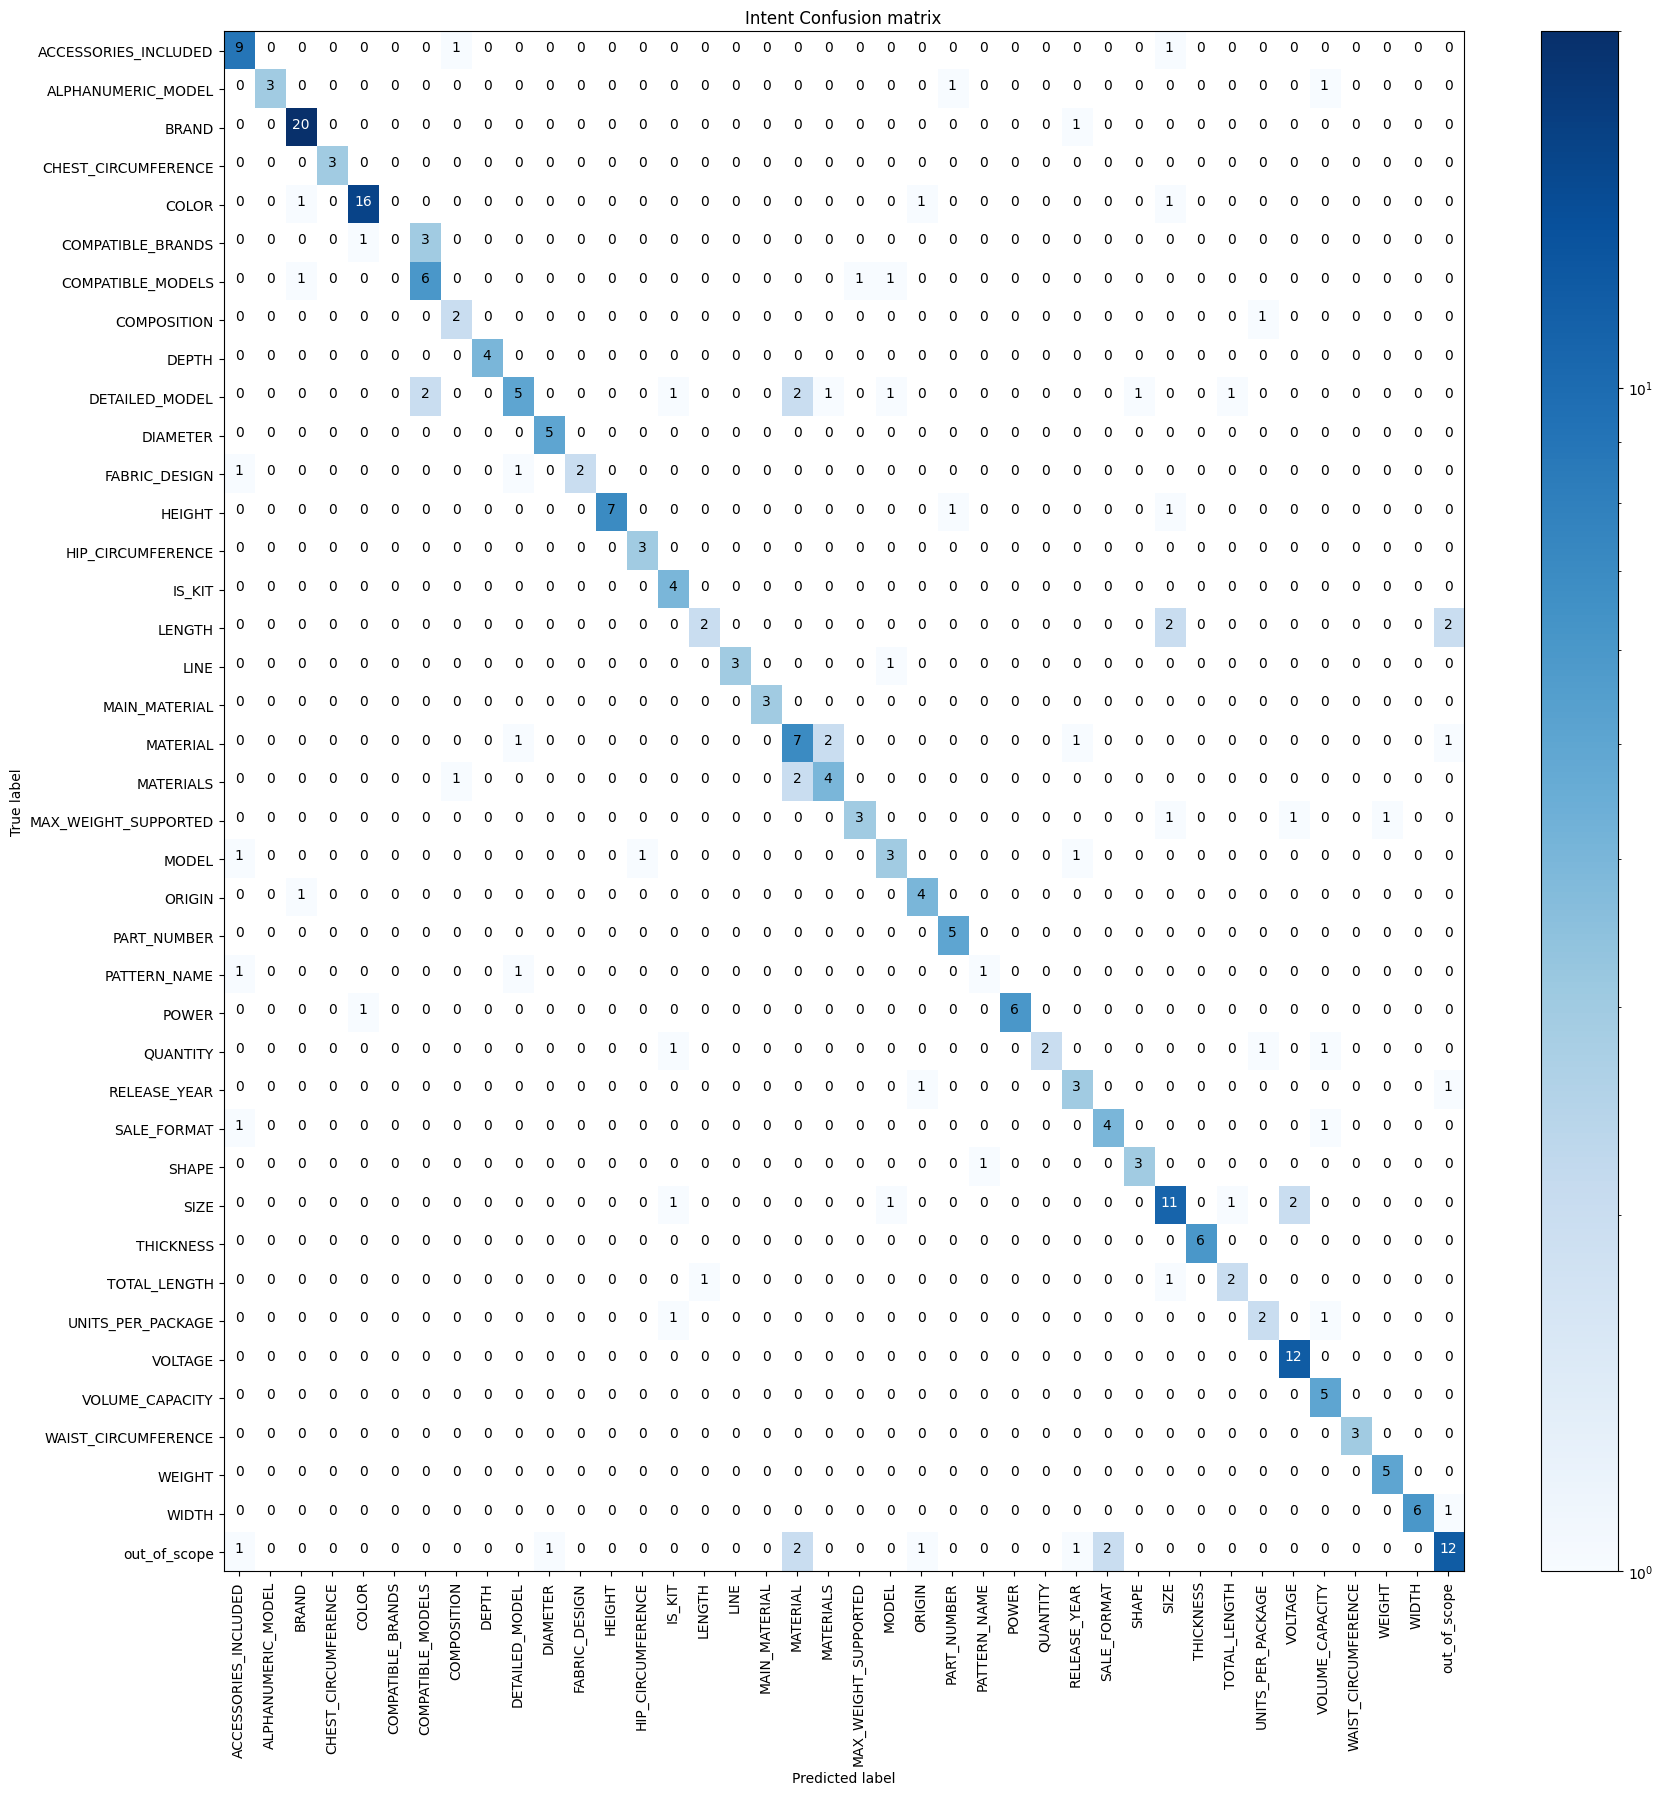
\includegraphics[width=1\linewidth]{figuras/RASA3.png}
	\caption{Matriz de Confusão gerada após teste do modelo RASA3, na configuração com 40 classes.}
	\label{fig:matriz_rasa3}
\end{figure}

\begin{figure}[!ht]
    \centering
	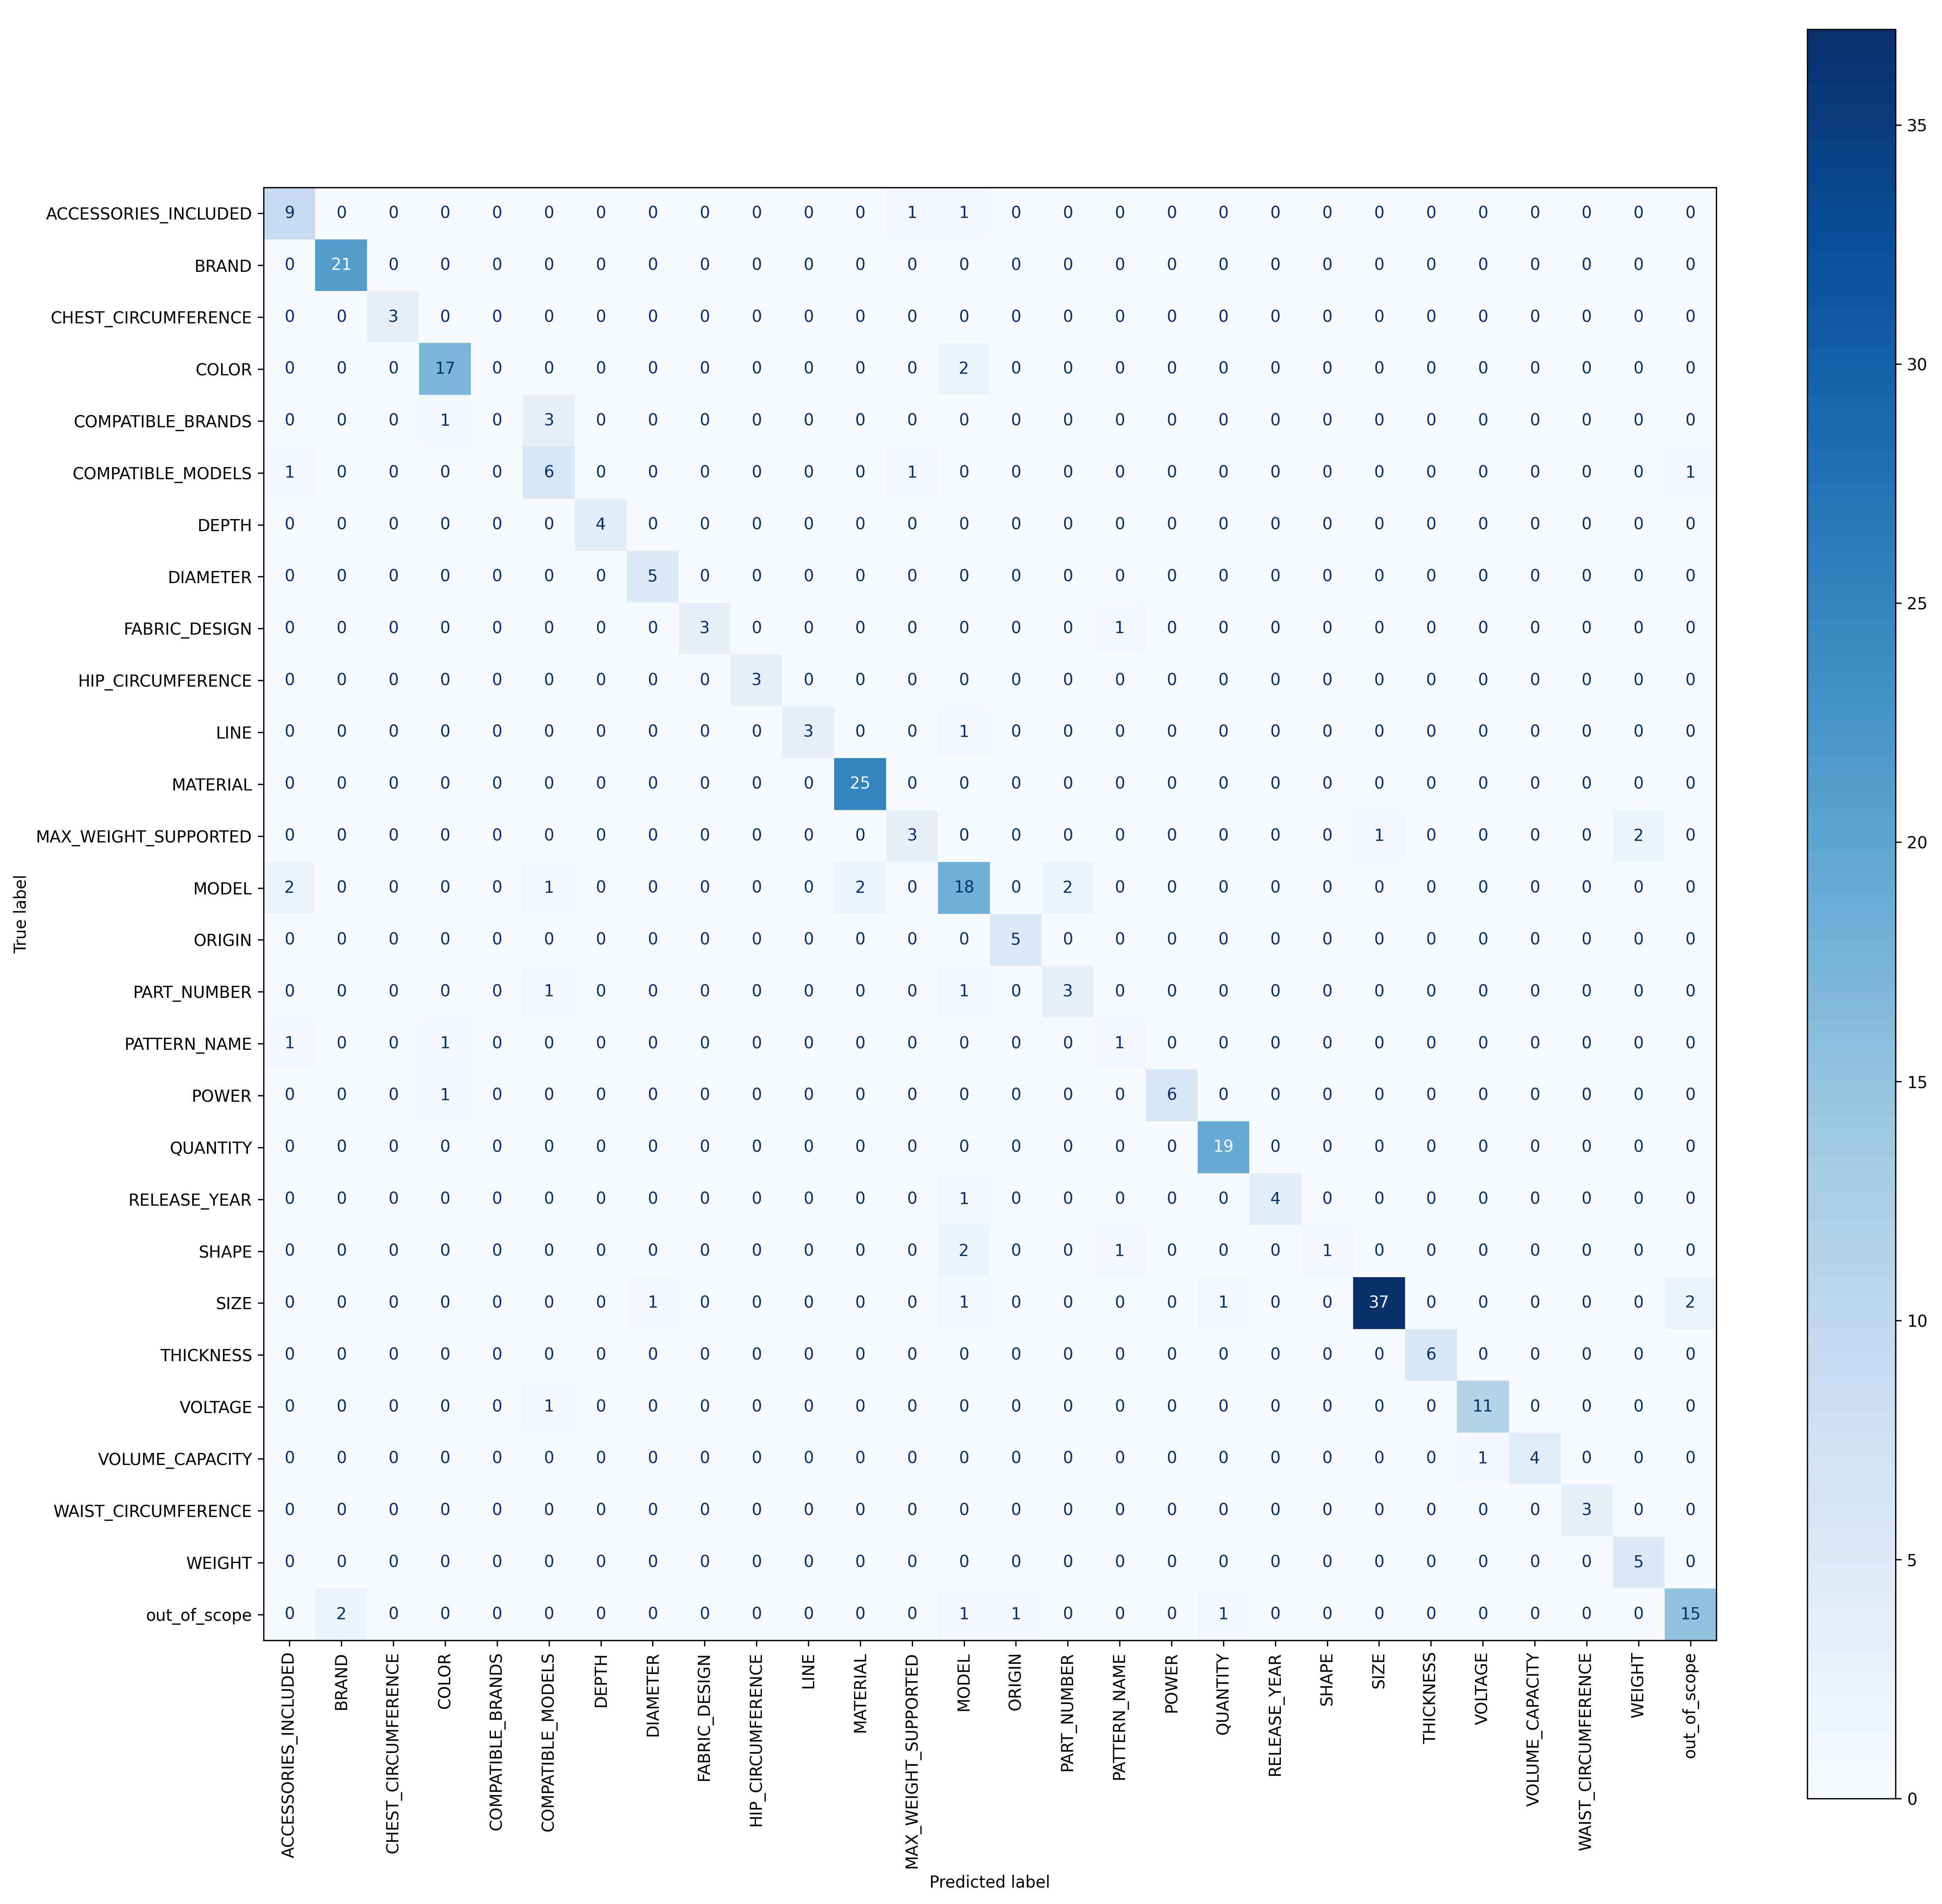
\includegraphics[width=1\linewidth]{figuras/HF2-28_classes.png}
	\caption{Matriz de Confusão gerada após teste do modelo HF2, na configuração com 28 classes.}
	\label{fig:matriz_hf2_28_classes}
\end{figure}

\begin{figure}[!ht]
    \centering
	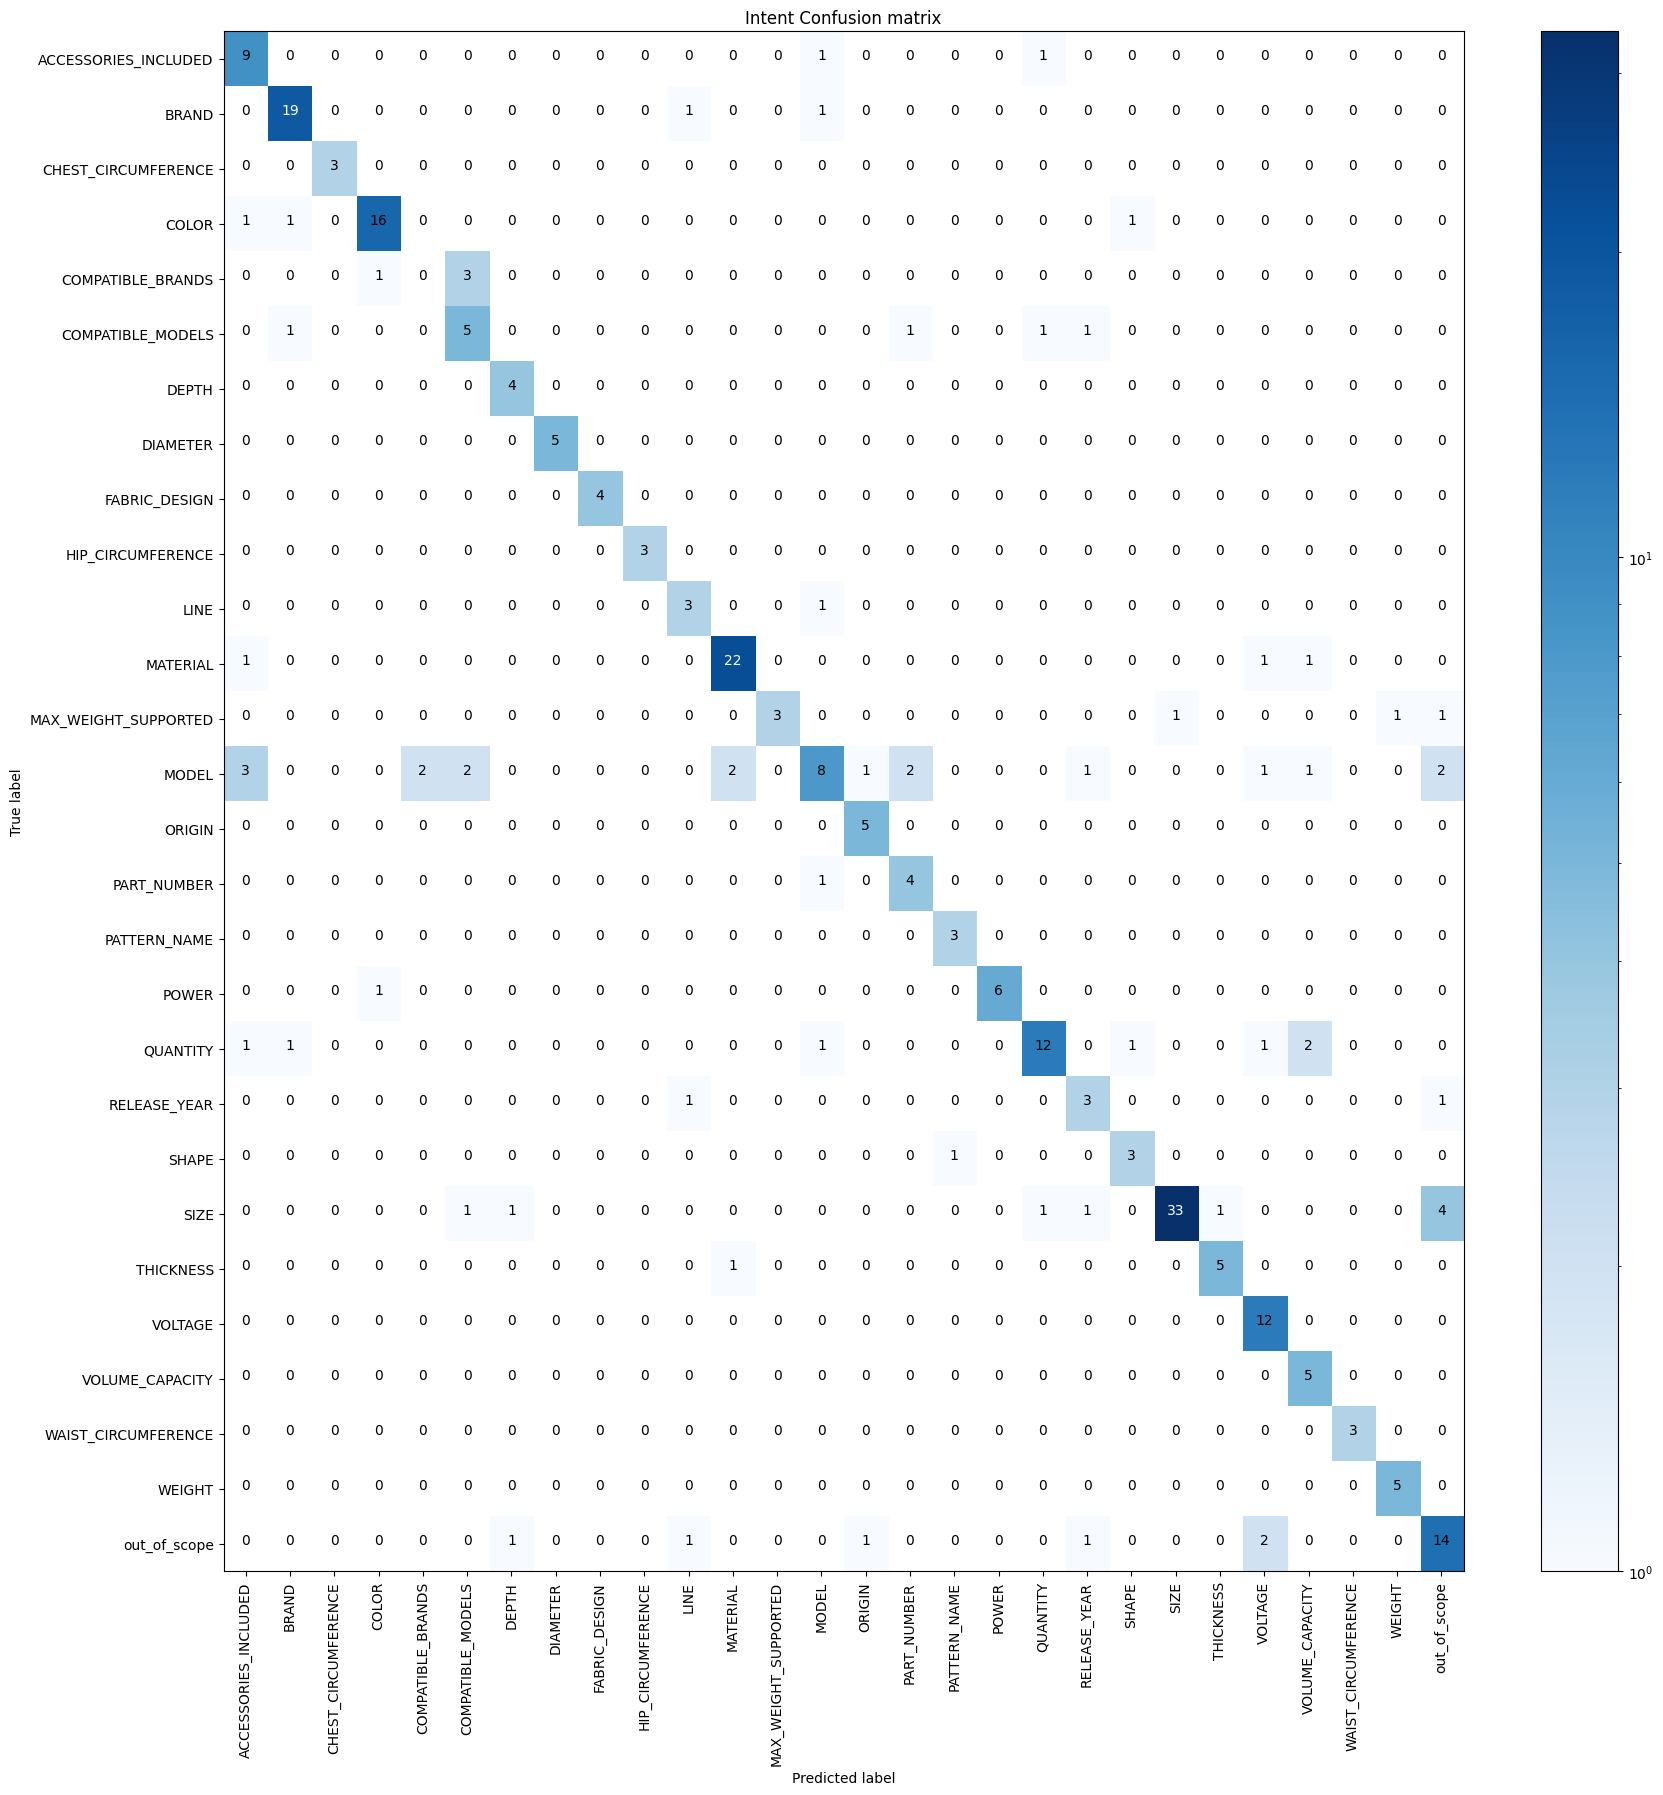
\includegraphics[width=1\linewidth]{figuras/RASA3-28_classes.png}
	\caption{Matriz de Confusão gerada após teste do modelo RASA3, na configuração com 28 classes.}
	\label{fig:matriz_rasa3_28_classes}
\end{figure}
% ----------------------------------------------------------

\end{apendicesenv}


%---------------------------------------------------------------------
% INDICE REMISSIVO
%---------------------------------------------------------------------

\printindex



\end{document}